\documentclass[12pt,a4paper,twoside]{report}

% Load math packages early for XeLaTeX+bidi compatibility
\usepackage{amsmath}
\usepackage{amsfonts}
\usepackage{amssymb}

% ===== PACKAGES =====
\usepackage{iftex}
\ifPDFTeX
  \usepackage[T1]{fontenc}
  \usepackage[utf8]{inputenc}
  \usepackage[french]{babel}
  \usepackage{lmodern}
\else
  \usepackage{fontspec}
\fi
\usepackage{geometry}
\usepackage{fancyhdr}
\usepackage{graphicx}
\usepackage{float}
\usepackage{caption}
\usepackage{subcaption}
\usepackage{listings}
\usepackage{csquotes}
\usepackage[table]{xcolor}
\usepackage{url}
\usepackage{array}
\usepackage{tabularx}
\usepackage{longtable}
\usepackage{multirow}
\usepackage{setspace}
\usepackage{titlesec}
\usepackage{tocloft}
\usepackage{appendix}
\usepackage{enumitem}
\usepackage{hyperref}
\usepackage{pifont}
\usepackage{placeins}

\ifPDFTeX\else
  \usepackage{polyglossia}
  \setmainlanguage{french}
  % \setotherlanguage{arabic}  % Disabled: Amiri font not installed
  \setmainfont{Latin Modern Roman}
  % Arabic font setup disabled - no suitable font available
  % \IfFontExistsTF{Amiri}{
  %   \newfontfamily\arabicfont[Script=Arabic,Scale=1.08]{Amiri}
  % }{
  %   \IfFontExistsTF{Arial}{
  %     \newfontfamily\arabicfont[Script=Arabic,Scale=1.08]{Arial}
  %   }{
  %     \newfontfamily\arabicfont[Script=Arabic,Scale=1.08]{DejaVu Sans}
  %   }
  % }
\fi

\newcommand{\cmark}{\ding{51}}
\newcommand{\warning}{\ding{115}}

% ===== CONFIGURATION DE PAGE =====
\geometry{
  left=3cm,
  right=2.5cm,
  top=2.5cm,
  bottom=2.5cm,
  headheight=16pt
}

% ===== STYLE DES EN-TETES ET PIEDS DE PAGE =====
\pagestyle{fancy}
\fancyhf{}
\fancyhead[LE]{\leftmark}
\fancyhead[RO]{\rightmark}
\fancyfoot[LE,RO]{\thepage}
\renewcommand{\headrulewidth}{0.4pt}
\renewcommand{\footrulewidth}{0pt}

% ===== TITRES =====
\titleformat{\chapter}[hang]{\normalfont\LARGE\bfseries}{\thechapter}{1em}{}
\titlespacing*{\chapter}{0pt}{-30pt}{20pt}
\titleformat{\section}[hang]{\normalfont\Large\bfseries}{\thesection}{1em}{}
\titlespacing*{\section}{0pt}{2ex plus 1ex minus .2ex}{1.5ex plus .2ex}
\titleformat{\subsection}[hang]{\normalfont\large\bfseries}{\thesubsection}{1em}{}
\titlespacing*{\subsection}{0pt}{2.25ex plus 1ex minus .2ex}{1ex plus .2ex}

% ===== ESPACEMENT =====
\onehalfspacing
\setlength{\parindent}{1.5em}
\setlength{\parskip}{0.2em}
\raggedbottom
\setlength{\textfloatsep}{12pt plus 2pt minus 2pt}
\setlength{\floatsep}{10pt plus 2pt minus 2pt}
\setlength{\intextsep}{10pt plus 2pt minus 2pt}
\captionsetup{skip=6pt}

% ===== COULEURS =====
\definecolor{ztblue}{RGB}{35,75,120}
\definecolor{ztgreen}{RGB}{72,130,72}
\definecolor{ztgray}{RGB}{245,247,250}
\definecolor{zlightOrange}{RGB}{250, 191, 143} 

% ===== PAGE TITRE CHAPITRE =====
\newcommand{\chapterpage}[1]{%
  \clearpage
  \thispagestyle{empty}
  \vspace*{\fill}
  \begin{flushleft}
    {\huge\bfseries #1}
  \end{flushleft}
  \vspace*{\fill}
  \clearpage
}

% ===== HYPERLIENS =====
\hypersetup{
  colorlinks=true,
  linkcolor=ztblue,
  urlcolor=ztblue,
  citecolor=ztgreen,
  pdfauthor={Mohammed Sbihi},
  pdftitle={Rapport PFE - Architecture Zero Trust IAM/PIM/PAM},
  pdfsubject={Cybersecurite - Zero Trust},
  pdfkeywords={Zero Trust, IAM, PIM, PAM, Authentik, Tailscale, Wazuh}
}

\begin{document}

% ===== PAGE DE GARDE =====
\begin{titlepage}
  \newgeometry{top=0.9cm, left=0cm, right=0cm, bottom=0cm}
  \thispagestyle{empty}
  \centering

  \IfFileExists{images/USMBA_banner.jpg}{
    
\includegraphics[width=\textwidth]{images/USMBA_banner.jpg}
  }{
    \fcolorbox{black}{ztgray}{\parbox{\textwidth}{\centering\vspace{0.45cm}
        Espace reserve pour le bandeau ENSA/USMBA\vspace{0.45cm}}}
  }

  {\fontsize{23}{26}\selectfont\bfseries Projet de Fin d'Etudes\par}
    \vspace{0.45cm}

  {\large\bfseries Pour l'obtention du dipl\^ome\par}
  \vspace{0.45cm}
  {\fontsize{20}{23}\selectfont\bfseries D'Ing\'enieur d'Etat\par}
  \vspace{0.65cm}
  {\large\bfseries G\'enie des R\'eseaux et T\'el\'ecommunications\par}
  \vspace{0.55cm}
  {\large\bfseries Promotion 2025/2026\par}

  \vspace{0.55cm}
  \noindent\makebox[\textwidth][c]{%
    \colorbox{zlightOrange!30}{%
      \parbox{\dimexpr\textwidth-5cm-2\fboxsep\relax}{%
      \vspace{0.95cm}
      \centering
      {\Large\bfseries Architecture zero trust : réduction de la surface d'attaque par une gestion d'identité et de privilège basé sur le modèle IAM/PIM\par}
      \vspace{0.95cm}
      }%
    }%
  }

  \vspace{0.6cm}
  {\large Stage r\'ealis\'e au sein de : CGI}
  \vspace{0.7cm}

 
    \begin{minipage}[c][2.1cm][c]{4.0cm}
      \centering \includegraphics[width=0.9\textwidth]{images/CGI_logo.png}
    \end{minipage}%
    \vspace{0.7cm}


  \noindent\colorbox{zlightOrange!30}{%
    \parbox{\dimexpr\textwidth-2\fboxsep\relax}{%
      \vspace{1cm}
      \centering
      {\large\bfseries R\'ealis\'e par M. Mohammed Sbihi\par}
      \vspace{0.35cm}
      {\large\bfseries Soutenance le XX/XX/XXXX\par}
      \vspace{0.75cm}
      \begin{minipage}{0.46\textwidth}
        \hspace{0.5cm}
     \hspace{2cm}   \underline{\textbf{Membres de jury :}}\par
        \vspace{0.45cm}
      \hspace{2cm}  \textbf{M.} ENNAJAH YOUSSEF\par
      \hspace{2cm}  \textbf{M.} HRAOUI SAID\par
     \hspace{2cm}   \textbf{M.} ALLA LHOUSSAINE\par
      \end{minipage}%
      \hfill
      \begin{minipage}{0.46\textwidth}
                \vspace{1cm}

        Encadrant Soci\'et\'e\par
        Encadrant ENSAF\par
        Enseignant ENSAF\par
      \end{minipage}
      \vspace{1.75cm}
    }%
  }
\end{titlepage}
\restoregeometry

% ===== PAGES PRELIMINAIRES =====
\pagenumbering{Roman}
\setcounter{page}{1}

\addcontentsline{toc}{chapter}{Dedicace}

\vspace*{1cm}

% Verset coranique
\begin{center}
  \vspace{1cm}
  
\includegraphics[width=0.5\textwidth]{images/in_dedicace.png}
\end{center}

% Texte de dédicace

\begin{center}
  {\Large \textbf{Dédicace}}
\end{center}

\vspace{1.5cm}

\begin{center}
  {\large \textit{C'est avec une grande joie que je dédie ce modeste travail :}}\\[0.5cm]
  À l'être le plus cher de ma vie, ma mère,\\[0.2cm]
  À celui qui a fait de moi un homme, mon père,\\[0.2cm]
  À mes chers frères,\\[0.2cm]
  À tous mes amis de ma promotion \\[0.2cm]
  À tous les membres de ma famille et à toute personne qui occupe une place dans mon cœur,\\[0.5cm]
  Je dédie également ce travail à tous ceux qui ont participé, de près ou de loin, à ma réussite.
\end{center}

\vfill
\clearpage
\chapter*{Remerciements}
\addcontentsline{toc}{chapter}{Remerciements}

\vspace{0.5cm}

Je tiens a exprimer ma profonde gratitude a tous ceux qui ont contribue a la reussite de ce projet de fin d'etudes et a l'elaboration de ce rapport.

\vspace{0.5cm}

\textbf{Avant tout, je remercie Dieu le Tout-Puissant} de m'avoir donne la force, la sante et la volonte necessaires pour mener a bien ce projet. Sa benediction m'a accompagne tout au long de ce parcours.

\vspace{0.5cm}

\textbf{A mon encadrant au sein de CGI Fes,} pour son accueil chaleureux, sa confiance accordee dans le cadre de ce projet Zero Trust, ainsi que ses conseils pratiques et son accompagnement tout au long du stage. Son expertise du terrain et sa vision operationnelle ont ete essentielles pour adapter la solution aux contraintes reelles de l'entreprise.

\vspace{0.5cm}

\textbf{A mon encadrant academique,} pour ses conseils eclaires, son suivi rigoureux et sa disponibilite continue. Ses orientations methodologiques ont ete determinantes dans l'aboutissement de cette realisation.

\vspace{0.5cm}

\textbf{A l'equipe pedagogique} du departement Genie des Telecommunications et Reseaux (GTR), pour la qualite de la formation dispensee, qui m'a permis d'acquerir les competences necessaires a la conception et a l'implementation de cette architecture de cybersecurite.

\vspace{0.5cm}


\textbf{A mes collegues et camarades etudiants,} pour les echanges constructifs, l'entraide et le partage d'idees qui ont contribue a l'avancement de ce travail.

\vspace{0.5cm}

\textbf{A ma famille,} pour son soutien indefectible, sa patience et ses encouragements constants durant les nombreuses heures consacrees a ce projet.

\vspace{0.5cm}
Ce projet n'aurait pu aboutir sans cette convergence de competences, de conseils et d'encouragements. Il temoigne de l'importance de la collaboration dans le domaine de la cybersecurite, ou la mutualisation des connaissances est essentielle pour repondre aux defis securitaires actuels.

\vspace{1cm}

\newpage

\chapter*{Resume}
\addcontentsline{toc}{chapter}{Resume}

Ce projet de fin d'études traite la réduction de la surface d'attaque dans un contexte d'administration de systèmes critiques, à travers une architecture Zero Trust intégrée. Le problème principal identifié est l'existence d'accès privilégiés permanents, peu tracés et insuffisamment corrélés au niveau de criticité des actifs.

La solution proposée combine cinq briques principales : \textbf{Authentik} pour la gestion des identités (IAM), \textbf{Tailscale ACL} pour le contrôle d'accès réseau, une \textbf{application web Flask avec PostgreSQL} pour la gouvernance des demandes, un \textbf{moteur Python Just-in-Time} pour l'approbation/révocation automatisées, et \textbf{Wazuh} pour l'observabilité et la traçabilité de sécurité.

Le flux cible impose qu'aucun accès privilégié ne soit permanent : chaque élévation est demandée, justifiée, approuvée, limitée dans le temps (TTL) puis retirée automatiquement. Les scénarios de validation couvrent l'authentification forte, la demande JIT, l'activation ACL, l'accès SSH pendant la fenêtre autorisée, puis le refus après expiration.

Les résultats attendus montrent une amélioration significative de la posture de sécurité : suppression des accès permanents non justifiés, traçabilité complète du cycle d'accès, et meilleure capacité d'audit et de conformité.
En complément, le chapitre sur la détection d'anomalies présente une solution ciblant les comptes administrateurs. Un pipeline non supervisé, basé sur l'algorithme \textit{Isolation Forest}, analyse des indicateurs temporels et comportementaux (heure, jour, indicateur week-end/nuit, nouveau sous-réseau, nombre d'approbations récentes, type d'action, statut) et entraîne un modèle par administrateur ; tout score élevé (seuil opérationnel typique : 0.60) génère une alerte enrichie envoyée au SIEM pour investigation. Les visualisations facilitent l'interprétation des résultats et la traçabilité des détections.

\textbf{Mots-cles :} Zero Trust, IAM, PIM, PAM, Authentik, Tailscale, JIT, ACL, Wazuh, cybersecurite.

\clearpage

\chapter*{Abstract}
\addcontentsline{toc}{chapter}{Abstract}

This final-year project addresses attack-surface reduction in a privileged-access context through an integrated Zero Trust architecture. The main issue identified in the initial environment is the presence of persistent privileged access, limited traceability, and weak correlation between access rights and asset criticality.

The proposed solution combines five main building blocks: \textbf{Authentik} for Identity and Access Management (IAM), \textbf{Tailscale ACL} for network-level authorization, a \textbf{Flask web application with PostgreSQL} for request lifecycle governance, a \textbf{Python Just-in-Time engine} for automated approval and revocation, and \textbf{Wazuh} for centralized monitoring and auditability.

The target workflow enforces a strict principle: no permanent privileged access. Every elevation request must be justified, approved, time-bounded (TTL), and automatically revoked. Validation scenarios cover strong authentication, JIT request creation, ACL activation, SSH access during authorized time windows, and automatic denial after expiration.

Expected outcomes include a stronger security posture, full end-to-end traceability of privileged access, and improved compliance evidence for audit processes.

\textbf{Keywords:} Zero Trust, IAM, PIM, PAM, Authentik, Tailscale, JIT, ACL, Wazuh, cybersecurity.

\clearpage

% \chapter*{\textarabic{ملخص}}
\addcontentsline{toc}{chapter}{ملخص}

\begin{Arabic}

يتناول مشروع نهاية الدراسة هذا تقليص مساحة الهجوم في سياق إدارة الأنظمة الحساسة، وذلك من خلال بنية تحتية متكاملة قائمة على مبدأ "انعدام الثقة" (Zero Trust). تكمن الإشكالية الرئيسية التي تم تحديدها في وجود صلاحيات وصول امتيازية دائمة، تفتقر إلى التتبع الدقيق ولا ترتبط بشكل كافٍ بمستوى حساسية الأصول الرقمية.

تعتمد الحلول المقترحة على دمج خمس ركائز أساسية: Authentik لإدارة الهويات (IAM)، و Tailscale ACL للتحكم في الوصول إلى الشبكة، وتطبيق ويب Flask مع قاعدة بيانات PostgreSQL لحوكمة الطلبات، ومحرك Python (Just-in-Time) للأتمتة والموافقة أو الإلغاء التلقائي، بالإضافة إلى Wazuh لضمان قابلية المراقبة والتتبع الأمني.

يفرض مسار العمل المستهدف عدم وجود أي وصول امتيازي دائم؛ حيث يتم طلب كل رفع للصلاحيات وتبريره والموافقة عليه، مع تقييده بفترة زمنية محددة (TTL) ثم سحبه تلقائيًا. تشمل سيناريوهات التحقق: المصادقة القوية، طلب الوصول الآني (JIT)، تفعيل الـ ACL، والوصول عبر بروتوكول SSH خلال النافذة الزمنية المسموح بها، متبوعًا برفض الوصول فور انتهاء الصلاحية.

تُظهر النتائج المتوقعة تحسنًا ملحوظًا في الوضع الأمني من خلال: إلغاء الوصول الدائم غير المبرر، التتبع الكامل لدورة حياة الوصول، وتعزيز القدرة على التدقيق والامتثال للمعايير الأمنية.

\textbf{الكلمات المفتاحية:} Zero Trust، IAM، PIM، PAM، Authentik، Tailscale، JIT، ACL، Wazuh، الأمن السيبراني.

\end{Arabic}

\clearpage  % Disabled: Arabic language support disabled
\chapter*{Liste des abreviations}
\addcontentsline{toc}{chapter}{Liste des abreviations}

\begin{longtable}{>{\bfseries}p{0.18\textwidth} p{0.75\textwidth}}
ACL & Access Control List \\
API & Application Programming Interface \\
CVE & Common Vulnerabilities and Exposures \\
CVSS & Common Vulnerability Scoring System \\
IAM & Identity and Access Management \\
JIT & Just-in-Time \\
MFA & Multi-Factor Authentication \\
OIDC & OpenID Connect \\
PAM & Privileged Access Management \\
PFE & Projet de Fin d'Etudes \\
PIM & Privileged Identity Management \\
RBAC & Role-Based Access Control \\
SIEM & Security Information and Event Management \\
SOC & Security Operations Center \\
SSO & Single Sign-On \\
TTL & Time To Live \\
\end{longtable}

\clearpage

\chapter*{Introduction generale}
\addcontentsline{toc}{chapter}{Introduction generale}

Le contexte de ce projet est marque par la multiplication des cyberattaques visant les acces privilegies, alors que les modeles perimetriques traditionnels ne suffisent plus a proteger des environnements hybrides et distribues. Dans ce cadre, le principe Zero Trust, formalise notamment par le NIST SP 800-207, impose de ne jamais faire confiance par defaut et de verifier chaque demande d'acces.

La problematique adressee dans ce rapport est la suivante: comment supprimer les acces permanents tout en preservant la capacite operationnelle des equipes techniques? La reponse proposee repose sur une gouvernance JIT fondee sur l'authentification forte, l'approbation explicite, la limitation temporelle des privileges et la tracabilite systematique des actions.

La solution integre Authentik pour l'IAM, une application Flask pour la gouvernance des demandes, Tailscale ACL pour l'application des droits reseau, un moteur Python pour l'activation et la revocation temporaires, et Wazuh pour l'observabilite et l'audit.

Le rapport est structure en six chapitres. Le premier presente le contexte et les risques lies aux acces privilegies. Le deuxieme positionne la solution par rapport aux approches existantes. Le troisieme detaille la conception de l'architecture Zero Trust. Le quatrieme decrit l'implementation. Le cinquieme presente la validation et les tests. Le sixieme discute les limites et les travaux futurs, avant la conclusion generale et les annexes.

\clearpage

\clearpage
\setcounter{tocdepth}{1}
\setcounter{secnumdepth}{3}
\tableofcontents
\clearpage

\listoffigures
\clearpage

\listoftables
\clearpage

% ===== CORPS DU RAPPORT =====
\pagenumbering{arabic}
\setcounter{page}{1}

\chapterpage{Chapitre 1 : Contexte et analyse des risques}
\chapter{Contexte et analyse des risques}

\section{Introduction du chapitre}
Ce chapitre présente d'abord l'organisme d'accueil et le périmètre technique du projet, puis il formalise les risques liés aux accès privilégiés et l'objectif de sécurisation qui a guidé la conception.

\chapter{Representation CGI}

\section{Introduction du chapitre}
Ce chapitre introduit la representation CGI du projet (Contexte, Gouvernance, Implementation). Il sera complete avec le contenu detaille fourni ulterieurement.

\section{Objectif de la representation}
La representation CGI sert a presenter, en ouverture du document, une vue synthetique de la demarche:
\begin{itemize}
    \item \textbf{Contexte}: problemes de securite adresses et contraintes d'exploitation;
    \item \textbf{Gouvernance}: regles de decision, responsabilites et cycle d'approbation;
    \item \textbf{Implementation}: traduction technique dans l'architecture Zero Trust deployee.
\end{itemize}

\section{Elements a detailler (a completer)}
Le contenu final de cette section sera ajoute apres reception des elements attendus:
\begin{enumerate}
    \item definition operationnelle de la composante \textbf{C};
    \item definition operationnelle de la composante \textbf{G};
    \item definition operationnelle de la composante \textbf{I};
    \item articulation CGI avec les chapitres suivants du rapport.
\end{enumerate}

\section{Conclusion du chapitre}
La representation CGI pose le cadre de lecture du rapport et prepare l'analyse detaillee presentee dans les chapitres suivants.


\section{Perimetre critique}
Le périmètre critique concerne les serveurs d'administration, les machines cibles SSH, les composants réseau et les services de supervision utilisés pour les interventions de remédiation. Ces ressources concentrent les droits les plus sensibles et justifient un contrôle strict des élévations de privilège.

\section{Analyse des risques lies aux acces privilegies}
Trois scénarios principaux ont été retenus :
\begin{itemize}
  \item un compte permanent volé ou réutilisé abusivement ;
  \item une session privilégiée non tracée ou mal reliée à son initiateur ;
  \item une accumulation progressive de droits non révoqués.
\end{itemize}

\begin{figure}[H]
  \centering
  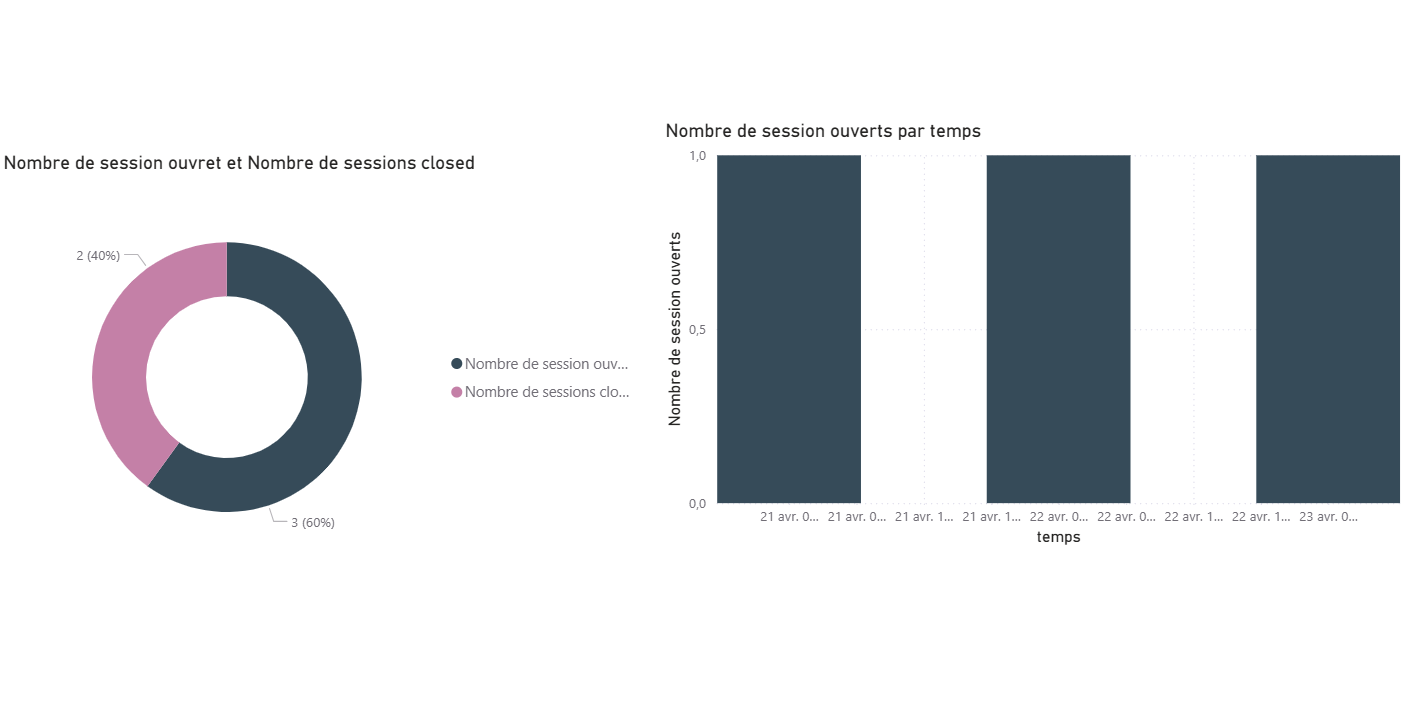
\includegraphics[width=0.95\textwidth]{images/Authentification IAM nombre de session ouvert et fermer dasn un anneau et dans des bar la bar est le nombre de session ouvert par temps.png}
  \caption{Synthèse Power BI des sessions IAM ouvertes et fermées dans le temps.}
  \label{fig:powerbi-sessions-iam}
\end{figure}

Cette vue met en évidence les volumes de sessions et leur évolution temporelle. Elle aide à justifier le passage vers une gouvernance Zero Trust avec limitation de durée et traçabilité explicite.

\section{Objectifs SMART du projet}
Les objectifs retenus sont les suivants :
\begin{itemize}
  \item supprimer les accès permanents non justifiés ;
  \item tracer 100\% des élévations de privilège ;
  \item imposer un TTL maximal configurable selon le type d'accès.
\end{itemize}

\section{Conclusion du chapitre}
L'analyse montre que la réduction de la surface d'attaque passe d'abord par la maîtrise des accès privilégiés, leur temporalité et leur journalisation. Ce constat motive directement le choix d'une architecture Zero Trust.
\chapterpage{Chapitre 2 : Etat de l'art et positionnement}
\chapter{État de l'art et positionnement}

\section{Introduction du chapitre}

Ce chapitre constitue le fondement conceptuel du projet en positionnant la solution proposée dans le contexte de la sécurité informatique contemporaine et des approches Zero Trust. Nous articulerons notre travail autour de trois axes principaux :

\begin{enumerate}
    \item \textbf{Les principes du modèle Zero Trust} : son émergence, ses fondements théoriques et son cadre de référence selon le NIST SP 800-207
    \item \textbf{Les briques technologiques associées}: IAM (Identity and Access Management), PIM (Privileged Identity Management) et PAM (Privileged Access Management), avec leurs rôles respectifs et complémentarités
    \item \textbf{L'analyse de l'écosystème existant} : solutions commerciales et open source, leurs avantages, limitations et positionnement par rapport à nos objectifs
\end{enumerate}

Cette analyse critique nous permettra de justifier les choix architecturaux et technologiques retenus pour la mise en œuvre d'une infrastructure Zero Trust au sein de CGI, adaptée aux contraintes d'une organisation moyenne.

\section{Zero Trust : principes, fondements et architecture de référence}

\subsection{Contexte et évolution du modèle de sécurité}

La sécurité informatique a longtemps reposé sur un modèle de périmètre : une distinction nette entre un intérieur de confiance (l'entreprise) et un extérieur non fiable (Internet). Ce modèle de château-et-douves, popularisé dans les années 1990 et 2000, supposait que les menaces proviendraient essentiellement de l'extérieur. Cependant, cette approche présente plusieurs faiblesses majeures :

\begin{itemize}
    \item \textbf{Explosion du périmètre} : avec le cloud computing, le télétravail et la mobilité, le périmètre réseau s'est fragmenté et étendu de façon ingérable.
    \item \textbf{Menaces internes}: Les données compromises montrent que 30-40\% des incidents impliquent des accès abusifs internes ou des comptes compromis.
    \item \textbf{Confiance implicite dangereuse}: L'accès unique au réseau interne accordait trop de privilèges par défaut, multipliant les surfaces d'attaque.
    \item \textbf{Convergence des menaces} : les attaquants ne respectent plus les frontières réseau ; ils opèrent via des vecteurs hybrides (cloud, SaaS, API, etc.).
\end{itemize}

Face à ces enjeux, le concept de \textit{Zero Trust} a émergé en 2010 avec le modèle BeyondCorp de Google, proposant une alternative fondamentale : \textbf{ne faire confiance à aucune entité par défaut}, qu'elle soit utilisateur, appareil, application ou réseau. Chaque accès doit être vérifié, authentifié et autorisé dans un contexte continu.

\subsection{Principes fondamentaux du Zero Trust}

Le cadre de référence établi par le NIST SP 800-207 (2020) et amélioré par les directives NIST CSF 2.0 (2024) définit les principes suivants du Zero Trust :

\begin{enumerate}
    \item \textbf{Vérification continue de l'identité} : chaque utilisateur, appareil et application doit être authentifié et autorisé à chaque tentative d'accès, indépendamment de la localisation ou du réseau.
    
    \item \textbf{Moindre privilège (Principle of Least Privilege - PoLP)}: Un utilisateur, un appareil ou une application ne reçoit que les permissions minimales nécessaires pour accomplir sa tâche, durant la plus courte période possible.
    
    \item \textbf{Absence de confiance implicite}: Aucune entité (utilisateur, machine, service) n'est intrinsèquement fiable. La confiance doit être établie par vérification et validation.
    
    \item \textbf{Évaluation dynamique du contexte}: Les décisions d'accès doivent considérer des facteurs dynamiques: localisation géographique, statut de l'appareil (patches, antivirus), heure, sensibilité de la ressource, etc.
    
    \item \textbf{Sécurité par défaut (Secure by Default)}: Les configurations doivent refuser l'accès par défaut et l'accorder explicitement après validation.
    
    \item \textbf{Journalisation et auditabilité complètes} : chaque action, chaque tentative d'accès, chaque décision de contrôle doit être enregistrée et exploitable pour la forensie et l'amélioration continue.
\end{enumerate}

\subsection{Architecture de référence Zero Trust}

Le NIST SP 800-207 propose une architecture composée de plusieurs domaines logiques interconnectés:

\begin{itemize}
    \item \textbf{Domaine d'accès (Access Domain)}: L'utilisateur ou l'entité qui demande l'accès
    \item \textbf{Domaine de ressources (Resource Domain)}: La ressource, service ou donnée protégée
    \item \textbf{Domaine administratif (Administrative Domain)}: Les systèmes de gestion d'identité, de politique et de contrôle
    \item \textbf{Point de décision et d'exécution (Policy Decision Point - PDP et Policy Enforcement Point - PEP)}: Respectivement responsables de l'évaluation des politiques et de leur application
    \item \textbf{Collecteur d'événements (Event Collector)}: Centralisé pour la journalisation et l'analyse
\end{itemize}

La mise en œuvre d'une architecture Zero Trust ne consiste pas simplement à ajouter de la technologie, mais à repenser la relation entre l'utilisateur, les ressources et les contrôles de sécurité.

\section{Gestion des identités et des accès: IAM, PIM, PAM}

\subsection{IAM (Identity and Access Management)}

L'IAM est la couche fondamentale qui répond à trois questions critiques:

\begin{enumerate}
    \item \textbf{Qui es-tu?} (Authentification): Vérification de l'identité par des facteurs (mot de passe, MFA, certificats, etc.)
    \item \textbf{Que peux-tu faire?} (Autorisation): Attribution des permissions basée sur des politiques et des rôles (RBAC, ABAC)
    \item \textbf{D'où viens-tu?} (Fédération): Reconnaissance d'identités provenant d'autres systèmes (SSO, OIDC, SAML)
\end{enumerate}

Les fonctions principales de l'IAM incluent:
\begin{itemize}
    \item Gestion du cycle de vie des utilisateurs (onboarding, changements de rôle, départ)
    \item Attribution et révocation des permissions
    \item Authentification multi-facteur (MFA/2FA)
    \item Single Sign-On (SSO) et fédération d'identités
    \item Gestion des entités de service (service accounts)
    \item Reporting et auditabilité des accès
\end{itemize}

\subsection{PIM (Privileged Identity Management)}

Le PIM traite spécifiquement les identités et les accès privilégiés. Contrairement à l'IAM classique qui gère les accès standards, le PIM adresse une problématique critique: \textbf{la gestion des comptes avec privilèges d'administrateur ou d'accès système}.

Les menaces liées aux identités privilégiées sont disproportionnées:
\begin{itemize}
    \item 45-60\% des violations impliquent un compte administrateur compromis (Verizon DBIR 2024)
    \item Un compte administrateur peut donner accès à l'ensemble du système sans restriction
    \item Les comptes partagés (legacy) multiplient le risque et réduisent la responsabilité
\end{itemize}

Le PIM répond par:
\begin{itemize}
    \item \textbf{Just-In-Time (JIT) Access}: Octroi temporaire et à la demande de privilèges, révoqué automatiquement après une durée définie (TTL - Time To Live)
    \item \textbf{Workflow d'approbation}: Demandes de privilèges soumises à validation hiérarchique ou basée sur des conditions
    \item \textbf{Session Recording}: Enregistrement de toutes les actions d'administrateur pour auditabilité complète
    \item \textbf{Check-Out/Check-In}: Mécanisme de restitution des credentials après l'accès
    \item \textbf{Isolation de domaine}: Séparation logique entre accès standard et accès privilégié
\end{itemize}

\subsection{PAM (Privileged Access Management)}

Le PAM est une couche complémentaire au PIM, focalisée sur l'application et l'enforcement des politiques d'accès privilégié. Tandis que le PIM gère \textit{qui} accède et \textit{quand}, le PAM gère \textbf{comment} et \textbf{sur quoi} ils accèdent.

Les responsabilités du PAM incluent:
\begin{itemize}
    \item \textbf{Credential Vaulting}: Stockage sécurisé des credentials (comptes root, clés API, certificates)
    \item \textbf{Proxying sécurisé}: Interception et relais des connexions privilégiées à travers un point de contrôle centralisé
    \item \textbf{Policy Enforcement Point}: Application des politiques réseau et des ACL au moment de l'accès
    \item \textbf{Alertes en temps réel}: Détection des comportements anormaux ou déviations de politiques
    \item \textbf{Intégration SIEM}: Flux d'événements vers les systèmes de détection d'intrusion
\end{itemize}

\subsection{Complémentarité IAM-PIM-PAM et intégration}

Ces trois composantes ne sont \textit{pas} redondantes mais complémentaires dans une stratégie Zero Trust:

\begin{itemize}
    \item \textbf{IAM} répond: "Autorise-t-on cet utilisateur à demander l'accès?"
    \item \textbf{PIM} répond: "Approuvons-nous cette demande? Accordons-nous ces privilèges temporairement?"
    \item \textbf{PAM} répond: "Appliquons-nous strictement les politiques d'accès? Enregistrons-nous et alertons-nous?"
\end{itemize}

L'intégration verticale IAM → PIM → PAM garantit une chaîne de traçabilité complète et une défense en profondeur.

\section{Solutions existantes: analyse du marché}

\subsection{Solutions commerciales}

\subsubsection{CyberArk}

CyberArk est le leader incontesté du marché PAM/PIM avec une couverture très large:
\begin{itemize}
    \item Gestion complète des credential vaults (secrets, clés API, certificates)
    \item Session recording et playback haute qualité
    \item Intégration native avec Active Directory, Cloud (AWS, Azure, GCP)
    \item SIEM et endpoint detection intégrés
    \item Prix: 50 000-500 000 EUR/an selon la taille
    \item Limitations: Coûteux, complexité d'implémentation, ecosystème propriétaire
\end{itemize}

\subsubsection{BeyondTrust}

BeyondTrust offre une suite complète et modulaire:
\begin{itemize}
    \item Remote Support (accès technicient sécurisé)
    \item Privileged Access Management (PAM)
    \item Identity Governance (IAM)
    \item Cloud-native et on-premises
    \item Prix: 30 000-300 000 EUR/an
    \item Avantages: Modularité, interface intuitive, cloud-ready
    \item Limitations: Moins d'intégrations SIEM que CyberArk
\end{itemize}

\subsubsection{Delinea (Thycotic)}

Delinea propose une approche plus légère et moderne:
\begin{itemize}
    \item Secret Server: Vault centralisé pour credentials et secrets
    \item Privileged Session Manager: Proxying et recording
    \item Cloud-ready et scalable
    \item Prix: 15 000-150 000 EUR/an
    \item Avantages: Meilleur rapport performance/coût
    \item Limitations: Moins mature que CyberArk en termes de détection d'anomalies
\end{itemize}

\subsection{Solutions open source et hybrides}

\subsubsection{Authentik (OIDC/SAML Provider)}

Authentik est une solution IAM open source moderne:
\begin{itemize}
    \item Autohébergée ou cloud-managed
    \item Support OIDC, SAML, OAuth2
    \item Gestion des workflows d'approbation
    \item MFA et risk-based authentication
    \item Intégration LDAP/Active Directory
    \item Coût: Gratuit (open source) ou 200-5 000 EUR/an (managed)
    \item Avantages: Légère, flexible, pas de licence au nombre d'utilisateurs
    \item Limitations: Pas de credential vaulting natif, PAM limité
\end{itemize}

\subsubsection{Tailscale (Network Access Control)}

Tailscale propose une VPN moderne basée sur WireGuard et le zero trust:
\begin{itemize}
    \item Mesh VPN avec chiffrement end-to-end
    \item ACL granulaires (par utilisateur, groupe, tag)
    \item Appliance et point de sortie flexibles
    \item Intégration Okta, Azure AD
    \item Prix: Gratuit (personnel) ou 50-1 000 EUR/utilisateur/an
    \item Avantages: Déploiement rapide, UX simple, multi-plateforme
    \item Limitations: Accent sur accès réseau, pas de credential management
\end{itemize}

\subsubsection{Teleport (SSH/RDP/Kubernetes Access)}

Teleport est un gestionnaire d'accès pour environnements cloud-native:
\begin{itemize}
    \item Accès SSH/RDP/Kubernetes centralisé
    \item Session recording complet
    \item RBAC et audit trails
    \item CoS gratuit (open source) ou payante (enterprise)
    \item Avantages: Excellent pour DevOps/Cloud, API-first
    \item Limitations: Orienté infrastructure, pas de IAM complet
\end{itemize}

\subsubsection{Border0 (Zero Trust Network)}

Border0 propose un service d'accès zero trust léger:
\begin{itemize}
    \item Connexions sécurisées aux resources sans VPN
    \item Logging et audit centralisés
    \item Intégration OAuth/OIDC
    \item Prix: Freemium ou 100-500 EUR/mois
    \item Avantages: Très simple à déployer, approche moderne
    \item Limitations: Moins mature, fonctionnalités limitées
\end{itemize}

\section{Analyse comparative et justification des choix retenus}

\subsection{Critères d'évaluation}

Nous avons défini une matrice d'évaluation basée sur les critères suivants:

\begin{table}[h]
\centering
\begin{tabularx}{\textwidth}{|l|X|X|X|X|}
\hline
\textbf{Critère} & \textbf{Pondération} & \textbf{Justification} & \textbf{Contexte} \\
\hline
Couverture IAM & 25\% & Authentification multi-facteur, SSO, fédération LDAP/AD essentielles & Gestion 100+ utilisateurs \\
\hline
Gestion des privilèges & 25\% & JIT, approbation, session recording pour conformité & Infrastructure sensible \\
\hline
Facilité de déploiement & 15\% & Délai de mise en place limité, ressources internes réduites & Contexte PME/PMI \\
\hline
Coût TCO (5 ans) & 15\% & Budget limité, pas de budget illimité pour technologie & CGI groupe, mais direction locale autonome \\
\hline
Flexibilité et extensibilité & 10\% & Capacité à adapter, intégrer, modifier selon besoins métier & Évolution future des besoins \\
\hline
Auditabilité et conformité & 10\% & Logs complets, traçabilité, RGPD et réglementations applicables & Secteur finance/santé potentiel \\
\hline
\end{tabularx}
\caption{Matrice d'évaluation des solutions Zero Trust}
\end{table}

Cette table définit les six critères clés utilisés pour comparer les solutions. La pondération reflète l'importance relative de chaque critère dans le contexte CGI: la couverture IAM et la gestion des privilèges sont les plus critiques (25\% chacune), tandis que la flexibilité, l'auditabilité et la conformité jouent un rôle complémentaire. Cette approche garantit un choix équilibré entre fonctionnalité, coût et opérationnel.
\newpage
\subsection{Scores comparatifs}

\begin{table}[h]
\centering
\begin{tabularx}{\textwidth}{|l|c|c|c|c|c|c|c|}
\hline
\textbf{Solution} & \textbf{IAM} & \textbf{Priv.} & \textbf{Deploy} & \textbf{Coût} & \textbf{Flex.} & \textbf{Audit} & \textbf{Score} \\
\hline
CyberArk & 9/10 & 10/10 & 5/10 & 3/10 & 6/10 & 10/10 & \textbf{7.5/10} \\
\hline
BeyondTrust & 8/10 & 9/10 & 6/10 & 5/10 & 7/10 & 9/10 & \textbf{7.6/10} \\
\hline
Authentik + Tailscale & 7/10 & 6/10 & 9/10 & 9/10 & 9/10 & 8/10 & \textbf{8.0/10} \\
\hline
Teleport & 5/10 & 7/10 & 8/10 & 7/10 & 8/10 & 9/10 & \textbf{7.3/10} \\
\hline

\end{tabularx}
\end{table}

\subsection{Justification des choix retenus}

\subsubsection{Authentik pour la couche IAM}

Le choix d'Authentik pour la gestion d'identité se justifie par:
\begin{itemize}
    \item \textbf{Couverture IAM complète}: Support OIDC, SAML, MFA, workflows d'approbation
    \item \textbf{Intégration Active Directory native}: Compatibilité directe avec l'annuaire CGI existant
    \item \textbf{Écosystème flexible}: Open source, auto-hébergé, pas de limitation par nombre d'utilisateurs
    \item \textbf{Approche progressive}: Peut démarrer simple et s'enrichir progressivement
    \item \textbf{Coût réduit}: Open source + infrastructure disponible = frais de licence quasi nuls
    \item \textbf{Maitrise complète}: Source disponible, pas de dépendance éditeur
\end{itemize}

\subsubsection{Tailscale pour l'accès réseau zero trust}

Tailscale est retenu pour:
\begin{itemize}
    \item \textbf{Mesh VPN simple}: WireGuard moderne, déploiement rapide sur tous OS
    \item \textbf{ACL granulaires}: Contrôle fin par utilisateur, groupe, étiquette
    \item \textbf{Intégration Authentik possible}: Via webhooks et intégration OIDC
    \item \textbf{Sans maintenance réseau complexe}: VPN traditionnel requiert configuration BGP, IPSEC complexe
    \item \textbf{Mobilité et télétravail}: Fonctionnement optimal en situation décentralisée
\end{itemize}

\subsubsection{Moteur JIT et PIM maison}

Un moteur custom pour l'approbation JIT et la gestion des privilèges est conservé car:
\begin{itemize}
    \item \textbf{Maitrise du workflow métier}: Approbation avec règles complexes propres à CGI (escalade, limites budgétaires, etc.)
    \item \textbf{Intégration du contexte applicatif}: Liens avec les systèmes existants (ticketing, inventaire)
    \item \textbf{Évolutivité sans coût additionnel}: Solutions PAM commerciales facturent par nombre de systèmes gérés
    \item \textbf{Formation du groupe GTO/VIC}: Opportunité d'apprentissage et de maîtrise interne
    \item \textbf{Coûts récurrents limités}: Pas de licence trimestrielle ou annuelle
\end{itemize}

\section{Positionnement de la solution proposée}

\subsection{Architecture intégrée}

La solution développée dans ce PFE articule trois couches en une chaîne cohérente:

\begin{itemize}
    \item \textbf{Couche IAM (Authentik)}: Authentification forte, MFA, fédération des identités
    \item \textbf{Couche d'orchestration (Moteur JIT)}: Gestion des demandes de privilèges, workflows d'approbation, TTL
    \item \textbf{Couche d'enforcement (Tailscale)}: Contrôle d'accès réseau, isolation des segments, session logging
\end{itemize}

Chaque couche remonte les événements vers un collecteur central pour audit et conformité.

\subsection{Valeur ajoutée}

La valeur ajoutée de cette approche intégrée est:

\begin{enumerate}
    \item \textbf{Traçabilité complète}: Chaque accès est documenté de la demande (qui, quand, raison) à l'utilisation (actions, session log)
    \item \textbf{Conformité simplifiée}: Zero Trust par conception facilite la démonstration aux auditeurs (ISO 27001, SOC 2, etc.)
    \item \textbf{Responsabilité claire}: Signatures d'approbation, logs immutables, responsabilité non-répudiable
    \item \textbf{Agilité opérationnelle}: Déploiement rapide sans infrastructure complexe, adaptation simple aux changements métier
    \item \textbf{Coûts maîtrisés}: Pas de licence récurrente pour PAM, infrastructure mutualisée CGI existante
\end{enumerate}

\subsection{Périmètre et limites}

Cette solution \textbf{ne prétend pas} remplacer une solution PAM commerciale type CyberArk, dont les fonctionnalités dépassent le scope:

\begin{itemize}
    \item \textbf{Credential vaulting centralisé pour secrets}: Hors du périmètre, supposé géré par HashiCorp Vault ou équivalent
    \item \textbf{Détection d'anomalies par ML}: Solutions commerciales déploient des modèles ML propriétaires très avancés
    \item \textbf{Support multi-cloud natif}: La solution cible d'abord on-premises; cloud intégrable
    \item \textbf{Intégrations pré-construites massives}: Une solution custom intègre sur demande
\end{itemize}

Cependant, elle offre une base Zero Trust \textbf{pragmatique, autohébergée et reproductible}, suffisante pour 80\% des use cases d'une PME/PMI.

\section{Conclusion du chapitre}

Le positionnement retenu est cohérent avec les objectifs du PFE: construire une infrastructure Zero Trust simple à déployer, traçable et suffisamment souple pour conserver l'opérationnel tout en renforçant la posture de sécurité.

L'analyse du marché montre que les solutions monolithiques commerciales, bien que puissantes, ne conviennent pas au contexte CGI: coûts prohibitifs, inflexibilité, dépendance éditeur. L'approche modulaire Authentik + Tailscale + moteur custom offre un meilleur équilibre entre couverture fonctionnelle, coûts et flexibilité.

Le chapitre suivant détaillera l'architecture globale de cette solution et son implémentation technique.
\chapterpage{Chapitre 3 : Conception de l'architecture Zero Trust}
\chapter{Conception de l'architecture Zero Trust}

\section{Introduction du chapitre}

Ce chapitre détaille la conception et l'architecture technique de la solution Zero Trust implémentée dans ce projet. Contrairement au chapitre précédent qui contextualisait les solutions au niveau des principes et du marché, ce chapitre se concentre sur \textbf{comment} ces principes sont concrètement appliqués dans notre infrastructure spécifique.

Nous présenterons l'articulation entre les composants techniques, les flux de données, le modèle de confiance appliqué et les choix de déploiement adaptés au contexte d'une PME/PMI.

\section{Vision globale et couches architecturales}

L'architecture cible est organisée selon un modèle en couches permettant une séparation claire des responsabilités et une évolutivité progressive :

\begin{enumerate}
	\item \textbf{Couche d'authentification et d'identité} : Authentik centralise l'authentification des utilisateurs, la gestion des facteurs d'authentification (MFA) et l'exposition des attributs d'identité via OIDC/SAML.
	
	\item \textbf{Couche de gouvernance et d'orchestration} : le moteur JIT (Just-In-Time) développé en Python applique les workflows d'approbation, gère les durées d'accès (TTL) et maintient l'état des demandes de privilèges.
	
	\item \textbf{Couche de contrôle d'accès réseau}: Tailscale applique les ACL (Access Control Lists) de manière granulaire en fonction des utilisateurs, des groupes et des tags attribués aux machines, créant un maillage réseau sécurisé (mesh VPN).
	
	\item \textbf{Couche d'exécution et de révocation}: Un moteur Python automatise l'activation/révocation des règles ACL basée sur les décisions du moteur JIT et sur l'expiration des TTL.
	
	\item \textbf{Couche d'observabilité et d'audit} : Wazuh centralise les logs d'événements depuis tous les composants (IAM, approuveurs, moteur JIT, machines cibles) pour une traçabilité immuable et l'analyse forensique.
\end{enumerate}

Cette architecture en couches garantit que chaque responsabilité est isolée et que les flux d'information suivent une chaîne de confiance explicite plutôt que des permissions implicites.

\section{Flux complet d'accès privilégié}

Le cycle de vie d'une demande d'accès privilégié suivant le modèle Zero Trust comporte sept étapes clés :

\begin{enumerate}
	\item \textbf{Authentification initiale} : l'utilisateur s'authentifie auprès d'Authentik avec ses identifiants et un second facteur (MFA).
	
	\item \textbf{Demande d'accès}: Depuis l'application web métier Flask, l'utilisateur soumet une demande d'accès privilégié à une machine ou service spécifique, en incluant une justification.
	
	\item \textbf{Vérification de cohérence}: Le moteur JIT vérifie qu'aucune demande identique n'est déjà en attente (état \texttt{pending}) pour éviter les doublons et les abus de système.
	
	\item \textbf{Évaluation et approbation}: Un administrateur approuveur (avec lui-même des autorisations limitées) valide la demande selon des critères: cohérence avec le rôle demandeur, justification fournie, fenêtre horaire acceptable.
	
	\item \textbf{Activation temporaire}: À l'approbation, le moteur Python active immédiatement la règle ACL Tailscale correspondante. Cette activation est valide pour une durée limitée (TTL) définie selon la sensibilité de la cible (15 min pour debug rapide, 2h pour opération système).
	
	\item \textbf{Utilisation et journalisation}: L'utilisateur accède à la cible via Tailscale pendant la fenêtre d'accès. Chaque action est enregistrée via l'agent Wazuh présent sur la machine cible.
	
	\item \textbf{Révocation automatique et audit} : à expiration du TTL, le moteur Python révoque automatiquement la règle ACL. Le statut de la demande passe à \texttt{expired}. Tous les événements (demande, approbation, activation, utilisation, révocation) sont centralisés dans Wazuh pour audit complet et non-répudiation.
\end{enumerate}

Ce flux transforme l'accès privilégié d'une permission permanente et implicite en un processus explicite, temporaire et entièrement tracé.

\section{Modèle de confiance et principes d'application}

Le modèle de confiance déployé ne reconnaît \textbf{aucune permission implicite}. Les entités clés sont:

\begin{itemize}
	\item \textbf{Utilisateur}: Identité vérifiée par authentification forte (MFA), pas de confiance basée sur la localisation réseau ou l'appareil.
	
	\item \textbf{Rôle/Groupe}: Ensemble de permissions limité, attribué explicitement et révocable à tout moment.
	
	\item \textbf{Demande JIT}: Justifiée, datée, avec durée d'accès maximale définie ex-ante.
	
	\item \textbf{Approbateur}: Utilisateur avec permission d'approbation (elle-même limitée), traçable et auditable.
	
	\item \textbf{Machine/Service cible}: Répertoriée dans un inventaire central, avec classification de sensibilité (critique, important, standard).
\end{itemize}

Application du principe du moindre privilège:
\begin{itemize}
	\item Chaque utilisateur ne reçoit l'accès que nécessaire, au moment nécessaire, et pour la durée nécessaire.
	\item Les approbateurs eux-mêmes ont des permissions restreintes (ne peuvent approuver que certains types d'accès).
	\item Les administrateurs système n'ont pas de session permanente; ils demandent un accès JIT pour chaque opération.
\end{itemize}

\section{Gestion des demandes JIT et règles d'approbation}

\subsection{État et transitions}

Chaque demande JIT suit un cycle d'état bien défini stocké dans la base PostgreSQL:

\begin{itemize}
	\item \textbf{pending}: Nouvelle demande, en attente d'approbation.
	\item \textbf{approved}: Approbation accordée, en attente d'activation automatique.
	\item \textbf{active}: Règle ACL activée, utilisateur peut accéder pendant le TTL.
	\item \textbf{expired}: TTL écoulé, accès révoqué automatiquement.
	\item \textbf{denied}: Refusée par l'approbateur.
	\item \textbf{revoked}: Manuellement révoquée avant expiration (par un admin sécurité).
\end{itemize}

\subsection{Paramètres de configuration}

\begin{table}[h]
\centering
\begin{tabularx}{\textwidth}{|l|p{4.5cm}|l|}
\hline
\textbf{Paramètre} & \textbf{Description} & \textbf{Valeur/Exemple} \\
\hline
TTL par défaut & Durée d'accès pour opérations standard & 30 minutes \\
\hline
TTL maximal & Limite supérieure configurable par rôle & 4 heures (admins sys) \\
\hline
Exigence MFA approbateur & Approbation nécessite authentification du valideur & OUI (TOTP 30s) \\
\hline
Fenêtres horaires & Créneaux acceptables pour certains accès & 8h-18h en jours ouvrables \\
\hline
Limite d'escalade & Nb max de remontées hiérarchiques & 2 niveaux \\
\hline
Délai de révocation & Latence max avant révocation effective & $<$ 5 secondes \\
\hline
\end{tabularx}
\caption{Paramètres de configuration du workflow JIT.}
\end{table}

Cette table synthétise les principaux réglages fonctionnels qui encadrent l'approbation, l'activation et la révocation des accès privilégiés.

\section{Modèle de données et traçabilité}

La solution repose sur une base PostgreSQL structurée pour garantir la traçabilité complète:

\begin{description}
	\item[\textbf{users}] Identifiants, rôles, affiliations de groupes et statut actif ou inactif.

	\item[\textbf{jit\_requests}] Informations relatives à la demande, notamment l'identifiant utilisateur, la machine cible, la justification, l'horodatage, le statut et le TTL.

	\item[\textbf{approvals}] Données liées à l'approbation, telles que l'identifiant de l'approbateur, l'identifiant de la demande, l'horodatage de validation, la justification et le contexte d'authentification.

	\item[\textbf{access\_logs}] Traces d'exécution comprenant l'identifiant de la machine, l'identifiant utilisateur, les horodatages de début et de fin, les commandes exécutées via Wazuh et les événements de session.

	\item[\textbf{audit\_trail}] Journal immuable retraçant tous les changements de statut et les événements système signés.
\end{description}

Cette structure permet de retracer n'importe quel accès jusqu'à: la demande originelle (qui a demandé quoi, quand, pourquoi), la décision d'approbation (qui a approuvé, avec quels justificatifs), l'exécution (quelles commandes ont été lancées, sur quoi, quand) et la révocation.

\section{Sécurité de la solution elle-même}

Appliquer le Zero Trust à l'infrastructure d'infrastructure (la solution de gouvernance elle-même) est critique:

\begin{enumerate}
	\item \textbf{Isolation de l'environnement IAM}: Authentik est isolé sur un réseau Docker dédié, accessible uniquement par le moteur JIT et les composants agréés.
	
	\item \textbf{Gestion des secrets}: Les clés privées (OIDC, base de données), les certificats SSL et les tokens d'intégration sont stockés dans HashiCorp Vault, jamais en variables d'environnement.
	
	\item \textbf{Permissions minimales des approbateurs}: Les approbateurs ont une compte limité ne pouvant qu'accéder au tableau de bord d'approbation, sans accès aux machines cibles ni aux logs détaillés.
	
	\item \textbf{Audit du moteur JIT lui-même}: Les changements dans le moteur JIT (modification des règles de TTL, ajout d'approbateurs) sont loggés séparément et alertent l'équipe sécurité.
	
	\item \textbf{Limitation du TTL des approbateurs}: Un approbateur avec accès à la console d'approbation n'obtient un accès JIT que si nécessaire, avec un TTL strictement limité.
\end{enumerate}

\section{Architecture réseau de déploiement}

\subsection{Infrastructure cible}

L'implémentation complète s'exécute en conteneurs Docker sur une machine virtuelle Linux hébergée sur Azure Cloud. Ce choix offre:

\begin{itemize}
	\item \textbf{Reproductibilité}: Tous les services sont définis dans \texttt{docker-compose.yml}, garantissant une réplication identique en autre environnement.
	
	\item \textbf{Isolation par conteneur}: Chaque service (IAM, proxy, application JIT, machines SSH cibles, SIEM) s'exécute isolé avec ses ressources propres.
	
	\item \textbf{Scalabilité progressive}: Passage de teste-preuve à production possible en ajustant les ressources Azure VM.
\end{itemize}

\subsection{Topologie logique et segmentation réseau}

Bien que tous les conteneurs s'exécutent sur une seule VM, la segmentation réseau Docker garantit une défense en profondeur:

\begin{table}[h]
\centering
\begin{tabularx}{\textwidth}{|l|p{7cm}|p{4cm}|}
\hline
\textbf{Réseau} & \textbf{Services connectés} & \textbf{Justification} \\
\hline
\texttt{proxy-network} & Nginx proxy, portainer & Exposition externe contrôlée, terminaison TLS \\
\hline
\texttt{authentik-network} & Authentik, moteur JIT, application Flask & Gestion d'identité centralisée, interne uniquement \\
\hline
\texttt{ssh-target-network} & Machine SSH cible, agent Wazuh, logging & Exécution des commandes, audit local \\
\hline
\texttt{wazuh-network} & Agent Wazuh, manager Wazuh, indexer (Elasticsearch), dashboard & SIEM centralisé, non exposé à Internet \\
\hline
\texttt{data-network} & PostgreSQL, Redis (cache) & Persistance et cache, trafic chiffré \\
\hline
\end{tabularx}
\caption{Segmentation réseau de l'architecture de déploiement. }
\end{table}
Chaque réseau Docker isole un groupe de services afin de limiter les flux implicites et renforcer la défense en profondeur.
\textbf{Point d'entrée unique}: Un proxy inverse Nginx dédié valide et filtre tout trafic entrant. Seuls deux ports sont exposés à Internet:
\begin{itemize}
	\item Port 443 (HTTPS): Portail de demande d'accès JIT et interface d'approbation
	\item Port 22 (SSH): Limité via Tailscale; aucun accès SSH direct depuis Internet
\end{itemize}

Tous les autres services (IAM Authentik, SIEM Wazuh, moteur JIT, machine SSH cible) sont accessibles \textbf{uniquement} depuis le réseau Docker interne ou via Tailscale VPN.

\section{Stratégies d'implémentation considérées}

Deux approches architecturales ont été évaluées avant la sélection finale:

\subsection{Approche 1: SaaS commerciale centralisée}
\begin{itemize}
	\item \textbf{Avantages}: Support éditeur, déploiement rapide (weeks), sécurité traitée par l'éditeur.
	\item \textbf{Inconvénients}: Dépendance éditeur, coût récurrent 50k-500k EUR/an, données externalisées, latence réseau, moins de flexibilité métier.
\end{itemize}

\subsection{Approche 2: Auto-hébergée open source (RETENUE)}
\begin{itemize}
	\item \textbf{Avantages}: Souveraineté complète, coûts limités (open source gratuit + infra existante), flexibilité maximale, maîtrise des données, adaptabilité aux workflows locaux.
	\item \textbf{Inconvénients}: Charge d'administration accrue, pas de support commercial, nécessite expertise interne en DevOps.
	\item \textbf{Justification du choix}: Pour un PFE visant l'apprentissage et une PME avec ressources IT limitées, l'auto-hébergement offre un meilleur ROI long terme et une maîtrise complète.
\end{itemize}

\section{Vecteurs de sécurité et atténuations}

\subsection{Menaces identifiées et mitigations}

\begin{table}[h]
\centering
\begin{tabularx}{\textwidth}{|l|p{4cm}|p{4cm}|}
\hline
\textbf{Menace} & \textbf{Vecteur d'attaque} & \textbf{Mitigation} \\
\hline
Compromission Approbateur & Approbateur approuve abusivement & MFA approbateur, audit des approbations, fenêtres horaires restreintes \\
\hline
Compromission utilisateur normal & Utilise accès JIT pour escalade & TTL court, révocation automatique, audit par Wazuh \\
\hline
Compromission moteur JIT & Injection de règles ACL malveillantes & Hardening Linux, isolation réseau, logs des changements \\
\hline
Compromission Authentik & Génération de tokens fictifs & Clés signées, isolation réseau, monitoring des logins anormaux \\
\hline
Rejeu de token JIT & Reuse d'un token déjà expiré & Token unique par demande, timestamp, révocation atomique \\
\hline
Escalade de privilèges via Wazuh & Agent Wazuh compromis & Agent signé, authentification mutuelle, trafic chiffré \\
\hline
\end{tabularx}
\caption{Principales menaces identifiées et mécanismes d'atténuation associés.}
\end{table}

Cette table résume les risques visés par le modèle Zero Trust appliqué à la solution.

\section{Conclusion du chapitre}

L'architecture proposée concrétise les principes du Zero Trust énoncés au chapitre précédent. Chaque composant remplit un rôle défini, la confiance est établie par vérification explicite, et la traçabilité est complète. Cette conception favorise l'évolution progressive (ajouter des cibles, des approbateurs, des règles métier) sans nécessiter une refonte globale.

Le chapitre suivant détaillera l'implémentation technique de ces briques architecturales.

\chapterpage{Chapitre 4 : Détection d'anomalies - Qui garde les gardiens?}
\chapter{Détection d'anomalies: Qui garde les gardiens?}

\section{Introduction du chapitre}

Une infrastructure Zero Trust protège l'accès des utilisateurs standards, mais pose une question critique souvent négligée: \textbf{qui surveille les administrateurs et les approbateurs eux-mêmes?} 

Ce chapitre répond à cette question en introduisant un système de détection d'anomalies appliqué aux administrateurs et aux approbateurs. Nous utilisons l'algorithme \textit{Isolation Forest}, une technique d'apprentissage automatique non-supervisée, pour détecter les comportements d'accès anormaux, suspects ou potentiellement compromis chez les comptes privilégiés.

\section{Problématique: La menace interne privilégiée}

\subsection{Contexte et risques}

Les statistiques de l'industrie montrent que:
\begin{itemize}
	\item 45-60\% des violations de sécurité impliquent un compte administrateur ou privilégié (Verizon DBIR 2024).
	\item Les comptes administrateurs, une fois compromis, permettent un accès quasi-illimité aux systèmes critiques.
	\item Les outils de PAM commerciaux (CyberArk, BeyondTrust) déploient des capacités ML/IA coûteuses pour détecter les anomalies de comportement.
	\item Dans un contexte PME/PMI auto-hébergé, cette détection doit être progressive et flexible.
\end{itemize}

\subsection{Exemples de comportements suspects}

Un administrateur ou approbateur dont le compte est compromis peut présenter:

\begin{itemize}
	\item \textbf{Accès hors horaires normaux}: Connexions à 3h du matin ou les week-ends si habituellement ce rôle travaille 9h-17h.
	
	\item \textbf{Approbations anormales}: Approbation en rafale de 50 demandes d'accès en 5 minutes (typiquement, 1-2 par jour).
	
	\item \textbf{Accès géographiquement impossible}: Connexion depuis la géolocalisation IP de la France, puis 10 minutes plus tard de la Chine (transit physiquement impossible).
	
	\item \textbf{Élévation de privilèges non autorisée}: Un approbateur approuvant soudainement des demandes en dehors de sa portée de rôle.
	
	\item \textbf{Actions volumétriques anormales}: Demandes d'accès à 100 machines en une heure (vs. moyenne historique de 1-2).
\end{itemize}

Ces indicateurs ne suffisent pas isolément, mais combinés et pondérés, ils constituent des signaux puissants de compromission.

\section{Isolation Forest: Principe et justification}

\subsection{Pourquoi Isolation Forest?}

\textit{Isolation Forest} est un algorithme d'apprentissage automatique conçu spécifiquement pour la détection d'anomalies. Ses avantages dans notre contexte:

\begin{enumerate}
	\item \textbf{Non-supervisé}: Pas besoin d'étiquettes d'anomalies/normales dans les données historiques.
	
	\item \textbf{Efficace sur données déséquilibrées}: Lorsque les anomalies sont très rares (1-5\% des cas), Isolation Forest excelle.
	
	\item \textbf{Explicabilité}: Contrairement aux réseaux de neurones (boîte noire), Isolation Forest fournit des \textit{profondeurs d'isolement} interprétables: pourquoi un point est considéré comme anomalie.
	
	\item \textbf{Faible coût computationnel}: Algorithme léger, exécutable sur des ressources limitées (RaspberryPi, conteneur Docker léger).
	
	\item \textbf{Pas de tuning complexe}: Fonctionne bien avec les hyperparamètres par défaut; peu de configuration requise.
\end{enumerate}

\subsection{Fondements théoriques}

L'intuition derrière Isolation Forest: \textbf{les anomalies sont isolables plus rapidement que les points normaux}.

Imaginez un espace de données bidimensionnel avec l'heure de connexion (axe X) et le nombre de demandes d'accès (axe Y):
\begin{itemize}
	\item Les points \textbf{normaux} se concentrent dans une région: 9h-17h, 1-3 demandes/jour.
	\item Les points \textbf{anormaux} sont éparpillés: 3h du matin, 50 demandes/heure, ou localisation impossible.
\end{itemize}

L'algorithme construit des arbres binaires aléatoires. Pour isoler un point, il divise récursivement l'espace en deux selon une caractéristique et un seuil aléatoires. Les points normaux, regroupés, nécessitent plus de divisions. Les anomalies, isolées, nécessitent moins de divisions.

\subsection{Formulation mathématique}

Soit $X = \{x_1, x_2, \ldots, x_n\}$ un ensemble d'observations (événements d'accès administrateur).

L'algorithme calcule pour chaque point $x_i$:

\begin{itemize}
	\item $H(x_i)$: \textbf{Profondeur d'isolement} = nombre moyen de divisions nécessaires pour isoler $x_i$ à travers tous les arbres.
	
	\item $c(n) = 2 \left( \ln(n-1) + 0.5772 - \frac{2(n-1)}{n} \right)$: Profondeur d'isolement moyenne théorique pour $n$ points.
	
	\item $A(x_i) = 2^{-H(x_i)/c(n)}$: \textbf{Score d'anomalie} (0 à 1):
	\begin{itemize}
		\item $A(x_i) \approx 1$: $x_i$ est une anomalie forte.
		\item $A(x_i) \approx 0.5$: Borderline, nécessite investigation.
		\item $A(x_i) \approx 0$: $x_i$ est normal.
	\end{itemize}
\end{itemize}

Un seuil $t$ (ex: $t = 0.7$) permet de classifier: $A(x_i) > t \Rightarrow$ Anomalie flaggée.
\newpage
\section{Architecture: Collecte des données administrateur}

\subsection{Sources d'événements}

Pour appliquer Isolation Forest aux administrateurs, il faut d'abord collecter des données représentatives:

\begin{table}[h]
\centering
\begin{tabularx}{\textwidth}{|l|p{5cm}|p{6cm}|}
\hline
\textbf{Composant} & \textbf{Événements collectés} & \textbf{Stockage} \\
\hline
Authentik (IAM) & Authentifications, MFA success/fail, tokens générés & Logs Authentik $\rightarrow$ Wazuh Agent \\
\hline
Moteur JIT & Demandes créées, approbations octroyées/refusées, TTL appliqué & Base PostgreSQL $\rightarrow$ Wazuh Agent \\
\hline

Machine cible SSH & Connexions SSH, commandes exécutées (auditd), déconnexions & auditd $\rightarrow$ Wazuh Agent \\
\hline
\end{tabularx}
\caption{Sources de données administrateur exploitées pour l'analyse comportementale. Objectif: garantir une vision unifiée des événements IAM, JIT et SSH avant l'étape de détection d'anomalies.}
\label{tab:sources_anomalies_admin}
\end{table}

\subsection{Pipeline de collecte et centralisation}

\begin{enumerate}
	\item \textbf{Agent Wazuh sur chaque service}: Chaque conteneur (Authentik, moteur JIT, machine SSH cible) exécute un agent Wazuh léger qui collecte les logs.
	
	\item \textbf{Transmission vers Wazuh Manager}: Les agents envoient les logs vers le Wazuh Manager central (communication chiffrée TLS).
	
	\item \textbf{Indexation dans Wazuh Indexer}: Les logs sont centralisés dans une instance OpenSearch/Elasticsearch dédié au SIEM.
	
	\item \textbf{Extraction pour analyse ML}: Le moteur Python de détection d'anomalies se connecte à Wazuh Indexer via l'API, récupère les logs depuis les dernières 24h/7j/30j, et applique Isolation Forest.
	
	\item \textbf{Alertes en temps réel}: Toute anomalie détectée déclenche une alerte vers le SIEM et les administrateurs de sécurité.
\end{enumerate}

\section{Implémentation: Détection d'anomalies des administrateurs}

\subsection{Extraction des données depuis Wazuh Indexer}

Le système récupère les logs administrateur via des requêtes API OpenSearch/Elasticsearch vers Wazuh Indexer.
Un service planifié (cron) exécute le pipeline d'extraction à intervalle régulier.

\begin{enumerate}
	\item \textbf{Connexion sécurisée à Wazuh Indexer}: authentification applicative et accès en lecture aux index d'audit.
	
	\item \textbf{Filtrage temporel et métier}: récupération des événements \texttt{admin\_login} et \texttt{admin\_decision} sur une fenêtre glissante (7 à 30 jours).
	
	\item \textbf{Normalisation des champs}: harmonisation de \texttt{timestamp}, \texttt{actor\_email}, \texttt{status}, \texttt{ip}, \texttt{server\_id}.
	
	\item \textbf{Contrôle qualité des données}: exclusion des événements incomplets puis chargement dans un DataFrame pour l'étape de feature engineering.
\end{enumerate}

\textbf{Extrait minimal de la logique de requête:}
\begin{verbatim}
index: admin-audit-*
filtres: event_type in [admin_login, admin_decision]
periode: timestamp >= now-7d
champs: timestamp, actor_email, status, ip, server_id
\end{verbatim}

\subsection{Caractéristiques extraites (Features)}

À partir des logs Wazuh, pour chaque événement administrateur, nous calculons les features suivantes :

\begin{table}[h]
\centering
\begin{tabularx}{\textwidth}{|l|l|p{6.5cm}|}
\hline
\textbf{Feature} & \textbf{Type} & \textbf{Description} \\
\hline
\texttt{hour} & Entier (0-23) & Heure de l'événement (UTC) \\
\hline
\texttt{day\_of\_week} & Entier (0-6) & Jour semaine (0=lun ... 6=dim) \\
\hline
\texttt{is\_weekend} & Binaire (0/1) & 1 si samedi ou dimanche \\
\hline
\texttt{is\_night} & Binaire (0/1) & 1 si heure < 7h ou heure ≥ 20h \\
\hline
\texttt{is\_new\_ip\_for\_admin} & Binaire (0/1) & 1 si /24 subnet jamais vu dans les 30 derniers jours \\
\hline
\texttt{approvals\_last\_10min} & Entier & Nombre d'approbations par cet admin dans les 10 min précédentes \\
\hline
\texttt{action\_encoded} & Entier & 0=login, 1=decision \\
\hline
\texttt{status\_encoded} & Entier & 0=success, 1=approved, 2=denied, 3=failed \\
\hline
\end{tabularx}
\caption{Variables explicatives retenues pour modéliser le comportement administrateur. Objectif: transformer des journaux bruts en indicateurs quantifiables pour Isolation Forest.}
\label{tab:features_anomalies_admin}
\end{table}

\subsubsection{Calcul des features}

Le calcul suit une logique déterministe en quatre blocs:
\begin{itemize}
	\item \textbf{Contexte temporel}: extraction de l'heure, du jour, du caractère week-end et nocturne.
	
	\item \textbf{Habitude réseau}: projection IP en sous-réseau /24, puis marquage d'une IP comme nouvelle si absente de l'historique des 30 derniers jours pour l'administrateur.
	
	\item \textbf{Intensité d'activité}: comptage du nombre d'approbations émises par le même administrateur sur une fenêtre glissante de 10 minutes.
	
	\item \textbf{Encodage métier}: conversion des événements et statuts en valeurs numériques stables pour l'apprentissage automatique.
\end{itemize}

\subsection{Processus de détection}

Le pipeline de détection applique Isolation Forest. La particularité: \textbf{un modèle séparé par administrateur} pour capturer le profil comportemental individuel.

\begin{enumerate}
	\item \textbf{Prétraitement}: normalisation des variables afin d'équilibrer leur influence dans la distance d'isolement.
	
	\item \textbf{Entraînement par profil}: un modèle Isolation Forest est entraîné pour chaque administrateur disposant d'un volume minimum d'événements (au moins 10 observations).
	
	Paramètres clés:
	\begin{itemize}
		\item \texttt{n\_estimators=200}: 200 arbres d'isolement pour stabilité.
		\item \texttt{contamination=0.05}: Suppose 5\% d'anomalies (peut être ajusté: 0.1 pour contexte plus permissif, 0.02 pour très strict).
		\item \texttt{random\_state=42}: Reproductibilité.
	\end{itemize}
	
	\item \textbf{Scoring}: calcul d'un score d'anomalie normalisé sur $[0,1]$, avec trois niveaux de décision:
	\begin{itemize}
		\item \textbf{Normal}: score $\leq 0.60$.
		\item \textbf{Attention}: $0.60 <$ score $\leq 0.75$.
		\item \textbf{Critique}: score $> 0.75$.
	\end{itemize}
	
	\item \textbf{Intégration du score dans Wazuh}:
	
	Chaque score supérieur à 0.60 produit une alerte enrichie (administrateur, score, motifs dominants) envoyée au SIEM pour investigation et traçabilité.
\end{enumerate}

\subsection{Visualisations et interprétation des résultats}

Le notebook \texttt{isolationForset.ipynb} génère plusieurs visualisations pour valider et interpréter les détections:

\subsubsection{Chronologie des anomalies par admin}

\begin{figure}[H]
	\centering
		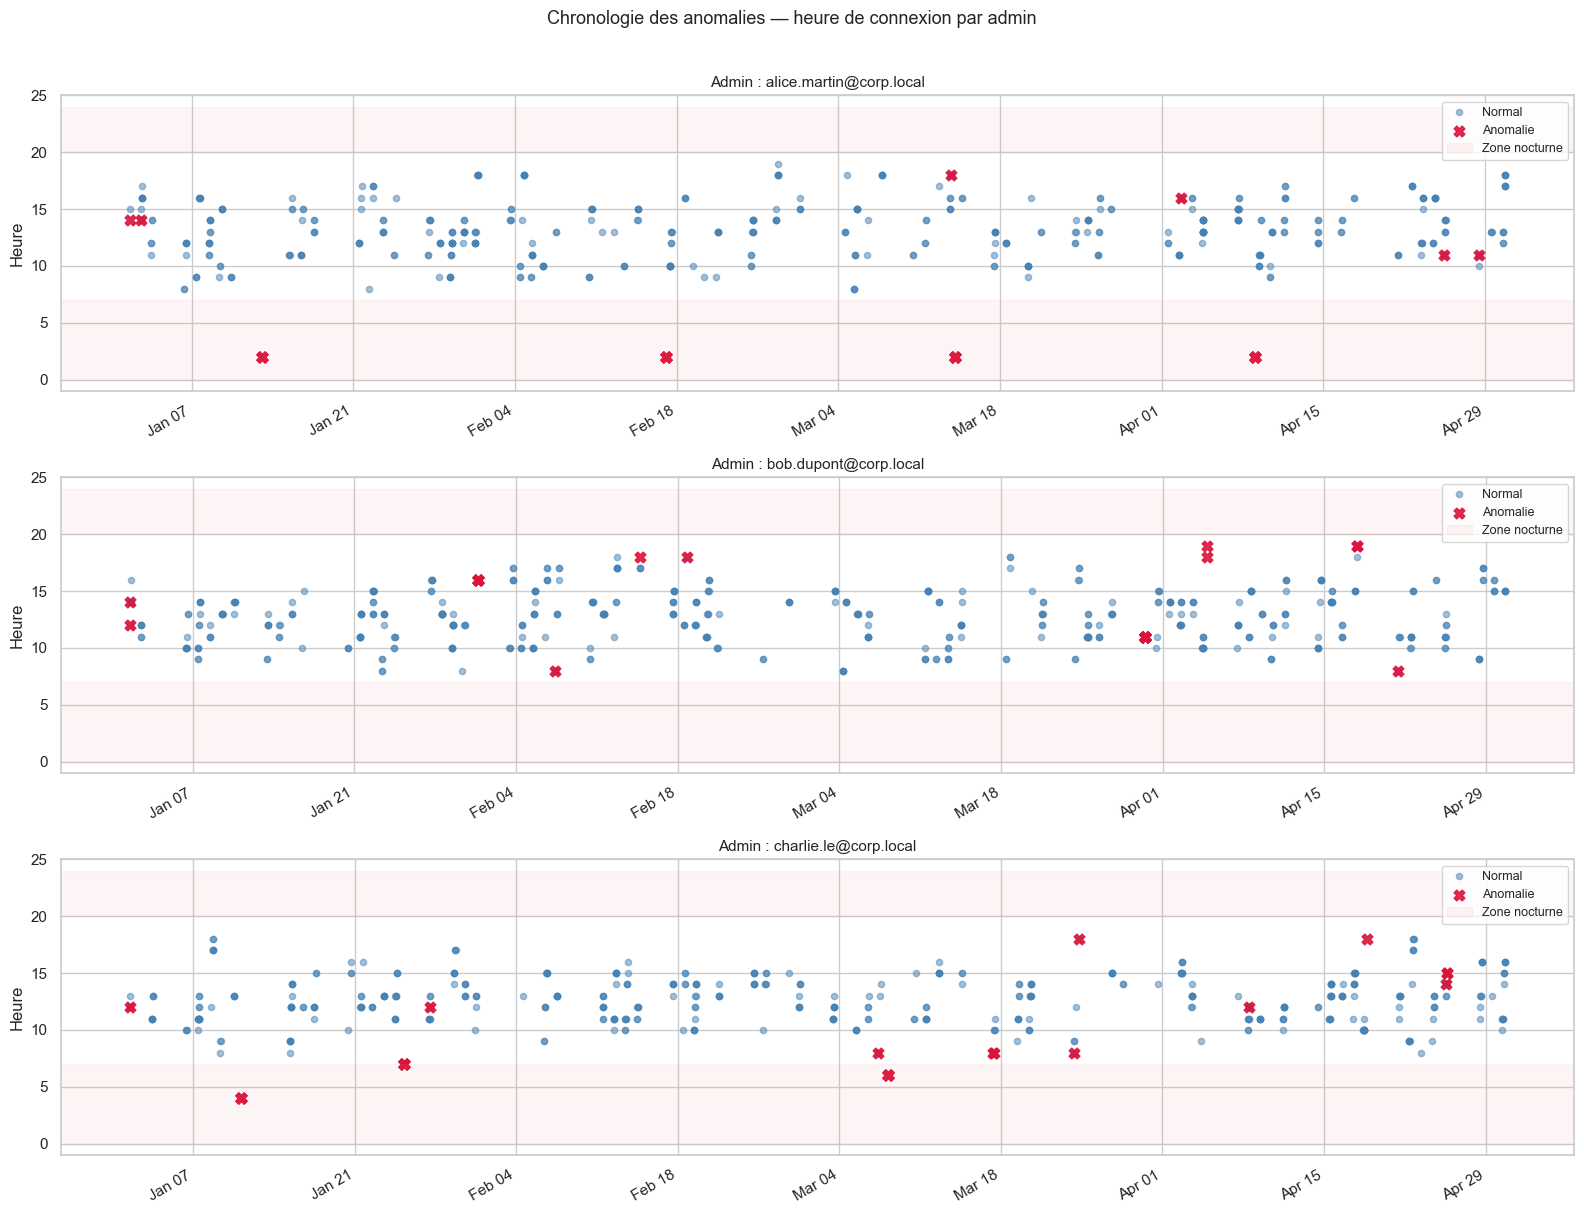
\includegraphics[width=0.98\textwidth]{images/Chronologie des anomalies par admin.png}
	
	\caption{Chronologie des événements administrateur avec points normaux et anomalies détectées. Objectif: vérifier visuellement la cohérence temporelle des alertes par rapport aux habitudes de connexion de chaque administrateur.}
	\label{fig:chronologie_anomalies_admin}
\end{figure}

Lecture: les marqueurs anormaux situés en dehors des plages horaires habituelles (nuit/week-end) sont priorisés pour investigation.

\subsubsection{Heatmap: Score d'anomalie par (jour, heure)}

\begin{figure}[H]
	\centering
		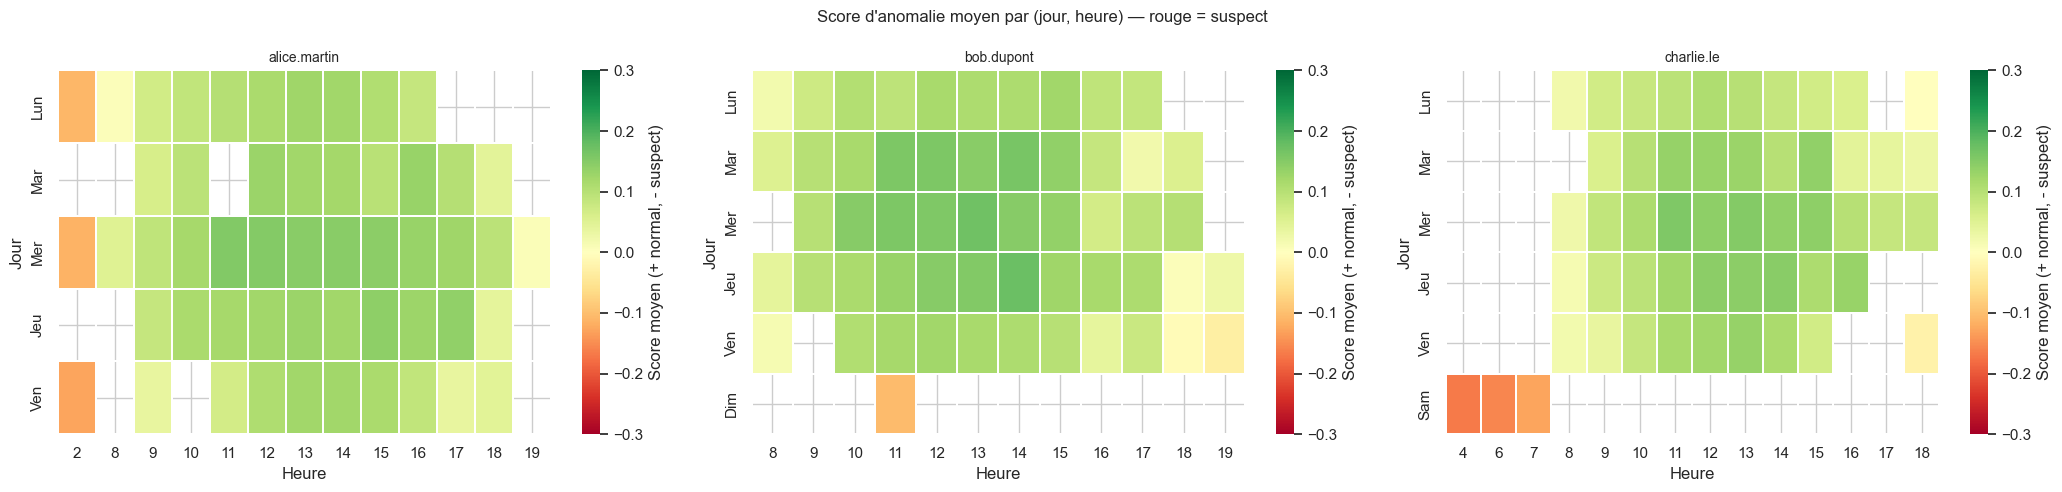
\includegraphics[width=0.98\textwidth]{images/Heatmapscoredanomaliemoyenparheure et jour de la semaine.png}
	
	\caption{Heatmap du score d'anomalie moyen par jour et par heure. Objectif: identifier les zones temporelles à risque où le comportement administrateur s'écarte du profil habituel.}
	\label{fig:heatmap_score_anomalie_admin}
\end{figure}

Lecture: les cellules rouges indiquent des créneaux atypiques et servent à orienter le réglage des seuils de détection.

\subsubsection{Distribution: Nouvelles IP vs anomalies}

\begin{figure}[H]
	\centering
		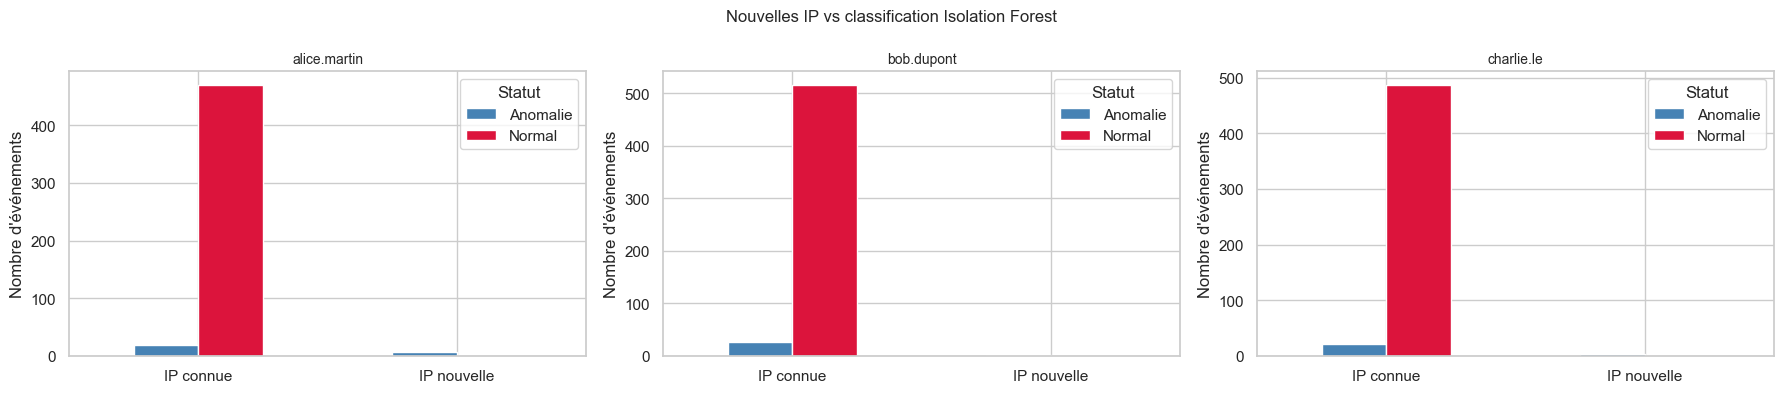
\includegraphics[width=0.98\textwidth]{images/Nouvelles IP vs classification Isolation Forest.png}
	
	\caption{Comparaison entre événements provenant d'IP connues et d'IP nouvelles, selon la classe Normal/Anomalie. Objectif: mesurer la contribution de la nouveauté réseau au risque détecté.}
	\label{fig:nouvelles_ip_vs_anomalies}
\end{figure}

Lecture: une proportion élevée d'anomalies sur IP nouvelles valide la pertinence de la feature \texttt{is\_new\_ip\_for\_admin}.

\subsubsection{Détection de rafales d'approbations}

\begin{figure}[H]
	\centering
		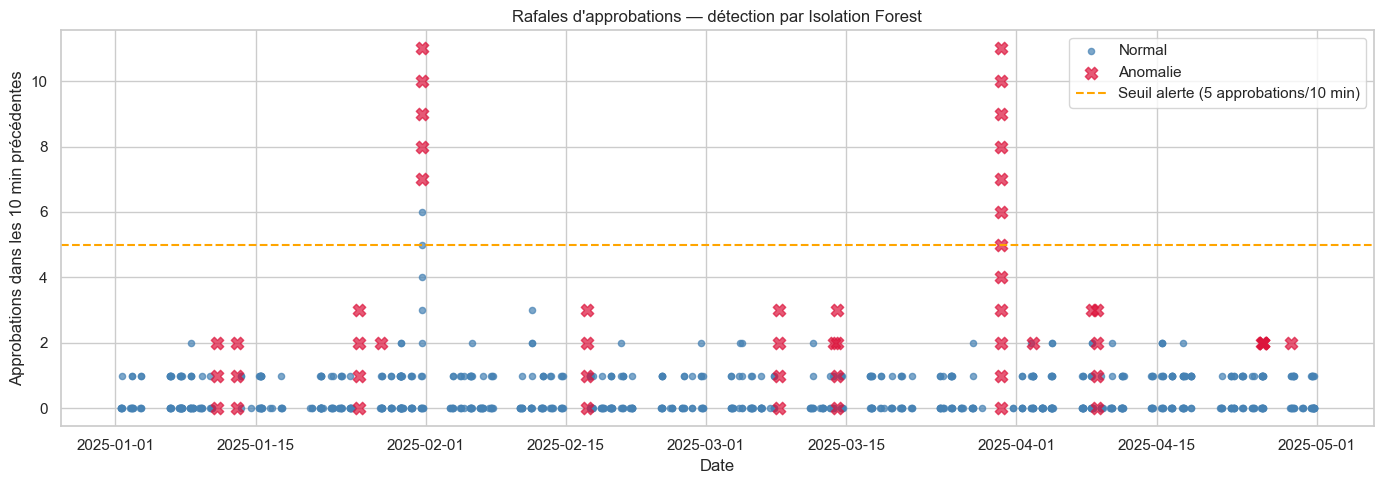
\includegraphics[width=0.98\textwidth]{images/Rafales approbations — détection par Isolation Forest.png}
	
	\caption{Détection des rafales d'approbations sur fenêtre glissante de 10 minutes. Objectif: distinguer l'activité opérationnelle normale des pics d'approbation potentiellement malveillants.}
	\label{fig:rafales_approbations_isolation_forest}
\end{figure}

Lecture: les points anormaux au-dessus du seuil opérationnel (5 approbations/10 min) déclenchent une alerte prioritaire.


\section{Intégration dans le workflow d'approbation JIT}

\subsection{Étape supplémentaire: Vérification d'approbateur}

Le moteur JIT applique maintenant une étape intermédiaire avant validation:

\begin{enumerate}
	\item Utilisateur demande accès $\rightarrow$ état \texttt{pending}.
	
	\item Système sélectionne un approbateur compatible.
	
	\item Moteur de détection d'anomalies évalue l'approbateur en temps réel:
	\begin{itemize}
		\item Si score d'anomalie $> 0.8$: l'approbateur est lui-même suspect. La demande est escaladée à un niveau supérieur ou rejetée.
		\item Si $0.6 < $ score $\leq 0.8$: Approbation possible, mais avec alertes SIEM amplifiées et audit renforcé.
		\item Si score $\leq 0.6$: Approbation autorisée normalement.
	\end{itemize}
	
	\item Approbateur approuve (ou refuse) normalement.
	
	\item Moteur JIT active l'accès et enregistre l'approbateur +  score d'anomalie pour audit ultérieur.
\end{enumerate}

\subsection{Tableau de bord de monitoring}

Le tableau de bord de sécurité affiche:

\begin{table}[h]
\centering
\begin{tabularx}{\textwidth}{|l|l|l|p{5cm}|}
\hline
\textbf{Admin} & \textbf{Score Anomalie (7j)} & \textbf{État} & \textbf{Action} \\
\hline
alice.martin@corp.local & 0.15 & ✓ Normal & - \\
\hline
bob.dupont@corp.local & 0.65 & ⚠ Borderline & Enquête suggérée \\
\hline
charlie.le@corp.local & 0.92 & ✗ Anomalie & Compte suspendu, escalade de sécurité \\
\hline
\end{tabularx}
\caption{Exemple de tableau de bord SOC pour le suivi des comptes privilégiés. Objectif: prioriser la réponse sécurité selon le score d'anomalie et le niveau de risque associé.}
\label{tab:dashboard_anomalies_admin}
\end{table}

\section{Cas d'usage et scénarios}

\subsection{Scénario 1: Compte compromis détecté}

\begin{itemize}
	\item Attaquant gagne accès au compte d'admin Bob via phishing.
	\item Entre 2h-4h du matin (heure attaquant en Asie), lance 30 demandes d'accès en rafale.
	\item Isolation Forest détecte: score anomalie de Bob passe de 0.2 à 0.85 en une nuit.
	\item Alerte SIEM: "Anomalie détectée - Admin Bob - Accès hors horaires habituels".
	\item Équipe sécurité reçoit notification. Enquête: IP de l'attaquant tracée, compte Bob forcé en déconnexion, MFA reconfigurée.
	\item Dommage limité: accès JIT n'a pu être approuvé que 3 fois avant la détection.
\end{itemize}

\subsection{Scénario 2: Privilèges escaladés abusivement}

\begin{itemize}
	\item Admin Alice (rôle standard) tente soudain d'approuver accès pour machines "critiques" (en-dehors de sa portée).
	\item Moteur JIT refuse l'approbation (contrôle RBAC); Isolation Forest marque la tentative comme anomalie.
	\item Alerte: "Escalade de privilèges tentée par Alice".
	\item Enquête révèle qu'Alice a un script malveillant qui tente d'élargir ses permissions.
\end{itemize}

\subsection{Scénario 3: Comportement acceptable mais inhabituel}

\begin{itemize}
	\item Admin Charlie travaille habituellement 9h-17h.
	\item Projet urgent survient; travail nocturne (22h-6h) pendant 5 jours.
	\item Isolation Forest détecte anomalie (score 0.72).
	\item Équipe sécurité valide le contexte auprès de Charlie: Projet X, justification acceptable.
	\item Faux positif reconnu; seuil affiné ou exception documentée.
\end{itemize}

\section{Ajustement et tuning du modèle}

\subsection{Paramètre \texttt{contamination}}

Le paramètre \texttt{contamination} définit le pourcentage d'observations attendues comme anomalies.
Il influence directement la sensibilité du modèle:

\begin{itemize}
	\item \textbf{contamination = 0.02}: Très strict. Suppose 2\% d'anomalies. Peu d'alertes, risque de faux négatifs (manquer les attaques).
	
	\item \textbf{contamination = 0.05}: Recommandé pour PME. Suppose 5\% d'anomalies. Équilibre sensibilité/faux positifs.
	
	\item \textbf{contamination = 0.10}: Permissif. Suppose 10\% d'anomalies. Plus d'alertes, meilleure couverture.
	
	\item \textbf{contamination = 0.20}: Très sensible. Suppose 20\% d'anomalies. Beaucoup de faux positifs.
\end{itemize}

Ajustement recommandé selon contexte:
\begin{itemize}
	\item \textbf{PME sans historique incident}: contamination = 0.05.
	\item \textbf{PME avec quelques incidents}: contamination = 0.05–0.10.
	\item \textbf{Secteur finance/santé/critique}: contamination = 0.02–0.05 (très strict).
\end{itemize}

\subsection{Fenêtre temporelle d'apprentissage}

Le modèle s'entraîne sur des données historiques. Le choix de la fenêtre affecte l'adaptabilité:

\begin{itemize}
	\item \textbf{7 jours}: Capture variations semaine-type. Rapide, réactif aux changements. \textbf{Recommandé au démarrage}.
	
	\item \textbf{14 jours}: Captures 2 semaines = fériés, projets courts. Meilleur équilibre.
	
	\item \textbf{30 jours}: Captures variations mensuelles, congés. Modèle plus stable mais lent à s'adapter aux changements.
	
	\item \textbf{90 jours}: Captures saisonnalité. Très stable mais peu réactif; risque d'oublier nouvelles règles.
\end{itemize}

Recommandation: Démarrer avec 7-14 jours, évaluer faux positifs/négatifs après 2-3 semaines, allonger si stabilité insuffisante.

\subsection{Seuil d'alerte}

Le score d'anomalie varie de 0 (normal) à 1 (fortement anormal). Le seuil détermine quand déclencher une alerte:

\begin{itemize}
	\item \textbf{Seuil $t = 0.80$}: Très strict. Seules les anomalies fortes ($A(x) > 0.80$) déclenchent alerte.
	
	\item \textbf{Seuil $t = 0.70$}: Équilibré (recommandé). Entre normal et attention.
	
	\item \textbf{Seuil $t = 0.60$}: Sensible. Capture anomalies moyennes aussi.
	
	\item \textbf{Seuil $t = 0.50$}: Très sensible. Tout ce qui s'écarte du "très normal" trigger alerte.
\end{itemize}

À tester et affiner en fonction du volume d'alertes et faux positifs observés.

\subsubsection{Approche progressive}

\begin{enumerate}
	\item Démarrer avec seuil 0.75 (très strict).
	\item Observer pendant 1 mois.
	\item Si trop peu d'alertes: réduire à 0.70 ou 0.60.
	\item Si trop de faux positifs: augmenter à 0.80.
	\item Documenter les seuils ajustés et les raisons.
\end{enumerate}

\section{Limitations et considérations}

\subsection{Problème du cold start}

Lors du démarrage du système, \textbf{toute IP est "nouvelle"} pour chaque administrateur, car aucun historique 30-jours n'existe.

\textbf{Mitigation}:
\begin{itemize}
	\item Réduire la période lookback lors des premières semaines (ex: 5 jours au lieu de 30).
	\item Ignorer ou pondérer moins fortement \texttt{is\_new\_ip\_for\_admin} pendant les 2 premières semaines.
	\item Laisser tourner le système en mode "debug" (alertes non-bloquantes) pendant 30 jours avant production.
\end{itemize}

\subsection{Faux positifs: Comportements légitimes inhabituels}

Isolation Forest peut flaguer comme anormal:
\begin{itemize}
	\item \textbf{Projet d'urgence}: Travail nocturne nécessaire (est marqué "is\_night"=1 $\Rightarrow$ anomalie).
	\item \textbf{Télétravail soudain}: IP change (est marqué "is\_new\_ip"=1 $\Rightarrow$ anomalie).
	\item \textbf{Changement de rôle}: Nouvel admin hérite habits différents (débute zéro historique).
	\item \textbf{Congé suivi de surcharge}: Pic d'activités post-vacances (approvals\_last\_10min élevé).
\end{itemize}

\textbf{Mitigation}:
\begin{itemize}
	\item Documenter exceptions approuvées (ex: "Alice = télétravail définitif depuis 15/03/2025").
	\item Implémenter système de \textit{whitelist} d'IPs ou heures spéciales pour chaque admin.
	\item Utiliser 2 seuils: $t_{\text{strict}}=0.80$ (alerte immédiate) et $t_{\text{warning}}=0.60$ (inspection manuelle).
	\item Créer un tableau de bord pour SecurityOps: réviser les 10 principales anomalies par mois, puis valider ou rejeter.
\end{itemize}

\subsection{Concept Drift (dérive de concept)}

Le comportement normal d'un admin peut se modifier graduellement:
\begin{itemize}
	\item Télétravail permanent (IP change).
	\item Promotion vers rôle avec horaires décalés (heure change).
	\item Changements saisonniers (moins d'approbations en été).
\end{itemize}

Ce qui était anomalie hier devient normal aujourd'hui.

\textbf{Mitigation}:
\begin{itemize}
	\item \textbf{Réentraînement régulier}: réentraîner le modèle de manière hebdomadaire ou mensuelle.
	\item \textbf{Fenêtre glissante}: Utiliser "rolling window" des 30 derniers jours (pas figé).
	\item \textbf{Feedback loop}: Si alerte marquée "faux positif" par SecurityOps, intégrer dans données futures.
	\item \textbf{Monitoring du drift}: Tracker "score moyen par admin" — si hausse progressive = concept drift détecté.
\end{itemize}

\subsection{Comptes de service et bots}

Les comptes de service (intégrations, jobs cron, robots) ont des patterns totalement différents:
\begin{itemize}
	\item Connexions à \textbf{heures fixes} (00:05, 12:15 précisément).
	\item \textbf{Très fréquentes} (1000+ par jour) $\Rightarrow$ \texttt{approvals\_last\_10min} toujours élevé.
	\item De \textbf{mêmes IPs} (pas d'IP nouvelles).
	\item Pas de concept "jour/nuit" ou "week-end".
\end{itemize}

Entraîner Isolation Forest sur ces comptes produirait alertes inutiles.

\textbf{Mitigation}:
\begin{itemize}
	\item Créer \textbf{modèles séparés}: un pour "admins humains", un pour "service accounts".
	\item Ou exclure entièrement service accounts de cette détection (ils relèvent d'autres contrôles).
	\item Tagguer les comptes en fonction de type (attribut "account\_type" = "human" ou "bot").
\end{itemize}

\subsection{Données manquantes ou corrompues}

Si logs Wazuh Indexer sont incomplets (dépôt échoué, agent down), features seront biaisées.

\textbf{Mitigation}:
\begin{itemize}
	\item Checker santé agents Wazuh avant extraction.
	\item Ignorer jours avec < 50\% data pour admin (données insuffisantes).
	\item Implémenter alerte "données manquantes pour admin X" $\Rightarrow$ détection temporairement désactivée pour X.
\end{itemize}

\subsection{Respect de la vie privée (RGPD)}

Collecter et analyser logs d'administrateur soulève questions RGPD:
\begin{itemize}
	\item \textbf{Légal}: Les administrateurs doivent consentir ou avoir justification légitime (sécurité).
	\item \textbf{Transparence}: Communication claire que surveillance effectuée.
	\item \textbf{Rétention}: Combien de temps conserver les logs? (Recommandation: 90 jours max).
	\item \textbf{Accès}: Qui peut voir les alertes? (responsables sécurité).
\end{itemize}

\textbf{Mitigation}:
\begin{itemize}
	\item Documenter base légale dans politique de sécurité.
	\item Chiffrer logs et alertes en transit/repos.
	\item Implémenter contrôle d'accès (RBAC) sur dashboard anomalies.
	\item Archiver et supprimer logs après rétention.
\end{itemize}

\section{Conclusion du chapitre}

La détection d'anomalies appliquée aux administrateurs répond à la question critique \textit{"Qui garde les gardiens?"} 
en mettant en place une \textbf{surveillance comportementale continue basée sur les données réelles} provenant de Wazuh Indexer.

\subsection{Pipeline complet}

Le système fonctionne selon ce processus:

\begin{enumerate}
	\item \textbf{Collecte}: Agents Wazuh sur chaque service (Authentik, moteur JIT, SSH) envoient logs au Wazuh Manager.
	
	\item \textbf{Centralisation}: Wazuh Indexer (OpenSearch/Elasticsearch) centralise et indexe tous les logs.
	
	\item \textbf{Extraction}: Script Python récupère les logs administrateur via requêtes API Wazuh (dernières 7-30 jours).
	
	\item \textbf{Feature engineering}: Calcul de 8 features comportementales (heure, jour, IP nouvelle, rafales, etc.).
	
	\item \textbf{Détection ML}: Isolation Forest entraîné par admin détecte anomalies (score 0-1).
	
	\item \textbf{Alertes}: Scores > 0.60-0.75 génèrent custom alerts dans Wazuh + notifications SecurityOps.
	
	\item \textbf{Décision JIT}: Avant d'approuver une demande d'accès, le moteur JIT consulte le score d'anomalie 
	du demandeur $\Rightarrow$ peut refuser ou escalader si approbateur lui-même suspect.
	
	\item \textbf{Audit}: Tous les scores d'anomalie sont loggés pour audit/historique (traçabilité complète).
	
	\item \textbf{Feedback}: SecurityOps valide alertes; faux positifs $\Rightarrow$ raffinement modèle.
\end{enumerate}

\subsection{Avantages de cette approche}

\begin{itemize}
	\item \textbf{Données réelles}: Basé sur logs vrais provenant de Wazuh, pas synthétiques.
	
	\item \textbf{Non-supervisé}: Pas besoin d'étiqueter "normal" vs. "anormal" manuellement.
	
	\item \textbf{Modèles individuels}: Un profil par admin $\Rightarrow$ détecte écarts personnels.
	
	\item \textbf{Interprétable}: Isolation Forest fournit features explicatives (pourquoi flagué).
	
	\item \textbf{Léger}: Exécutable sur ressources limitées (cron job sur serveur sécurité).
	
	\item \textbf{Zero Trust}: Couvre la boucle complète: même les administrateurs restent sous surveillance.
\end{itemize}

\subsection{Métriques de succès}

Après déploiement, tracker:

\begin{itemize}
	\item \textbf{Taux de détection}: Combien d'anomalies réelles (comptes compromis) détectées avant dommage?
	
	\item \textbf{Faux positifs}: Combien d'alertes invalides par mois? (Cible: < 10\%).
	
	\item \textbf{MTTR (Mean Time To Response)}: Temps entre alerte et action SecurityOps (Cible: < 30 min).
	
	\item \textbf{Stabilité modèle}: Score moyen/écart-type par admin stable ou dérives?
	
	\item \textbf{Couverture}: Quel \% d'admins ont au moins 10 logs/jour pour entraînement fiable?
\end{itemize}

\subsection{Perspectives d'amélioration}

\begin{enumerate}
	\item \textbf{Enrichissement IP}: Ajouter résolution GeoIP (pays, ASN) pour détecter changements géo impossibles.
	
	\item \textbf{Corrélation multi-événements}: Lier anomalies d'admin à alertes parallèles (ex: approbation anormale + tentative privilège escalade sur machine).
	
	\item \textbf{Modèles supervisés hybrides}: Si suffisante données labelisées, combiner Isolation Forest + modèles supervisés (RandomForest, XGBoost).
	
	\item \textbf{Apprentissage par renforcement}: Système qui apprend du feedback SecurityOps en temps réel.
	
	\item \textbf{Graphes de comportement}: Représenter les admins et leurs interactions (qui approuve qui, qui peut accéder où) en tant que graphe; détection d'anomalies sur graphes (Graph Neural Networks).
\end{enumerate}

\subsection{Résumé}

En combinant collecte centralisée (Wazuh), ingénierie de features comportementales, Isolation Forest ML, 
et intégration JIT, nous établissons un système robuste de détection des anomalies administrateur. 

Cette approche transforme la gestion des administrateurs d'une \textit{position de confiance implicite} 
à un modèle \textit{de vérification continue et automatisée}, aligné pleinement avec l'esprit \textbf{Zero Trust} du projet.
\chapterpage{Chapitre 5 : Implementation}
\chapter{Implementation par composant}

\section{Introduction du chapitre}
Ce chapitre decrit l'implementation concrete de chaque composant de l'architecture cible. L'objectif est de montrer comment les choix de conception sont traduits en configurations, en logique applicative et en mecanismes techniques verifiables.

\section{Authentik (IAM)}
Authentik constitue le point central de confiance de l'architecture.

Les elements implantes sont:
\begin{itemize}
	\item la gestion des utilisateurs et des groupes metier;
	\item la federation d'authentification pour les services integres;
	\item l'emission de claims (groupes, identifiant, email) consommes par l'application.
\end{itemize}

La sequence d'authentification observee dans le projet montre d'abord l'entree utilisateur dans Tailscale, puis la redirection vers Authentik, et enfin le retour vers Tailscale apres succes SSO.

\begin{figure}[H]
	\centering
	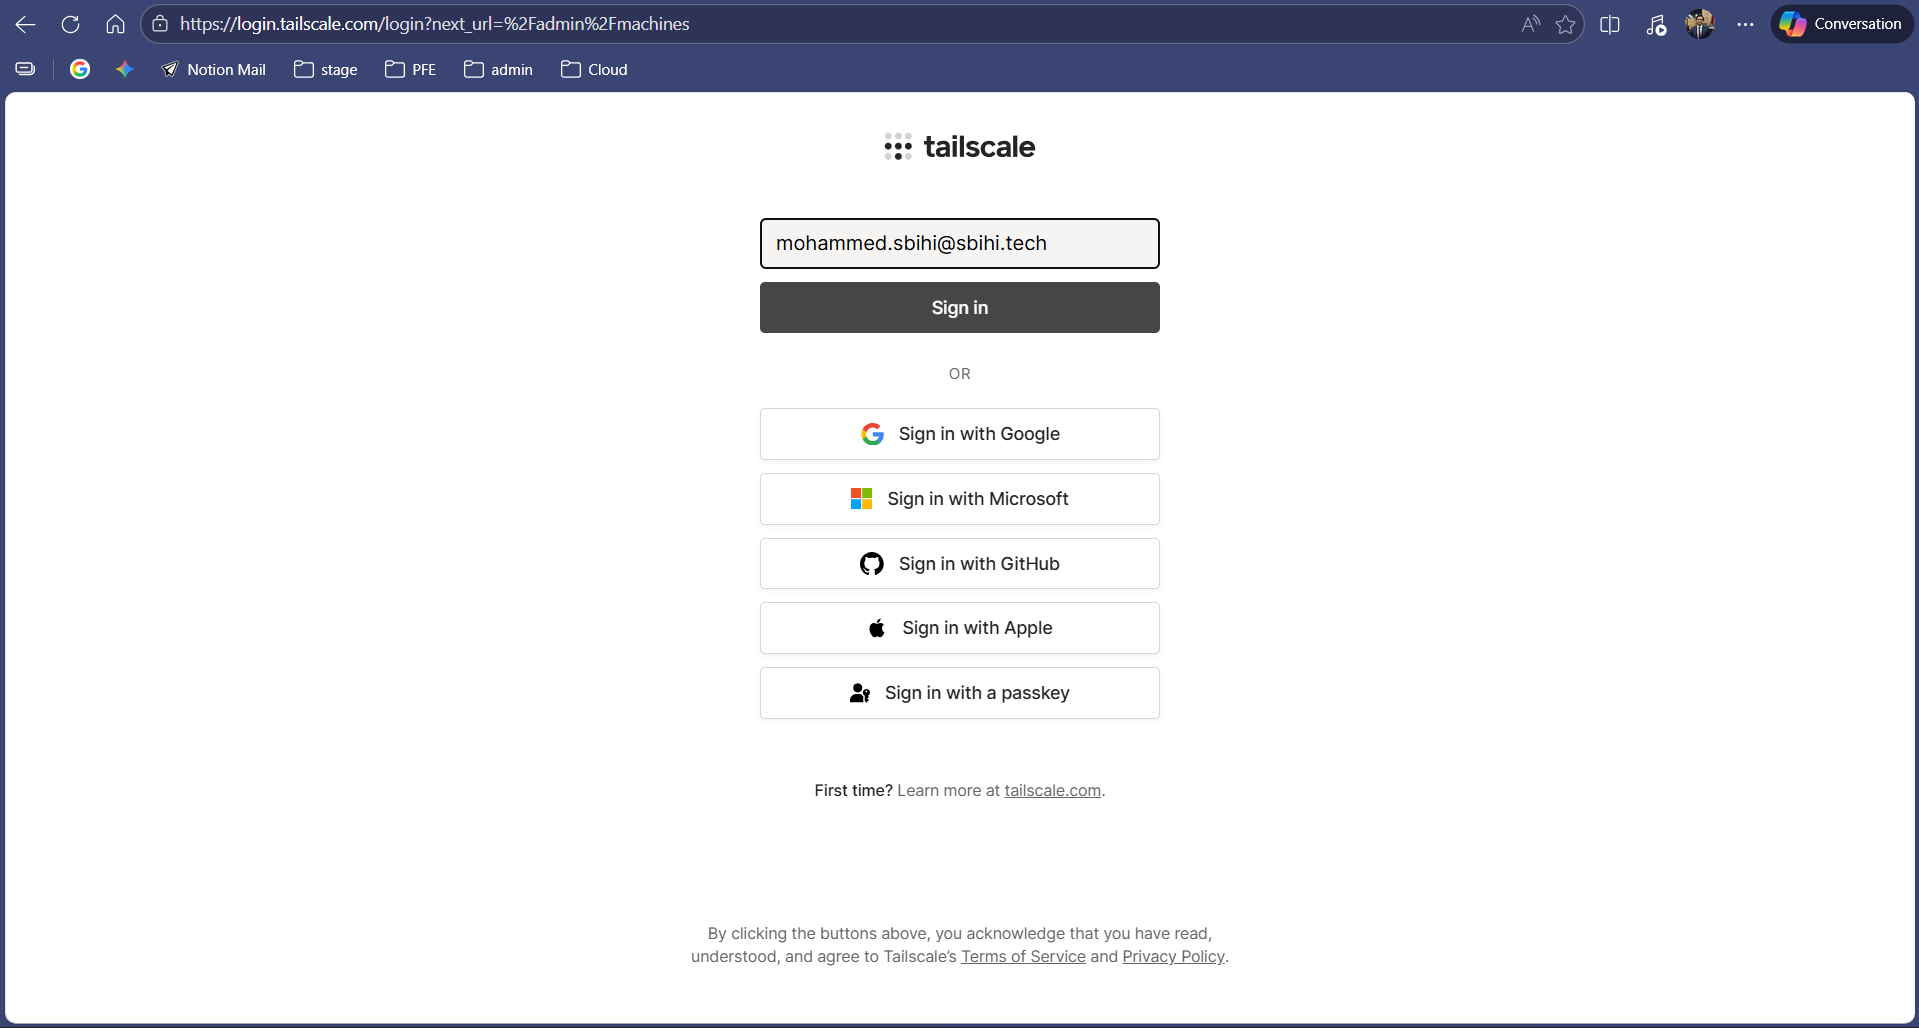
\includegraphics[width=0.82\textwidth]{images/tailscale_login/step1_enter_email.png}
	\caption{Etape 1: saisie de l'email utilisateur dans le flux de connexion Tailscale.}
	\label{fig:tailscale-step1-email}
\end{figure}
Cette ecran montre le point de depart du controle d'identite. L'utilisateur ne se connecte pas directement a la ressource cible: il initie d'abord un flux IAM, ce qui garantit que toute demande d'acces est rattachee a une identite explicite et tracable.

\begin{figure}[H]
	\centering
	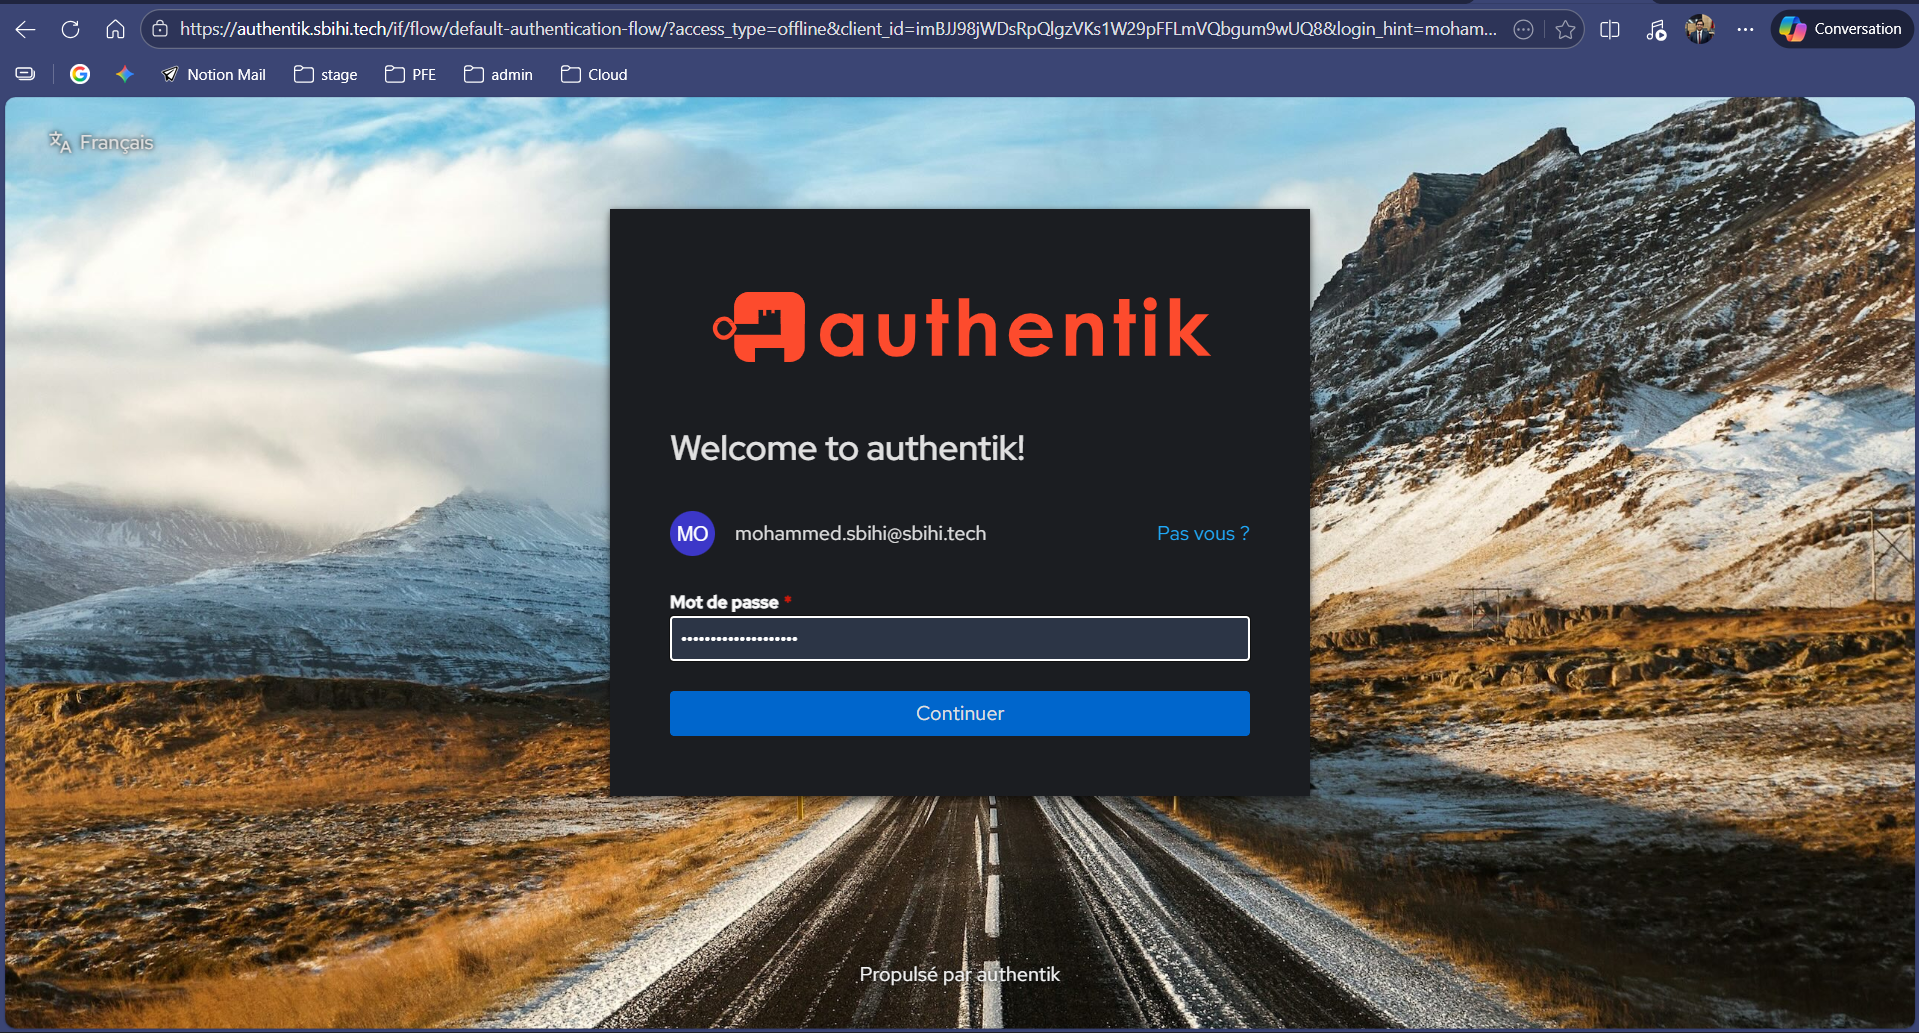
\includegraphics[width=0.82\textwidth]{images/tailscale_login/step2_rederection_to_authentik.png}
	\caption{Etape 2: redirection vers Authentik pour la verification d'identite (SSO IAM).}
	\label{fig:tailscale-step2-authentik}
\end{figure}
La redirection vers Authentik materialise la separation entre couche reseau et couche identite. Cette etape est essentielle dans Zero Trust, car la politique d'acces n'est appliquee qu'apres verification de l'identite et du contexte de connexion.

\begin{figure}[H]
	\centering
	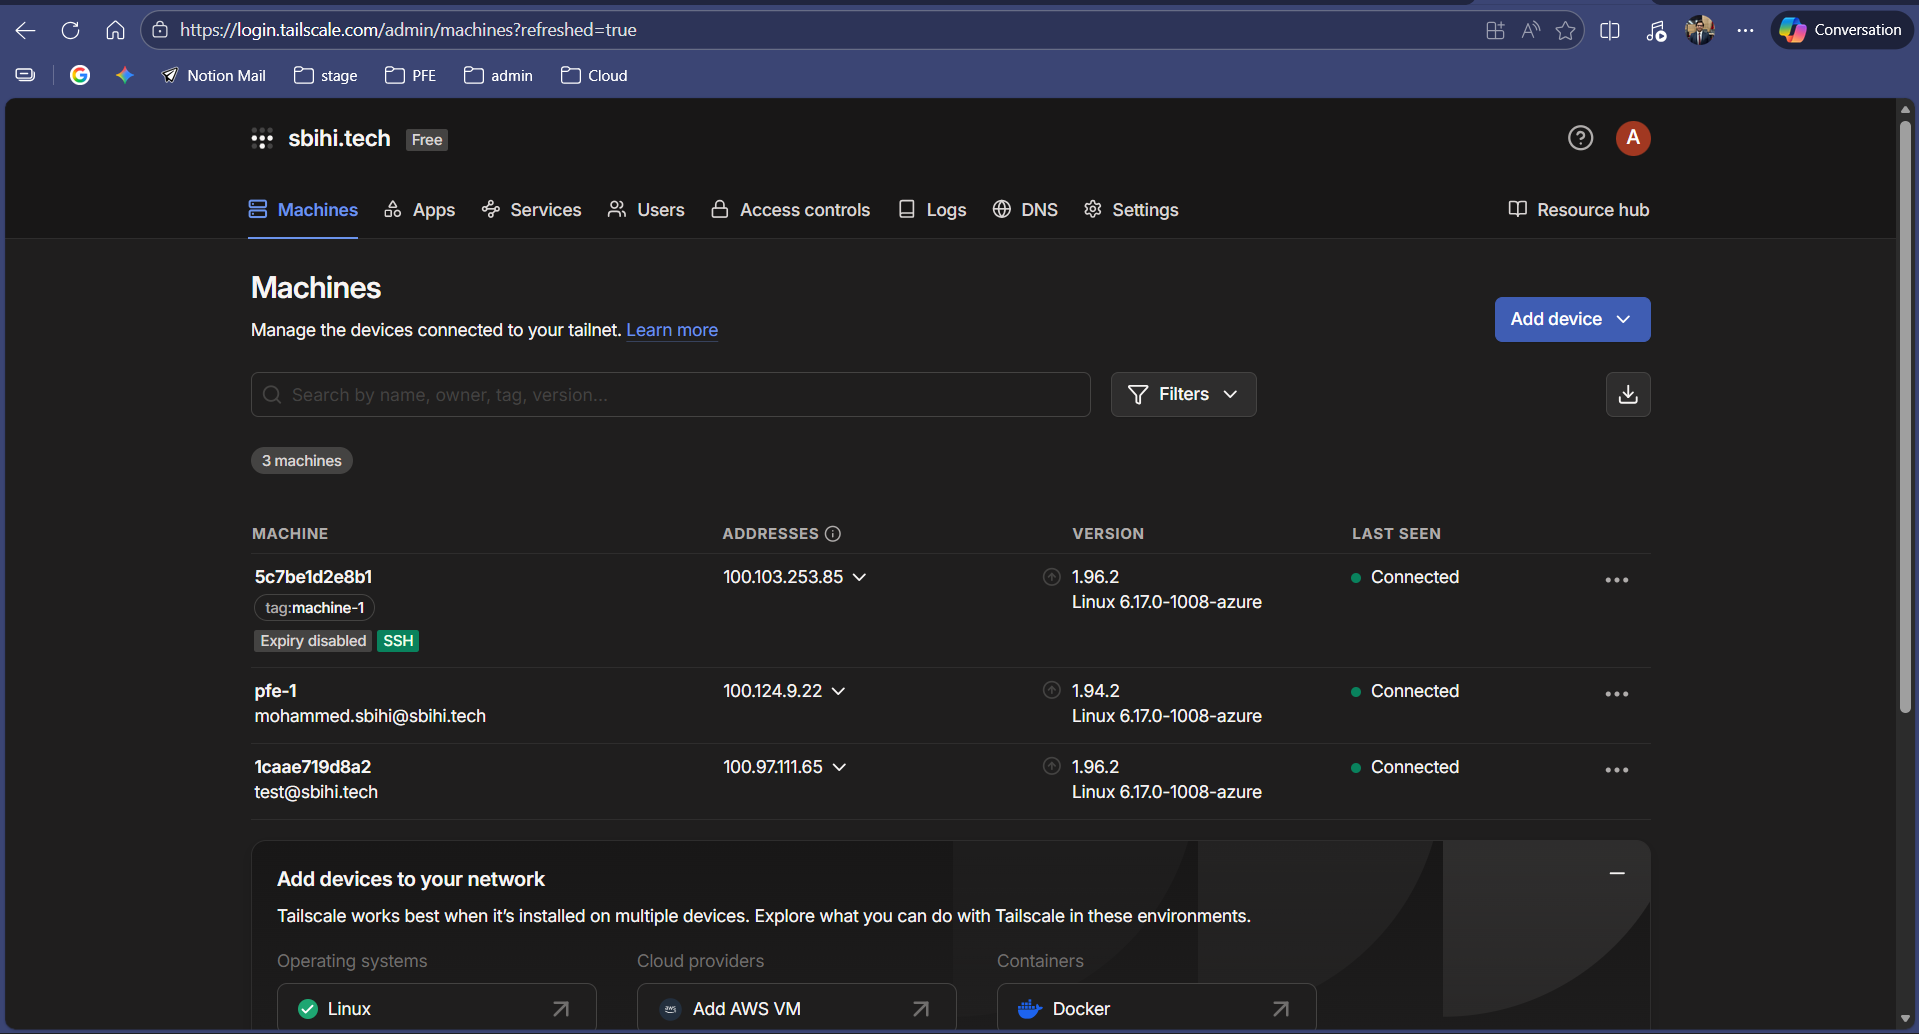
\includegraphics[width=0.82\textwidth]{images/tailscale_login/step3_back_to_tailscale.png}
	\caption{Etape 3: retour vers Tailscale apres authentification validee par Authentik.}
	\label{fig:tailscale-step3-back}
\end{figure}
Le retour vers Tailscale confirme que la federation d'authentification est correctement etablie. En pratique, cela permet de n'autoriser ensuite que les operations compatibles avec les droits du profil authentifie.

\begin{figure}[H]
	\centering
	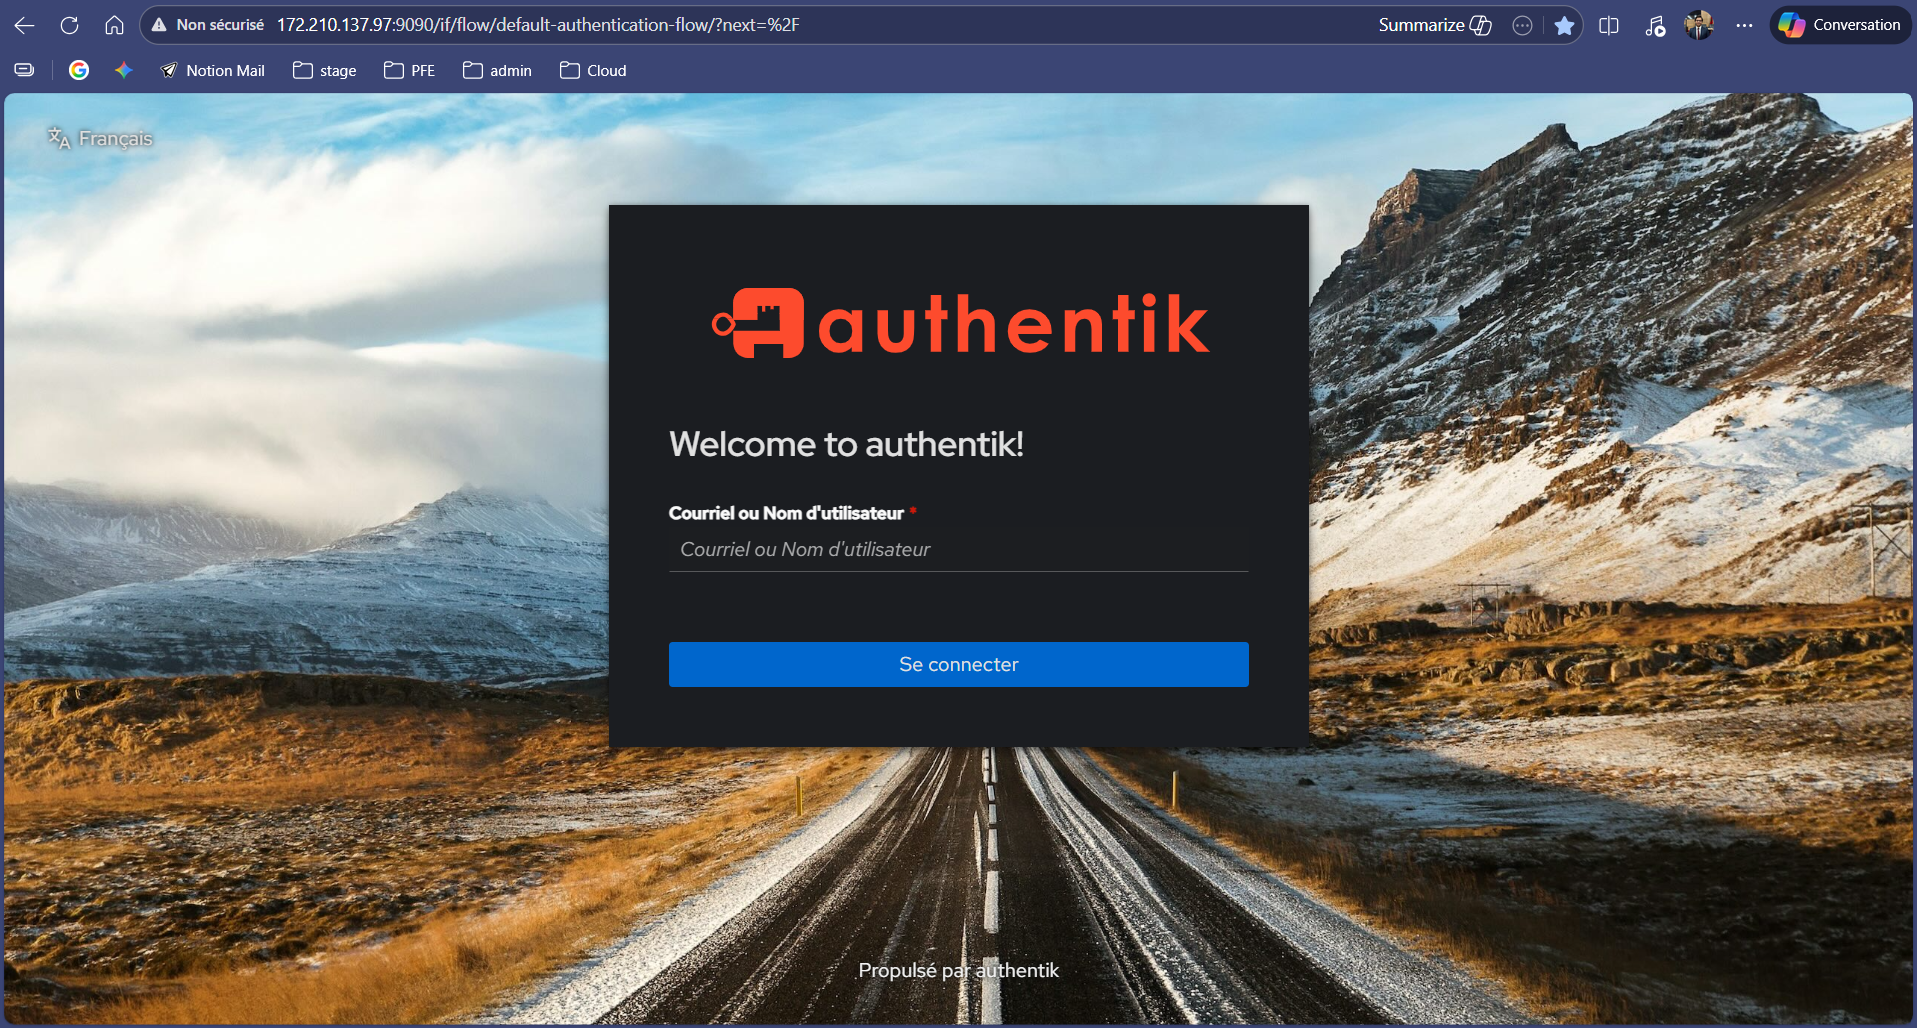
\includegraphics[width=0.9\textwidth]{images/capture de la page login.png}
	\caption{Page de connexion IAM de l'application, point d'entree du controle d'identite.}
	\label{fig:iam-login-page}
\end{figure}
Cette interface centralise l'authentification des utilisateurs de l'application de gouvernance JIT. Son role est de garantir que les actions metier (demande, approbation, revocation) sont executees par des comptes identifies et non anonymes.

\begin{figure}[H]
	\centering
	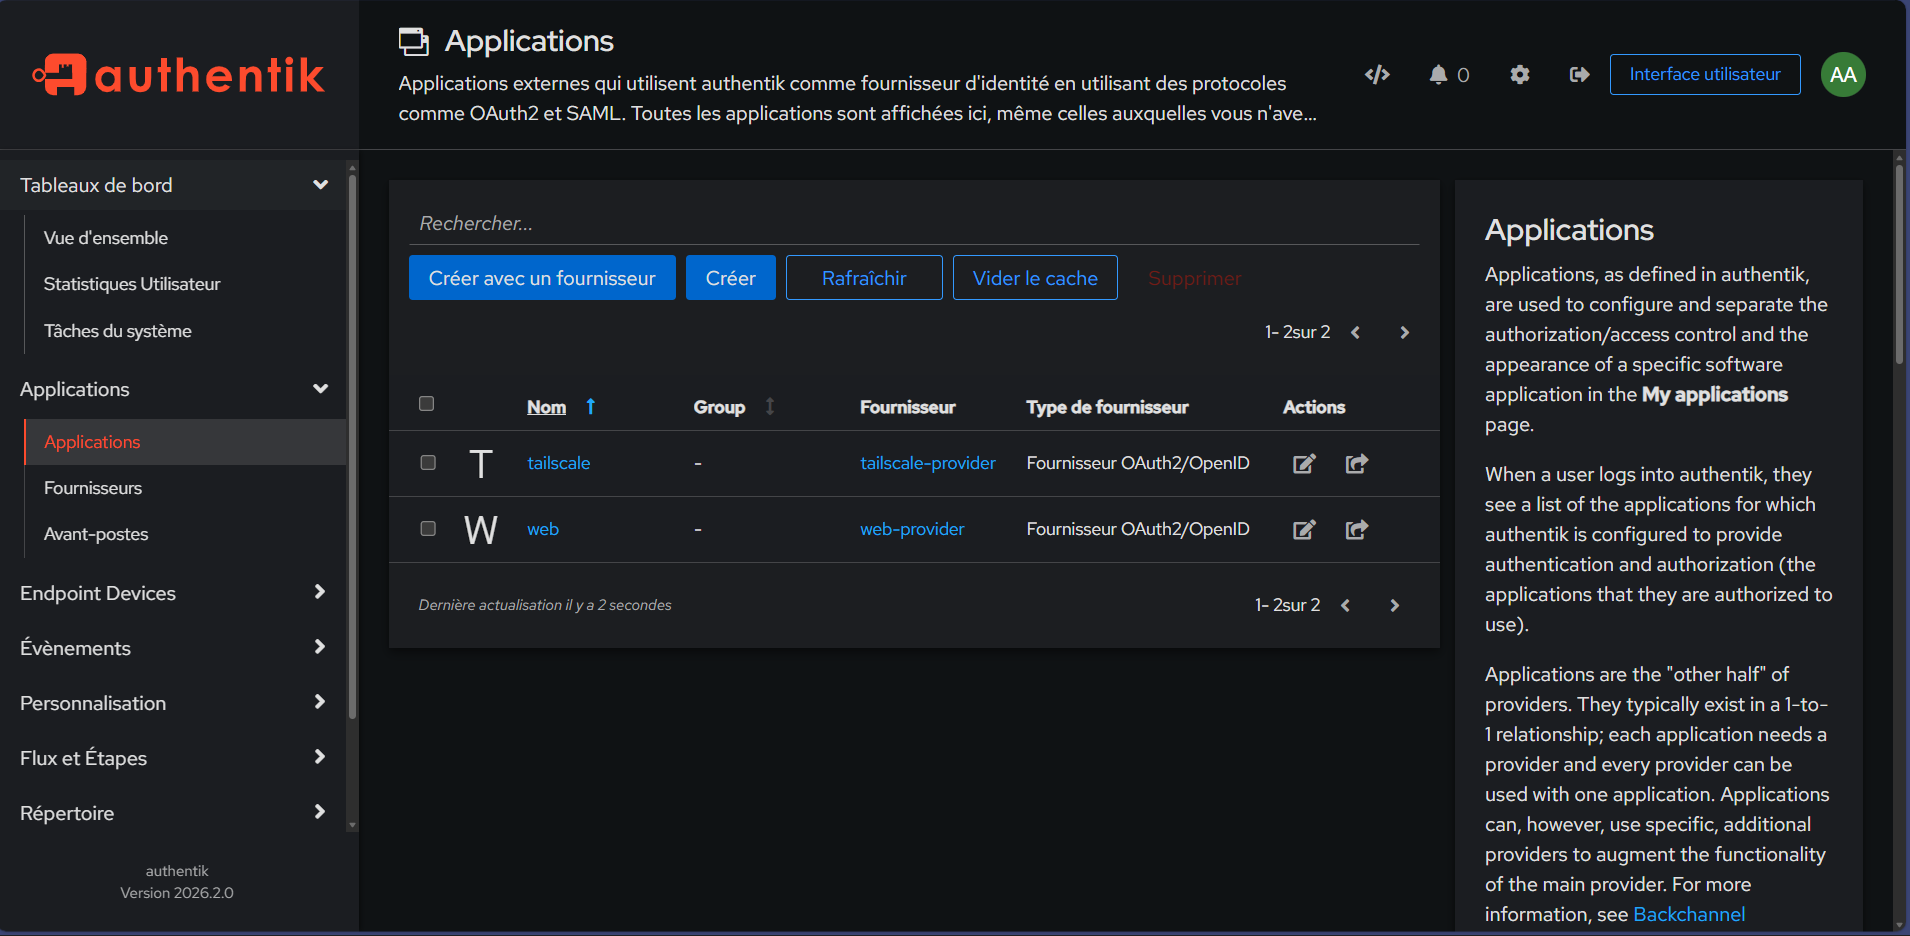
\includegraphics[width=0.9\textwidth]{images/capture de la configuration application.png}
	\caption{Configuration de l'application dans Authentik (provider, integration et parametres de federation).}
	\label{fig:iam-app-config}
\end{figure}
La configuration du provider est la piece technique qui relie le portail IAM a l'application Flask. Elle definit les URLs de redirection, les attributs transmis et les regles de confiance entre les deux systemes.

\begin{figure}[H]
	\centering
	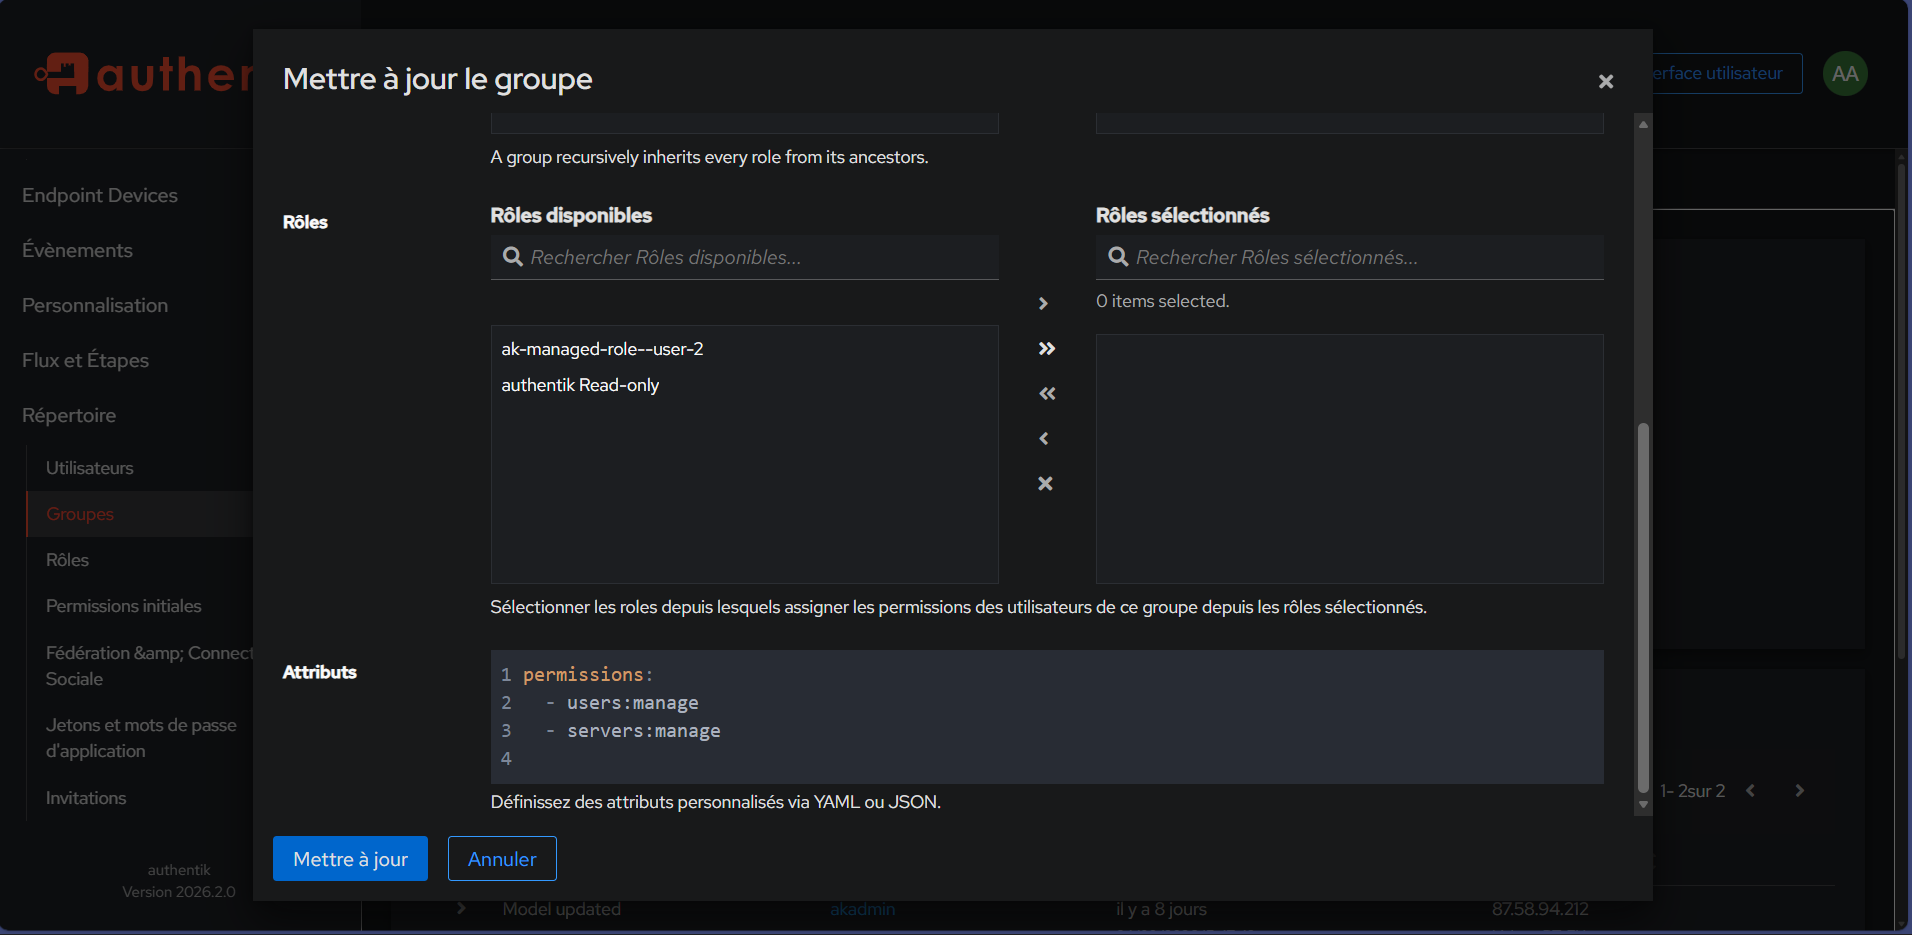
\includegraphics[width=0.9\textwidth]{images/groupes utilises pour la politique d'acces.png}
	\caption{Groupes utilises pour la politique d'acces et l'application des droits par profil.}
	\label{fig:iam-groups-policy}
\end{figure}
L'utilisation de groupes permet de decouper proprement les privileges entre utilisateurs standards et administrateurs. Ce modele facilite l'audit, car chaque droit peut etre justifie par l'appartenance a un groupe metier defini.

\section{Tailscale ACL (controle reseau)}
Tailscale est utilise comme couche de controle reseau Zero Trust avec ACL explicites.

Les points clefs de configuration sont:
\begin{itemize}
	\item etiquetage des machines cibles (tags d'environnement et de criticite);
	\item regles ACL fondees sur l'identite/groupe et la machine cible;
	\item ouverture d'acces strictement conditionnee a l'approbation JIT.
\end{itemize}

L'effet recherche est binaire et verifiable:
\begin{itemize}
	\item avant approbation JIT: acces refuse;
	\item apres approbation JIT: acces autorise pendant la fenetre TTL;
	\item apres expiration TTL: acces de nouveau refuse.
\end{itemize}

\begin{figure}[H]
	\centering
	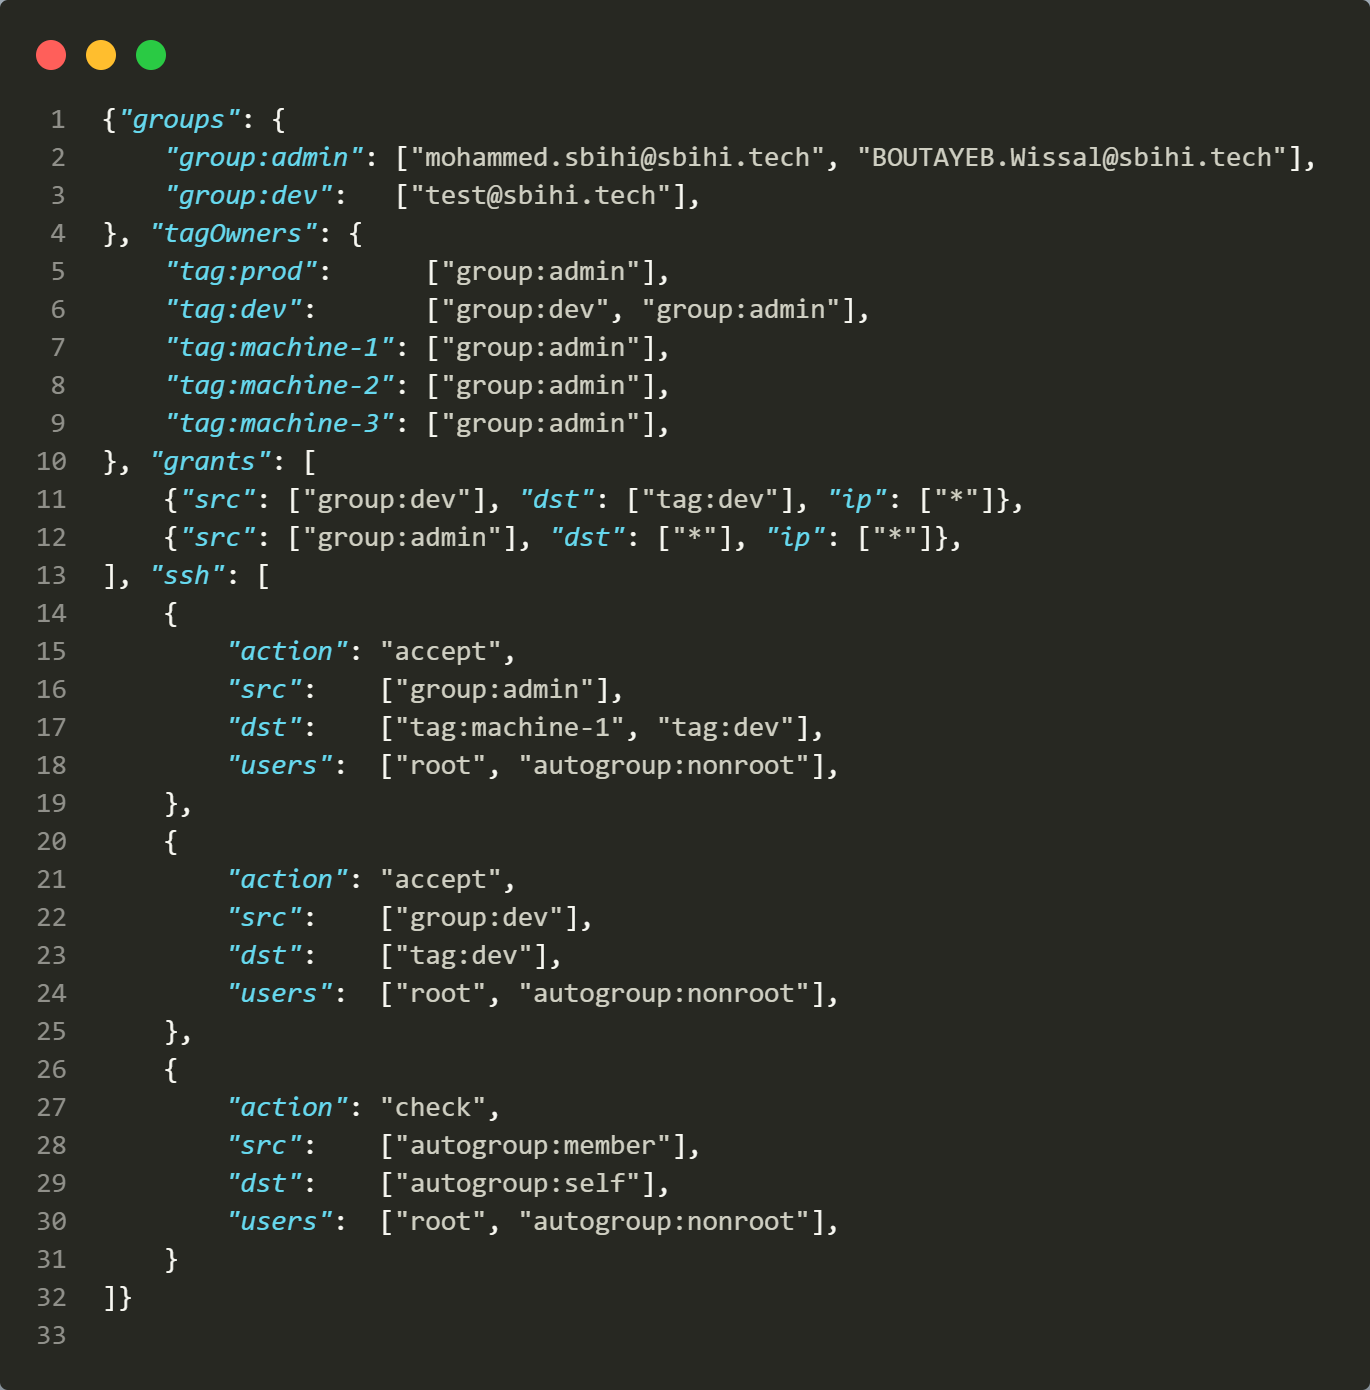
\includegraphics[width=0.95\textwidth]{images/acl-before-acces-granted.png}
	\caption{Etat ACL avant approbation: politique restrictive, sans autorisation explicite pour l'utilisateur cible.}
	\label{fig:acl-before-grant}
\end{figure}
Cette capture illustre le principe de base du modele Zero Trust: l'absence d'autorisation explicite equivaut a un refus d'acces. L'utilisateur ne peut donc pas atteindre la cible tant que la gouvernance JIT n'a pas valide la demande.

\begin{figure}[H]
	\centering
	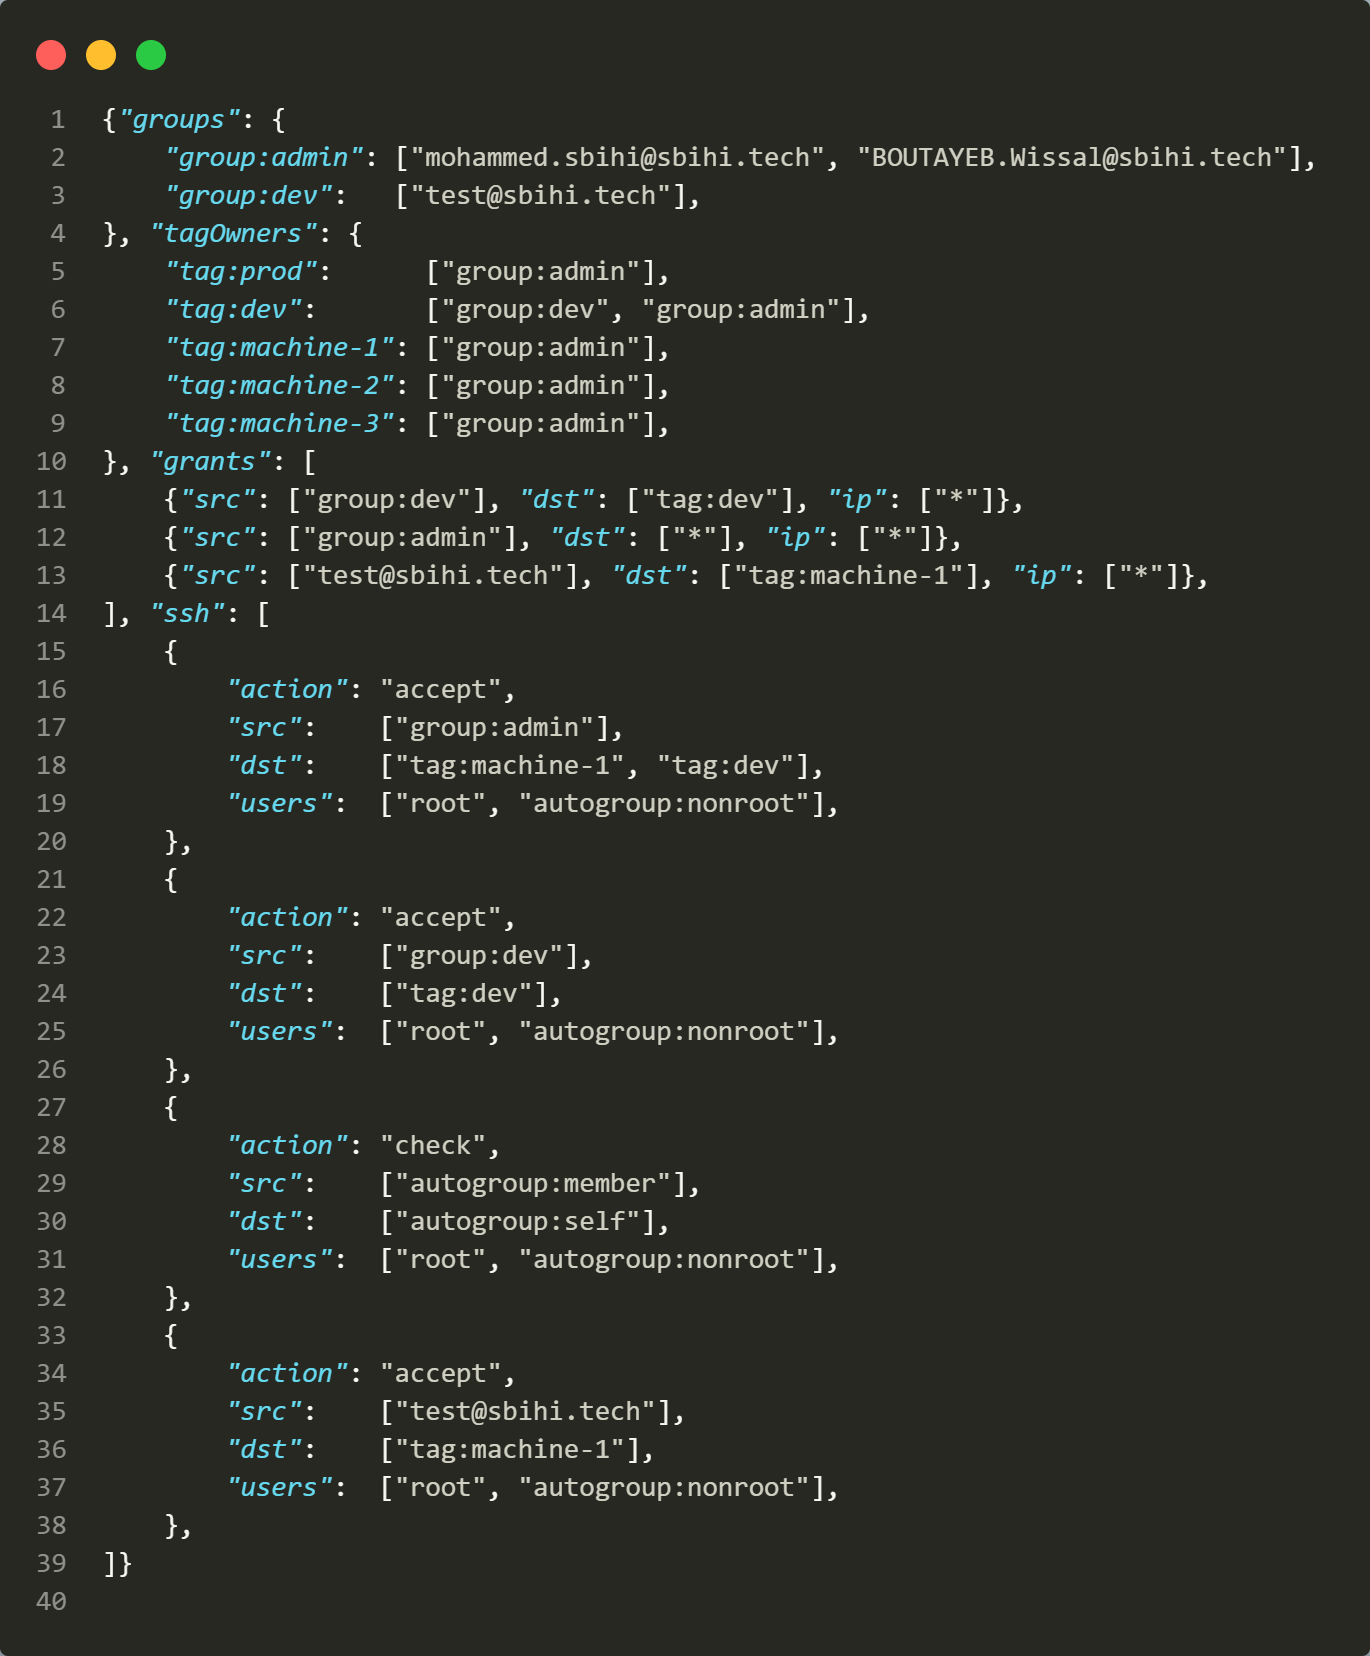
\includegraphics[width=0.95\textwidth]{images/acl-after-acces-granted.png}
	\caption{Etat ACL apres approbation: regle d'acces temporaire ajoutee pour permettre la connexion.}
	\label{fig:acl-after-grant}
\end{figure}
Apres approbation, l'ajout de la regle ACL prouve la transition controlee de l'etat refuse vers l'etat autorise. Le changement n'est pas permanent: il est lie a une demande, une justification et une fenetre temporelle limitee.

\begin{figure}[H]
	\centering
	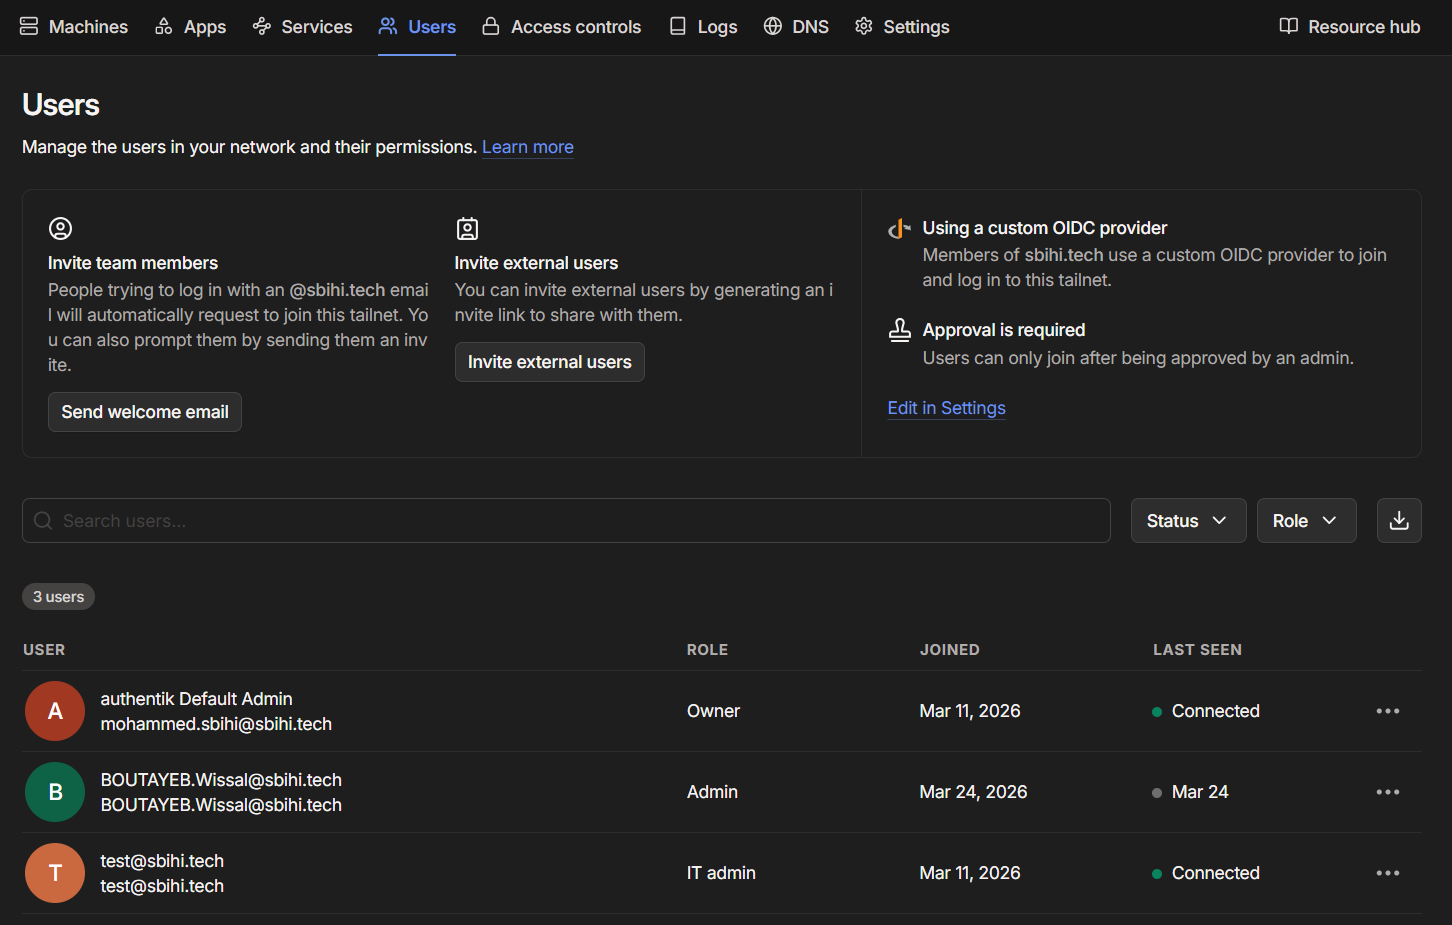
\includegraphics[width=0.9\textwidth]{images/list_of_users_in_tailscale.png}
	\caption{Vue des utilisateurs Tailscale, utilisee pour verifier les identites effectives dans le tailnet.}
	\label{fig:tailscale-users-list}
\end{figure}
La liste des utilisateurs dans le tailnet sert de point de controle supplementaire pour verifier la coherence entre identites IAM et identites reseau. Cette coherence est indispensable pour appliquer des ACL precises et non ambiguës.

\section{Application Flask et base PostgreSQL}
L'application web implemente le cycle de vie des demandes d'acces privilegie.

Les statuts metier principaux sont:
\begin{itemize}
	\item \texttt{pending}: demande en attente d'approbation;
	\item \texttt{approved}: demande acceptee avec expiration;
	\item \texttt{denied}: demande refusee;
	\item \texttt{expired}: acces arrive a echeance.
\end{itemize}

Les regles metier importantes sont:
\begin{itemize}
	\item blocage des doublons \texttt{pending} pour une meme cible/utilisateur;
	\item affichage de l'etat courant et du temps restant pour les acces actifs;
	\item separation des interfaces \textit{user side} et \textit{admin side}.
\end{itemize}

Les ecrans suivants montrent la separation des responsabilites entre utilisateur et administrateur.

\begin{figure}[H]
	\centering
	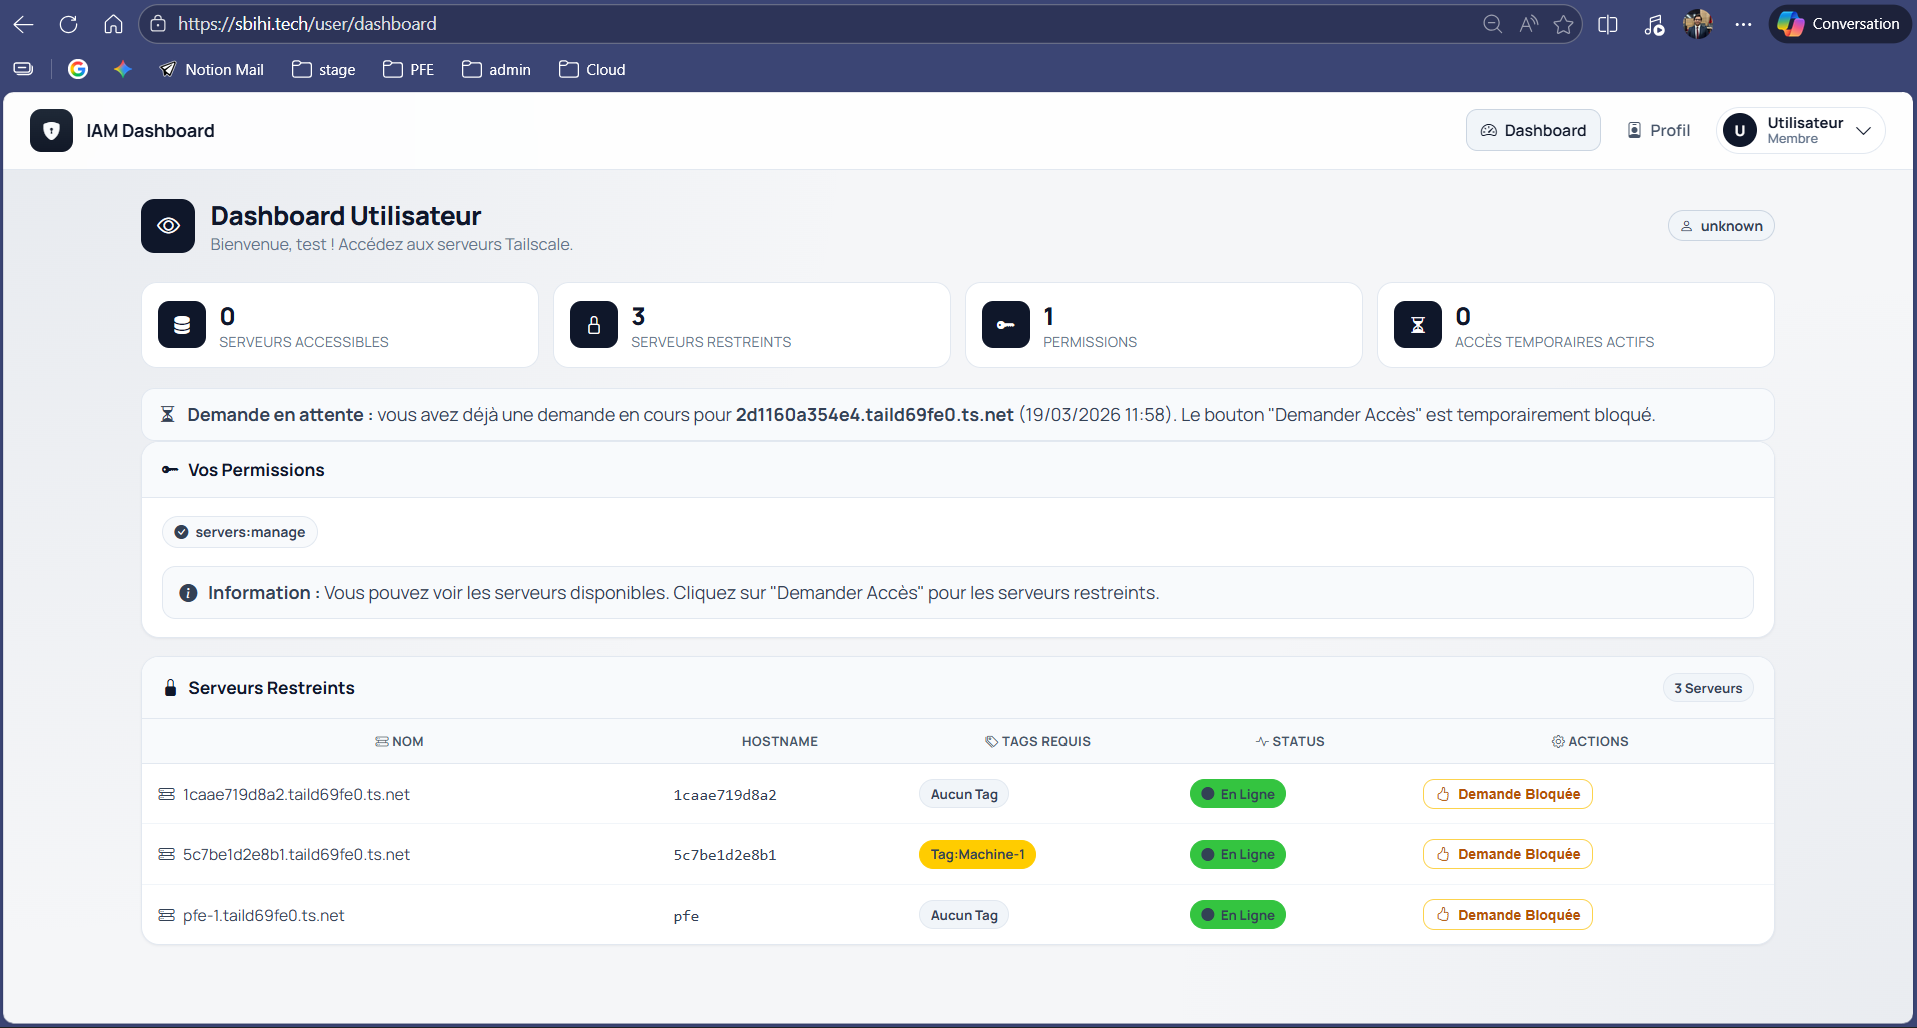
\includegraphics[width=0.95\textwidth]{images/iam_test_dashbord.png}
	\caption{Dashboard utilisateur (user side): consultation de l'etat des acces et lancement d'une demande JIT.}
	\label{fig:user-dashboard}
\end{figure}
Le tableau de bord utilisateur expose uniquement les operations necessaires au role demandeur. Cette limitation de surface fonctionnelle reduit les risques d'erreur et respecte le principe de moindre privilege au niveau applicatif.

\begin{figure}[H]
	\centering
	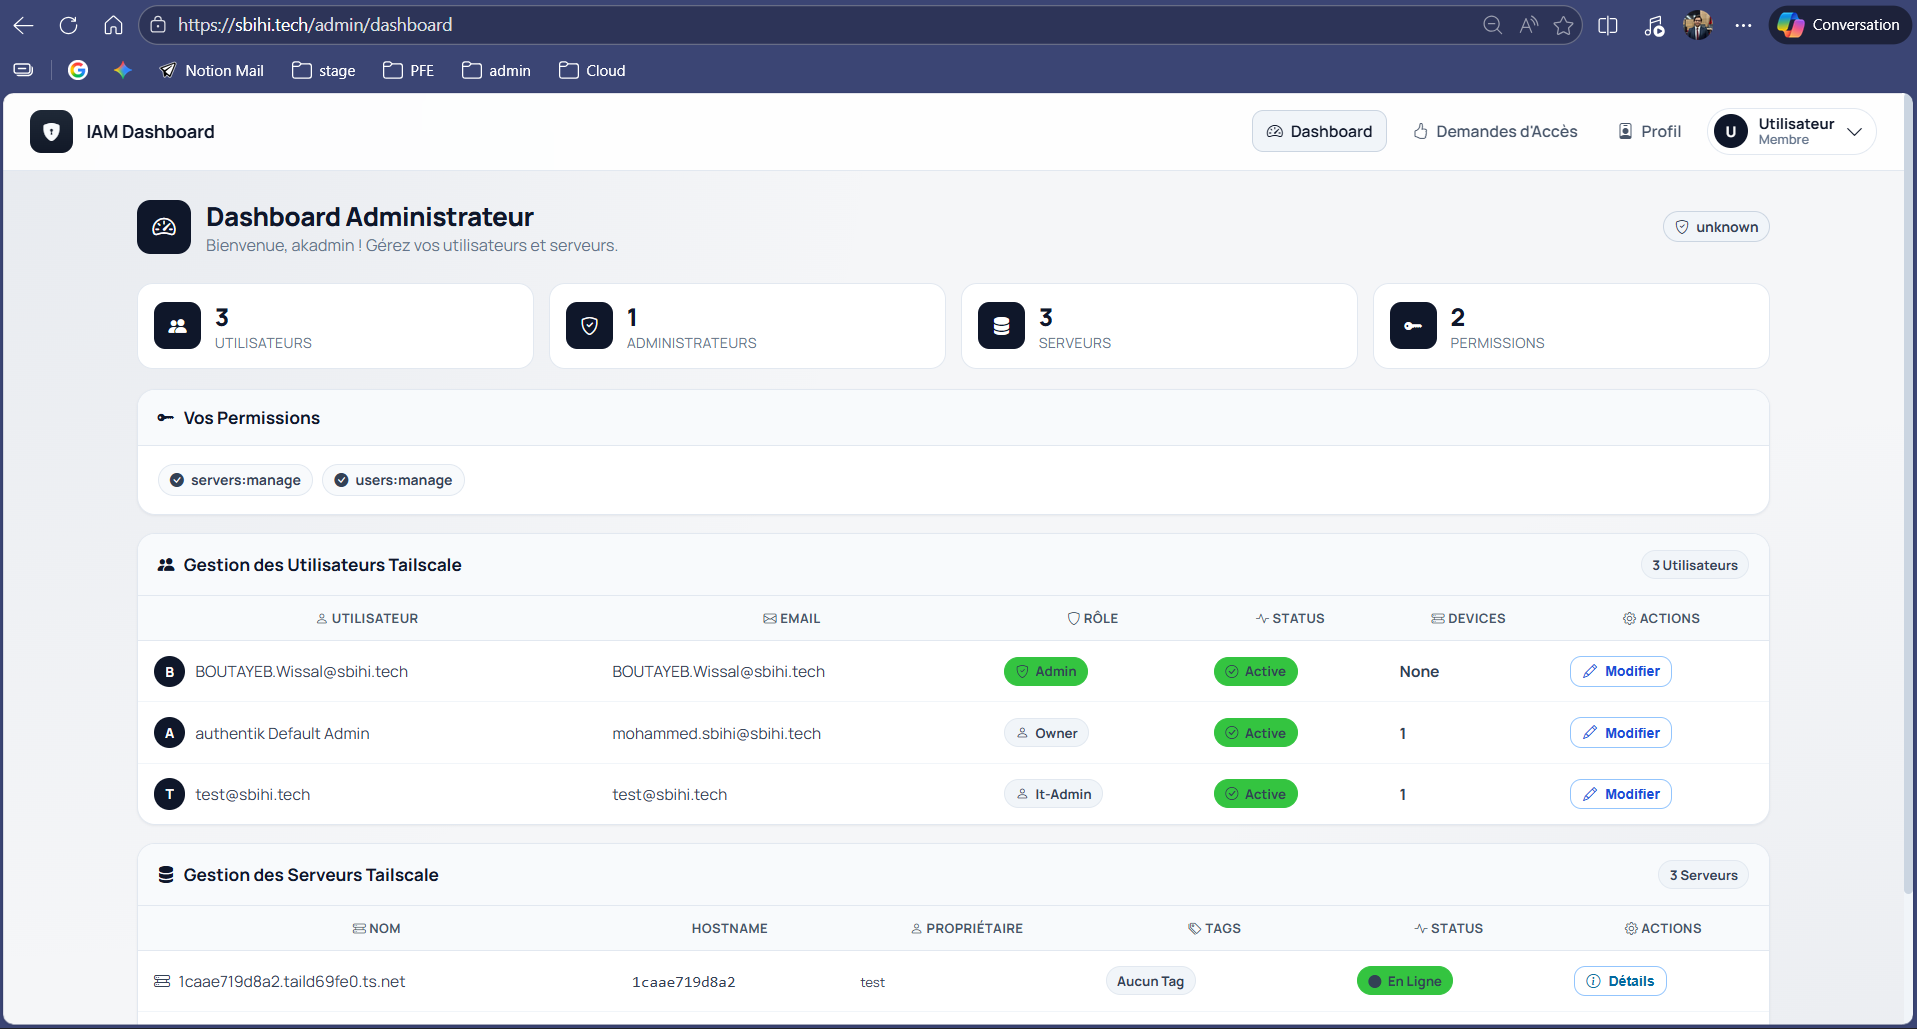
\includegraphics[width=0.95\textwidth]{images/iam_admin_dashbord.png}
	\caption{Dashboard administrateur (admin side): supervision globale des demandes et des actions de gouvernance.}
	\label{fig:admin-dashboard}
\end{figure}
Le tableau de bord administrateur centralise les decisions de gouvernance: validation, refus et suivi des demandes. Il constitue le point de pilotage des privileges temporaires accordes sur l'infrastructure.

\begin{figure}[H]
	\centering
	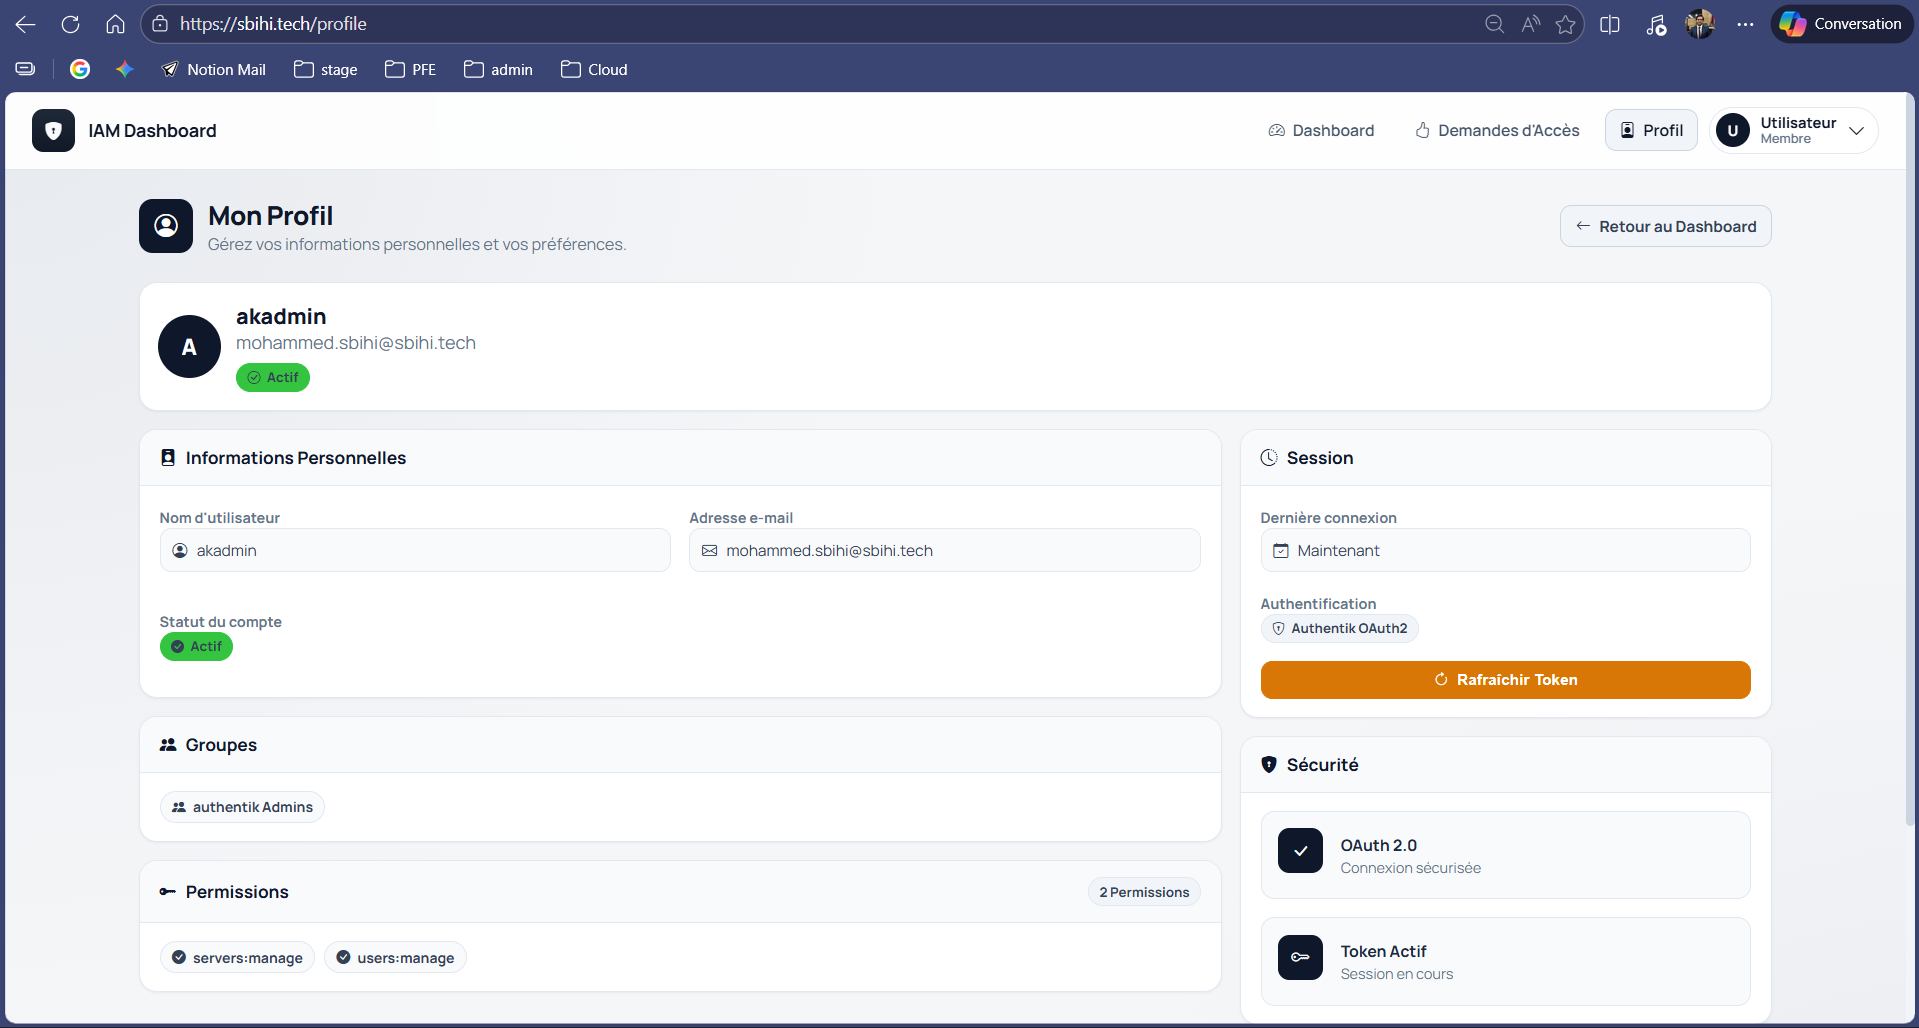
\includegraphics[width=0.95\textwidth]{images/iam_admin_dashbord_profile.png}
	\caption{Vue profil admin: verification des attributs d'identite et des permissions associees au role administrateur.}
	\label{fig:admin-profile}
\end{figure}
La vue profil admin permet de verifier les attributs d'identite utiles a l'audit: roles, groupe et informations de compte. Elle est utile pour confirmer que l'approbation est realisee par un acteur habilite.

\begin{figure}[H]
	\centering
	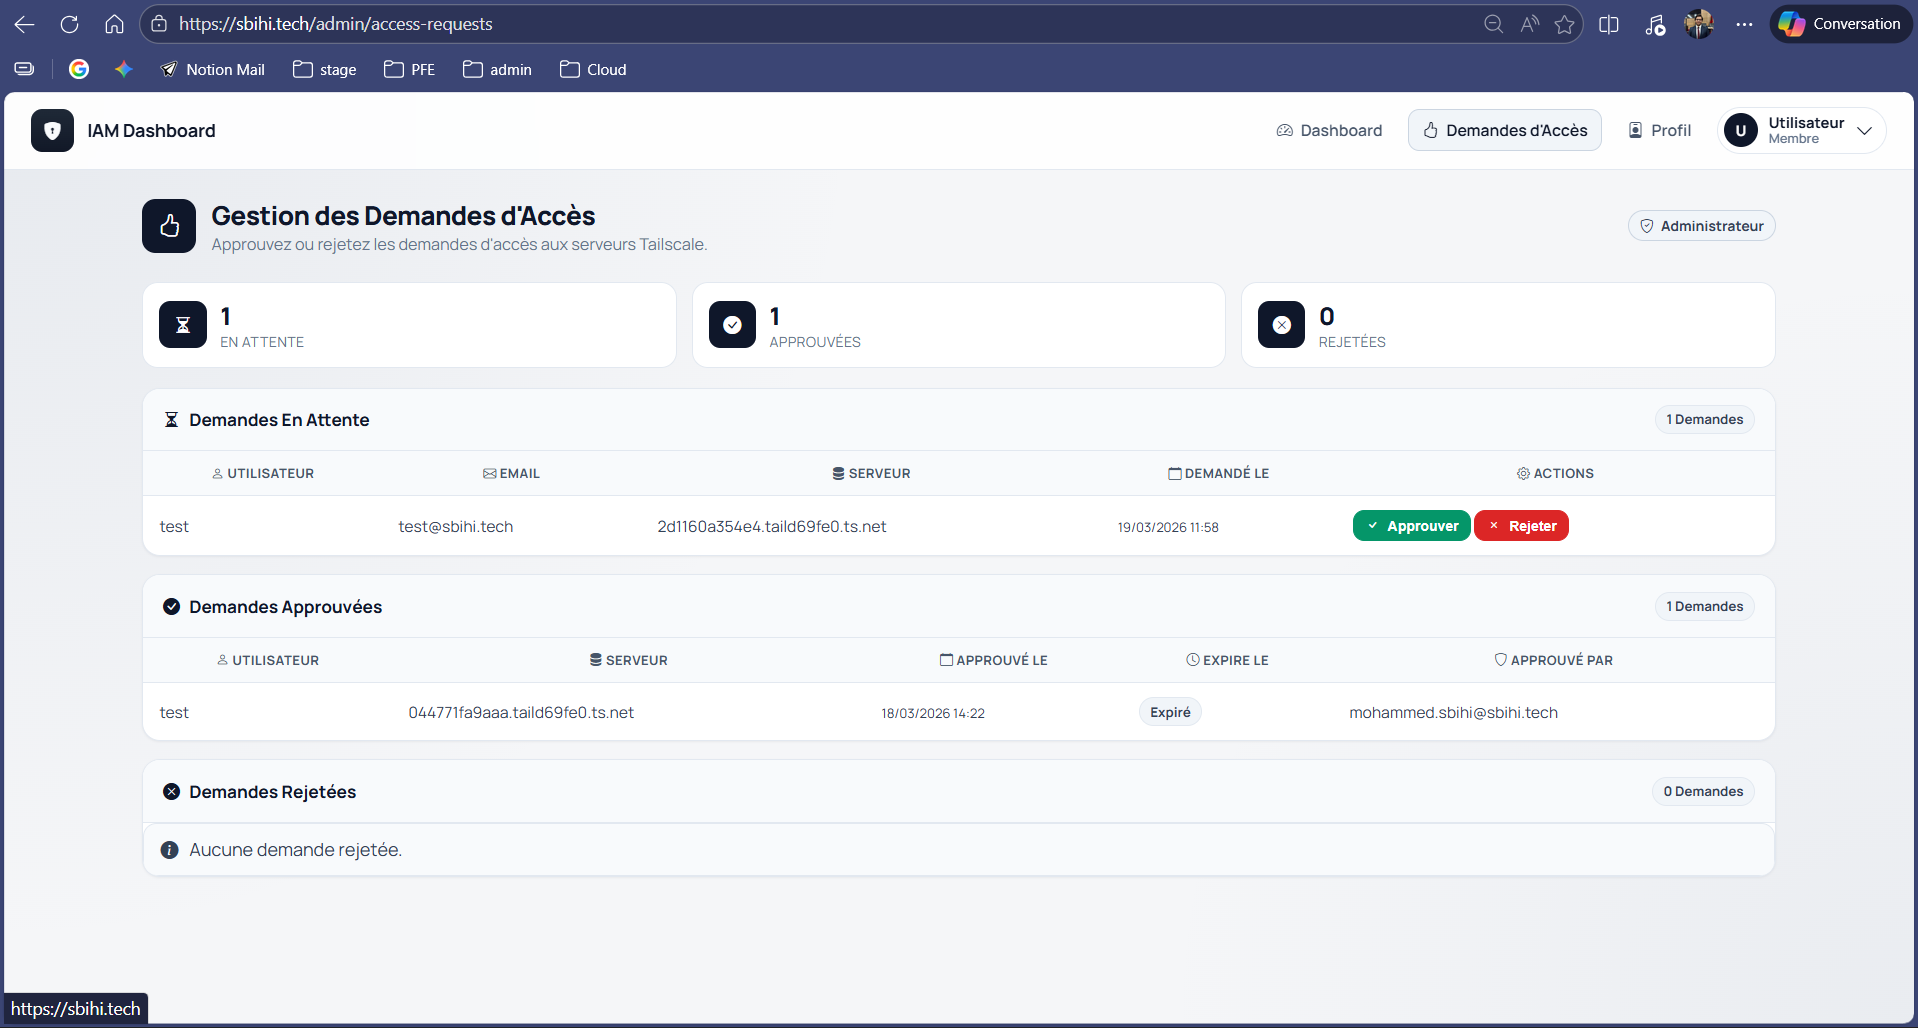
\includegraphics[width=0.95\textwidth]{images/iam_admin_dashbord_acces_request_admin.png}
	\caption{Interface de traitement des demandes d'acces cote admin (liste des requetes et statut).}
	\label{fig:admin-requests-list}
\end{figure}
La file des demandes fournit une vue operationnelle sur les etats \texttt{pending}, \texttt{approved} et \texttt{denied}. Cette visibilite facilite la priorisation des actions et le respect des delais de traitement.

\begin{figure}[H]
	\centering
	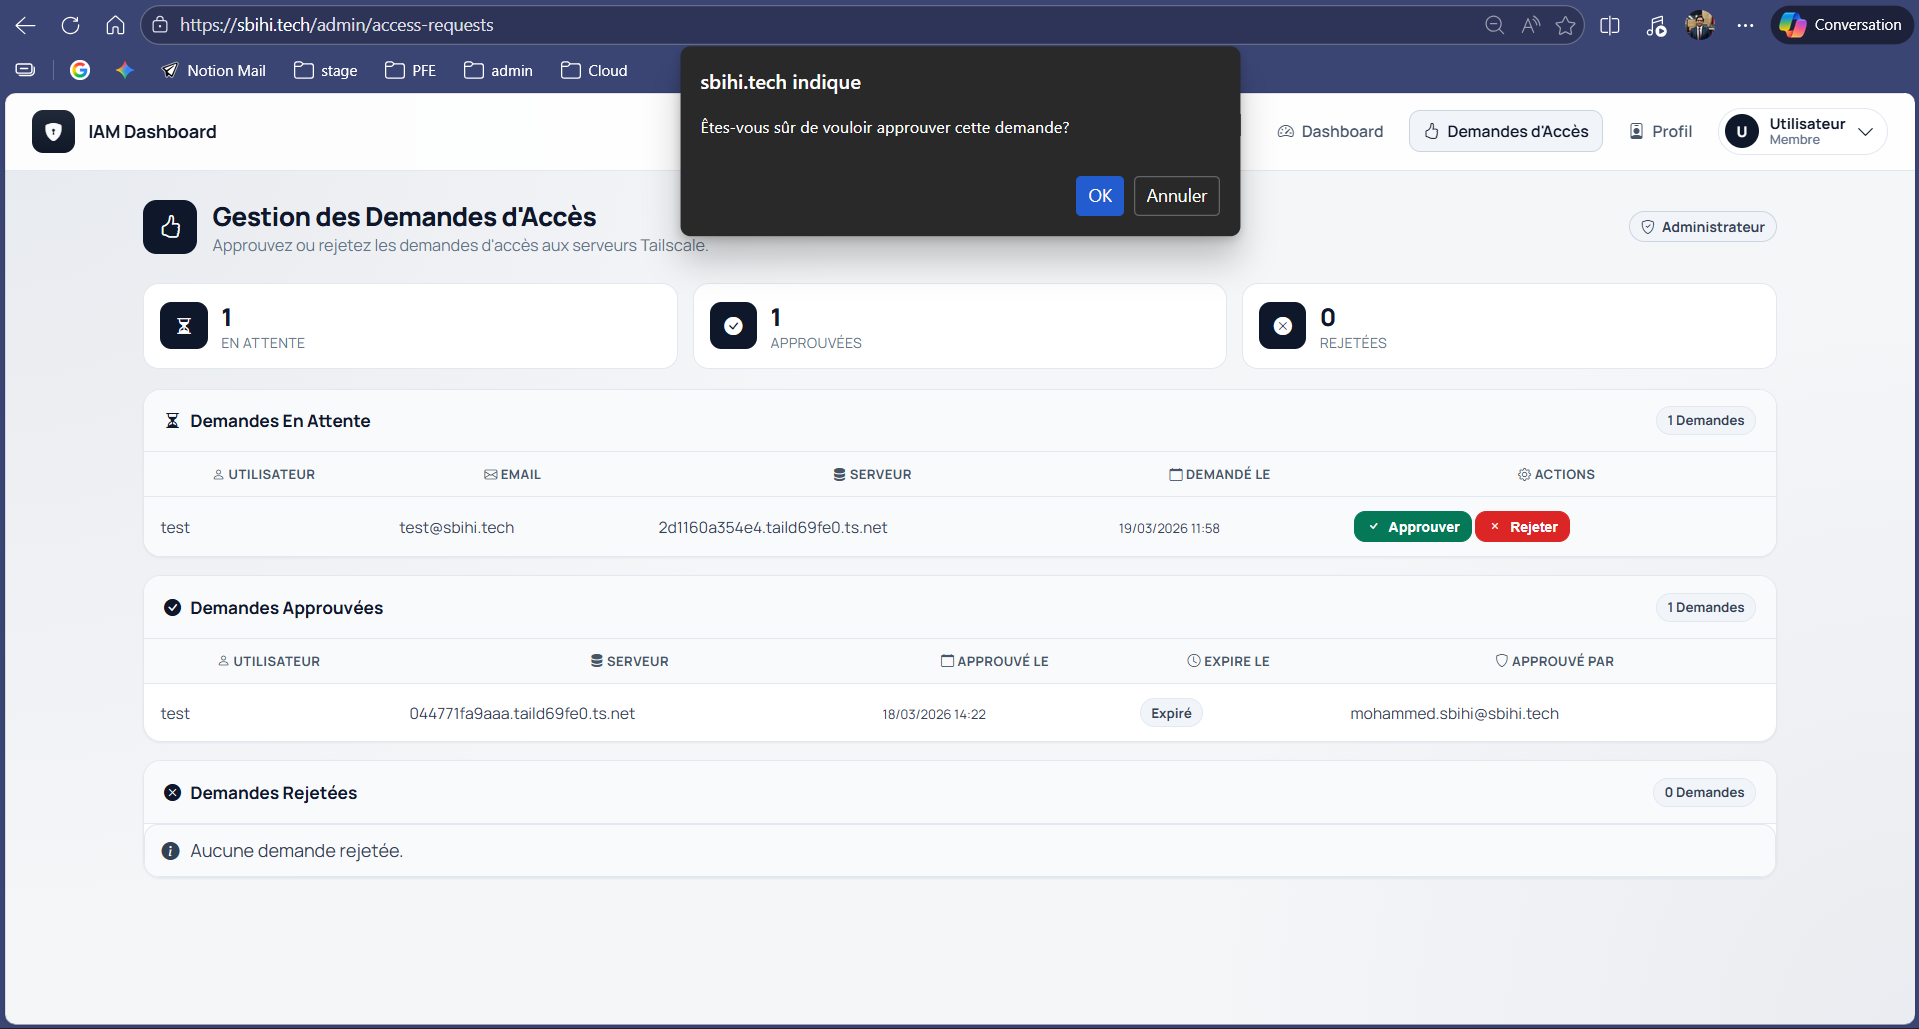
\includegraphics[width=0.95\textwidth]{images/approuve_request_by_admin.png}
	\caption{Action d'approbation d'une demande par l'administrateur, declenchant l'activation ACL temporaire.}
	\label{fig:admin-approve-action}
\end{figure}
Cette preuve met en evidence le point de bascule du workflow JIT. L'approbation ne donne pas un droit global: elle genere un droit cible, borne dans le temps, et directement traçable.

\begin{figure}[H]
	\centering
	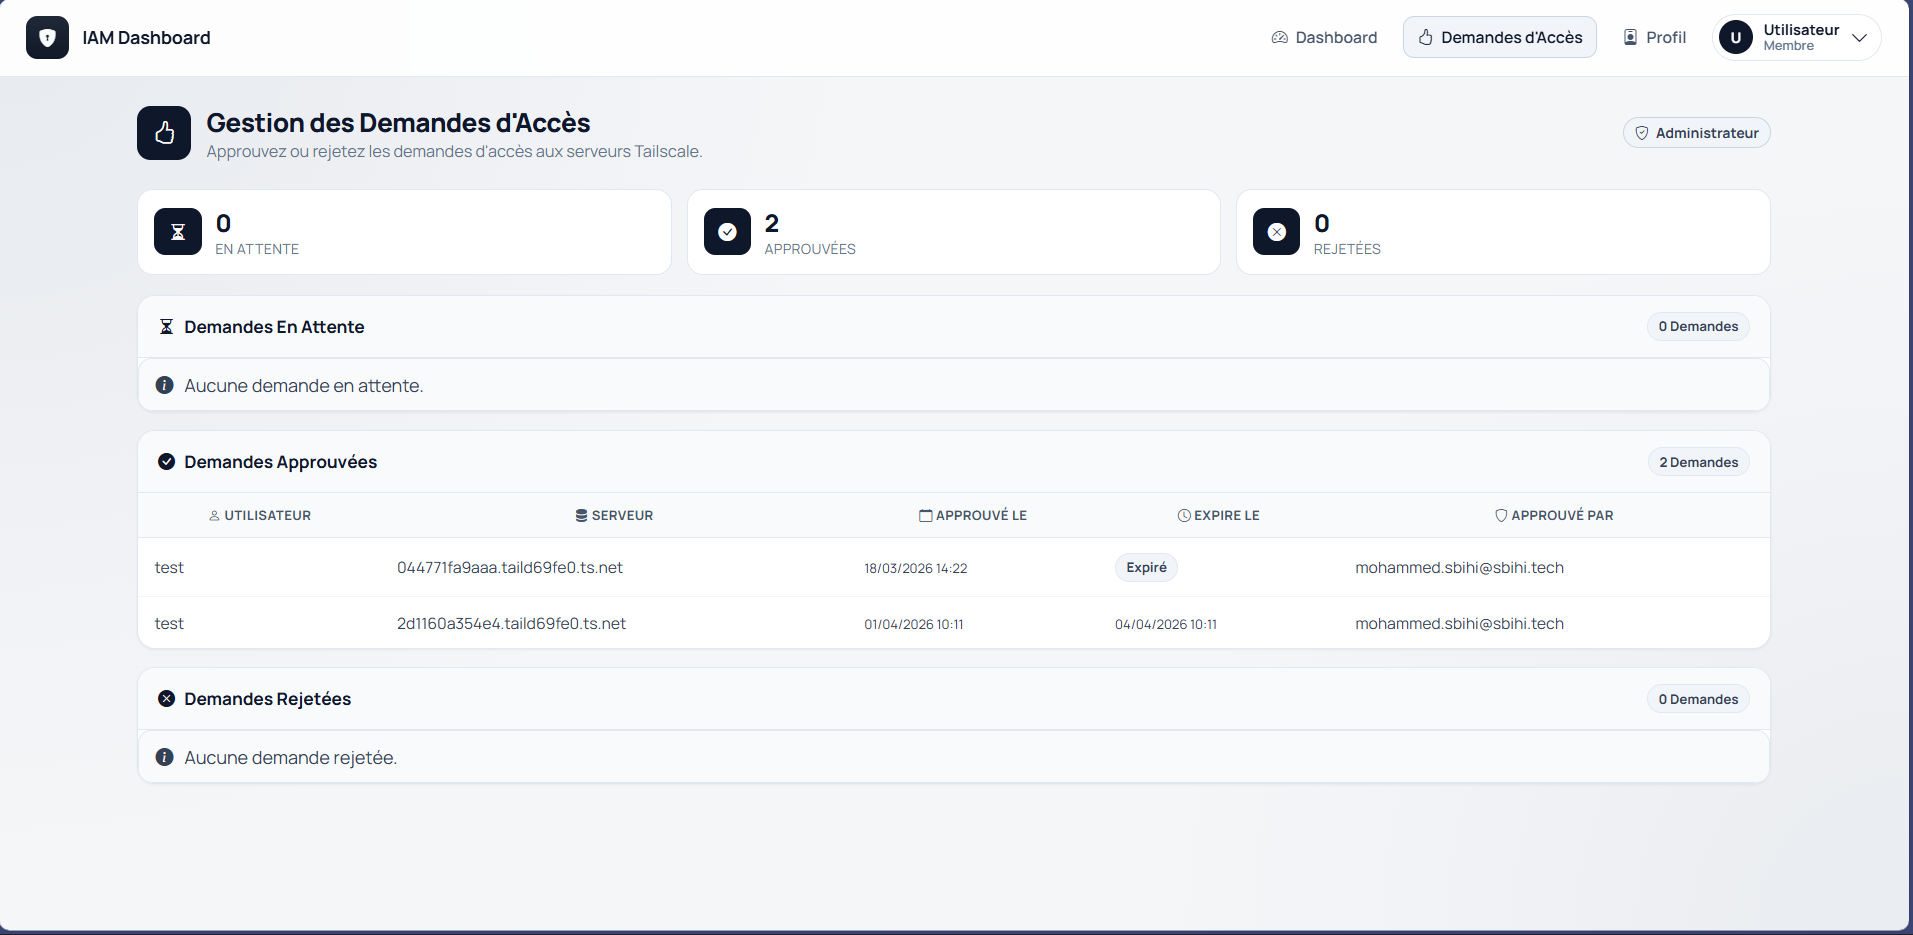
\includegraphics[width=0.95\textwidth]{images/apres_approbation_by_admin_from_admin_side.png}
	\caption{Etat de la demande apres approbation vu depuis l'interface administrateur.}
	\label{fig:admin-after-approval}
\end{figure}
L'etat post-approbation confirme la coherence entre action admin et resultat systeme. La demande est historisee avec son nouveau statut, ce qui simplifie les verifications ulterieures en audit interne.

\begin{figure}[H]
	\centering
	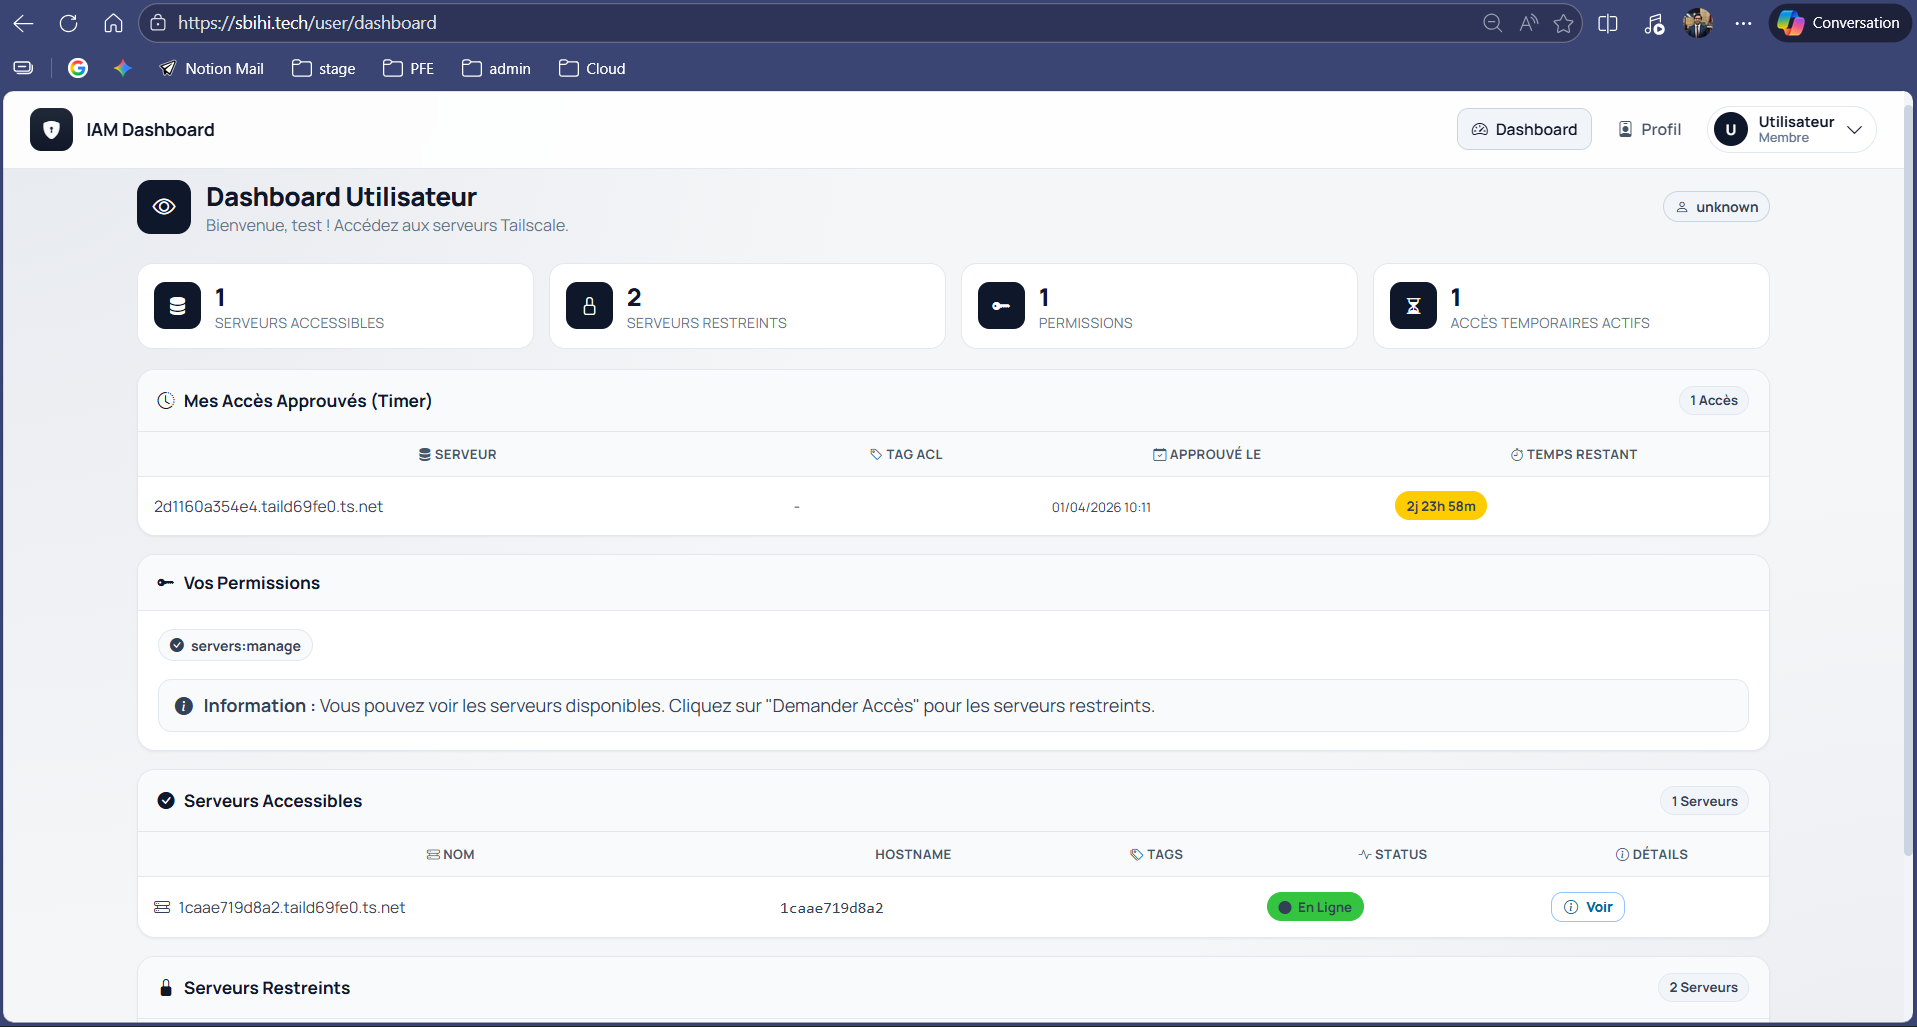
\includegraphics[width=0.95\textwidth]{images/acces_approuver_coter_user.png}
	\caption{Etat cote utilisateur apres validation admin: acces marque comme approuve avec fenetre temporelle active.}
	\label{fig:user-after-approval}
\end{figure}
Le retour cote utilisateur est un element important de gouvernance: il confirme l'etat de la demande et rend visible la temporalite de l'acces, ce qui reduit les ambiguïtés operationnelles.

\section{Moteur JIT Python (ACL\_work)}
Le moteur JIT est implemente dans les scripts Python du dossier \texttt{ACL\_work}.

Fonctions principales:
\begin{itemize}
	\item \texttt{approve\_access\_request(...)}: activation de la regle ACL et mise a jour de la base;
	\item \texttt{revoke\_access\_request(...)}: suppression de la regle ACL et mise a jour de statut;
	\item \texttt{cleanup\_expired\_requests(...)}: nettoyage periodique des droits expires.
\end{itemize}

Le script de maintenance periodique (cron) garantit qu'aucun acces privilegie ne reste actif au-dela de sa duree autorisee.

\begin{figure}[H]
	\centering
	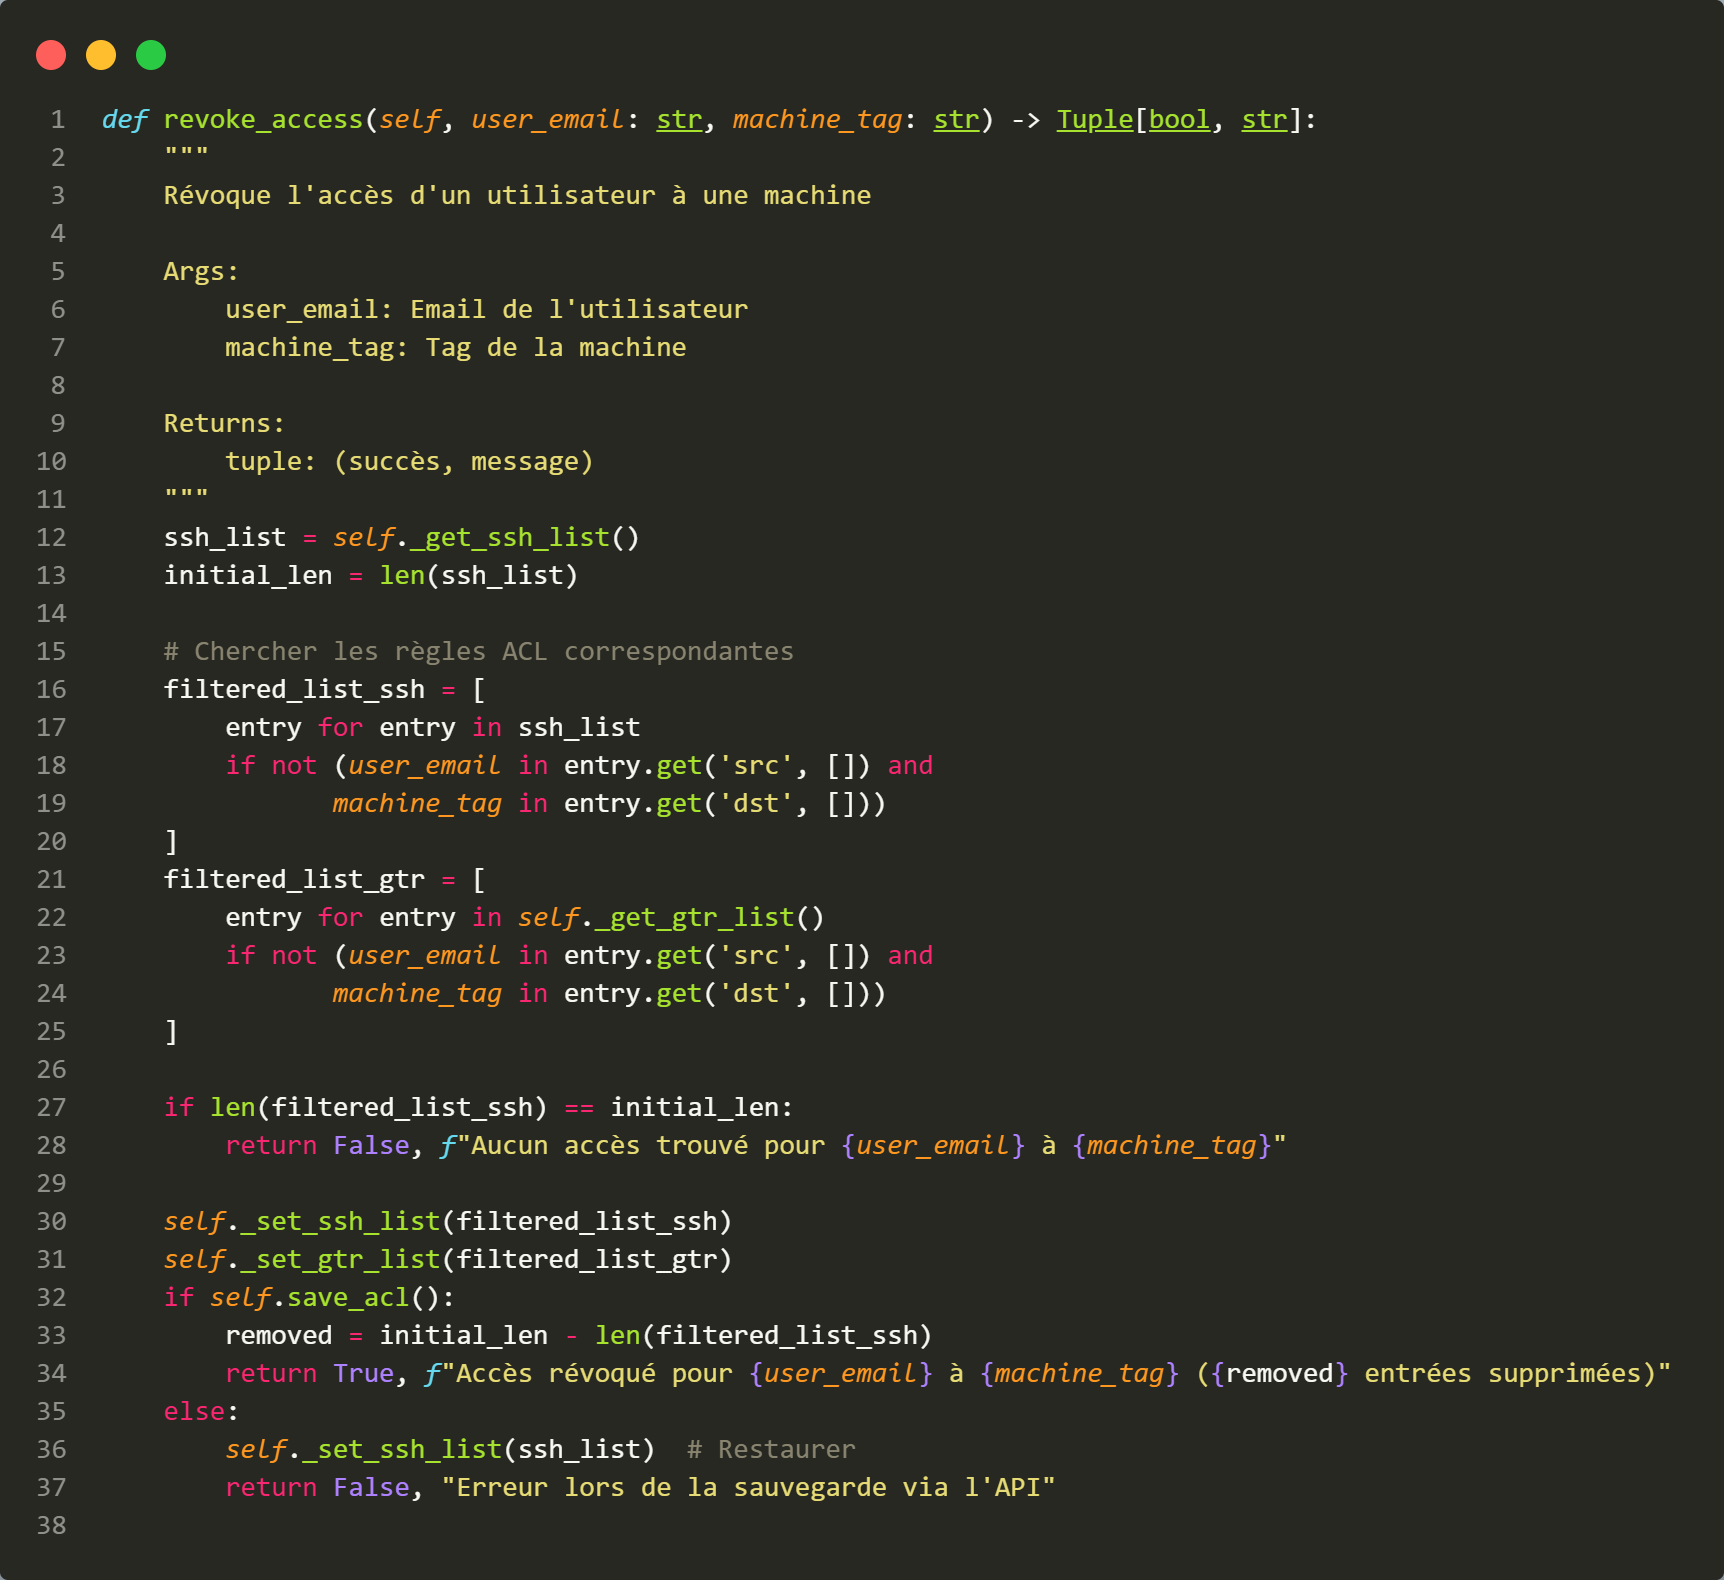
\includegraphics[width=0.95\textwidth]{images/revove_acces_fonction.png}
	\caption{Fonction de revocation d'acces dans le moteur Python: suppression des regles ACL SSH/Grant et gestion du rollback en cas d'echec API.}
	\label{fig:python-revoke-function}
\end{figure}
Le code de revocation montre une logique defensive: suppression ciblee des regles, tentative de sauvegarde via API, puis restauration en cas d'echec. Ce mecanisme limite le risque d'etat incoherent entre base applicative et politique ACL reelle.

\section{Wazuh et observabilite}
Wazuh apporte la visibilite necessaire pour l'audit et la detection d'anomalies.

Les informations attendues dans cette couche sont:
\begin{itemize}
	\item evenements d'authentification et d'echec MFA;
	\item traces d'actions admin (approbation, refus, revocation);
	\item journaux d'acces et d'expiration utiles a la conformite.
\end{itemize}

\subsection{Logging sur les machines cibles}
Sur la machine cible SSH conteneurisee, le journal applicatif de session est force dans \texttt{/var/log/auth.log}. Le script d'entree active \texttt{rsyslog}, cree le fichier de log et injecte un \texttt{PROMPT\_COMMAND} Bash qui journalise chaque commande executee, avec l'identite Tailscale resolue dynamiquement.

\begin{figure}[H]
	\centering
	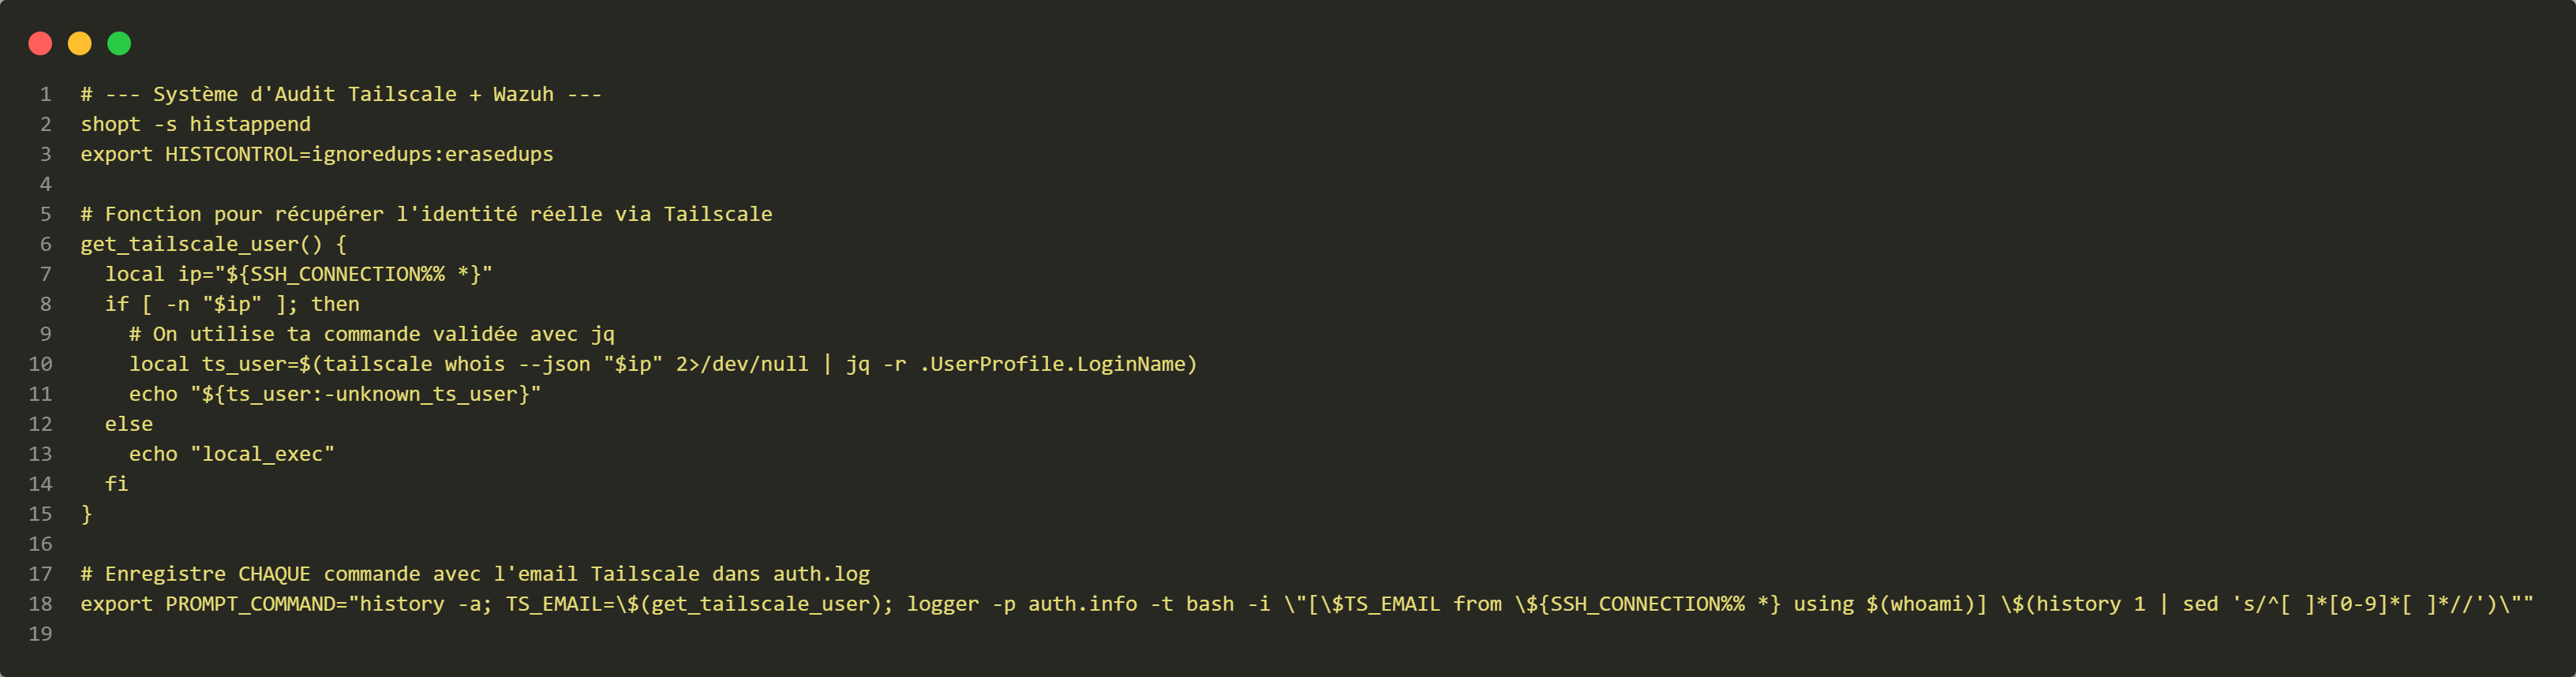
\includegraphics[width=0.96\textwidth]{images/sys_audit.png}
	\caption{Code de journalisation SSH.}
	\label{fig:wazuh-ssh-command-audit}
\end{figure}

Cette approche garantit que les commandes shell sensibles ne restent pas uniquement dans l'historique local utilisateur: elles sont centralisees dans un journal systeme exploitable par l'agent Wazuh.

\subsection{Configuration Wazuh agent et manager}
Le manager Wazuh distribue une configuration agent partagee afin de collecter explicitement \texttt{/var/log/auth.log} avec le format \texttt{syslog}.

\begin{lstlisting}[language=XML, basicstyle=\ttfamily\small]
<agent_config>
  <localfile>
    <log_format>syslog</log_format>
    <location>/var/log/auth.log</location>
  </localfile>
</agent_config>
\end{lstlisting}

Le deploiement Docker du manager monte en plus les decoders, les regles personnalisees et \texttt{agent.conf}, ce qui permet une chaine complete ingestion -> parsing -> alerting sans reconstruire l'image officielle.

\begin{lstlisting}[language=bash, basicstyle=\ttfamily\small]
./decoders/bash_decoder.xml:/var/ossec/etc/decoders/bash_decoder.xml
./rules/bash_rules.xml:/var/ossec/etc/rules/bash_rules.xml
./agents/agent.conf:/var/ossec/etc/shared/default/agent.conf
\end{lstlisting}

\subsection{Decodage et regles d'alerte Bash}
Le decoder \texttt{bash\_audit} extrait les champs utiles (utilisateur Tailscale, source, commande), puis les regles elevent la severite pour les commandes d'administration telles que \texttt{apt}, \texttt{dpkg}, \texttt{rm}, \texttt{nano} et \texttt{vi}.

Ce mecanisme relie directement l'activite shell de la machine cible au SIEM, avec un contexte identite + commande exploitable pour l'audit et la reponse a incident.

\begin{figure}[H]
	\centering
	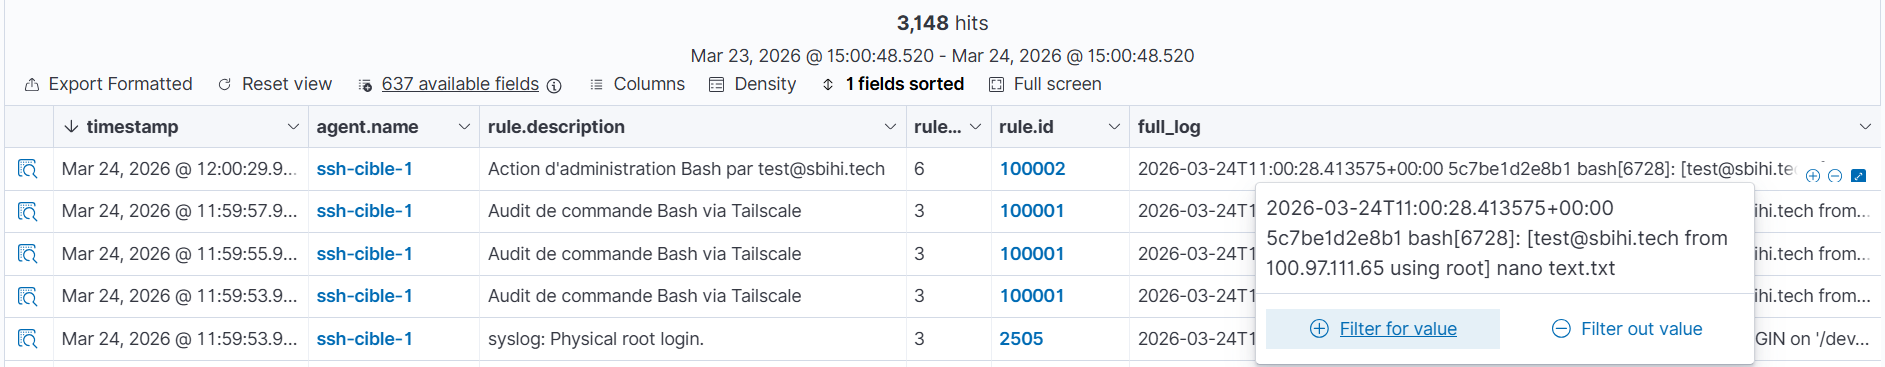
\includegraphics[width=0.96\textwidth]{images/wazuh_log_from ssh showing what the user did in after login to the ssh cible .png}
	\caption{Preuve de centralisation Wazuh: traces de commandes SSH executees sur la machine cible avec contexte utilisateur.}
	\label{fig:wazuh-ssh-command-audit}
\end{figure}
La capture montre la finalite du pipeline: ce qui est tape sur la machine cible est visible dans Wazuh, avec un niveau de detail suffisant pour la tracabilite de conformite et l'investigation technique.

\section{Conclusion du chapitre}
L'implementation par composant confirme la faisabilite technique de la chaine Zero Trust: identite forte, activation conditionnelle des droits, limitation temporelle et tracabilite. Le chapitre suivant valide ces mecanismes par des scenarios de test structures.

\chapterpage{Chapitre 6 : Validation et tests}
\chapter{Scenarios de test et validation}

\section{Introduction du chapitre}
Ce chapitre formalise la strategie de verification adoptee pour demontrer le comportement securitaire de la solution. Il relie chaque test a une propriete Zero Trust attendue et identifie les preuves a collecter pour la validation.

\section{Strategie de test}
La validation repose sur des tests orientes preuve, executes de bout en bout sur les parcours critiques de securite.

Trois familles de tests sont retenues:
\begin{itemize}
	\item \textbf{Tests fonctionnels}: verification du cycle de vie des demandes (creation, approbation, expiration).
	\item \textbf{Tests de securite}: verification du refus par defaut et de l'acces temporaire strictement controle.
	\item \textbf{Tests de tracabilite}: verification de la presence des evenements dans les logs et tableaux de bord.
\end{itemize}

Chaque test est documente avec: preconditions, etapes, resultat attendu, resultat observe et preuves (captures/logs).

\section{Contexte d'execution des tests}
Tous les tests ont ete realises sur une machine virtuelle Azure hebergeant l'ensemble de la plateforme en conteneurs Docker. Les services sont segmentes en plusieurs reseaux Docker (proxy, IAM, cible SSH, Wazuh), avec un proxy inverse en frontal pour l'exposition controlee des interfaces web.

Ce contexte est important pour l'interpretation des resultats:
\begin{itemize}
	\item la connectivite reseau inter-service est gouvernee par les reseaux Docker et non par un flat network;
	\item la cible SSH est isolee dans son domaine de communication et n'est accessible qu'apres activation ACL;
	\item la collecte de logs vers Wazuh est verifiee dans le meme environnement de production maquette.
\end{itemize}

\section{Cas de test IAM/PIM/PAM}
\subsection{TC-01: Authentification forte IAM}
\textbf{Preconditions}: utilisateur actif dans Authentik et MFA configure.

\textbf{Etapes}:
\begin{enumerate}
	\item ouvrir la page de connexion de l'application;
	\item saisir identifiant et mot de passe;
	\item valider le second facteur TOTP.
\end{enumerate}

\textbf{Attendu}: acces accorde uniquement apres validation MFA.

\textbf{Preuves}: capture login, capture ecran MFA, event d'authentification.

\begin{figure}[H]
	\centering
	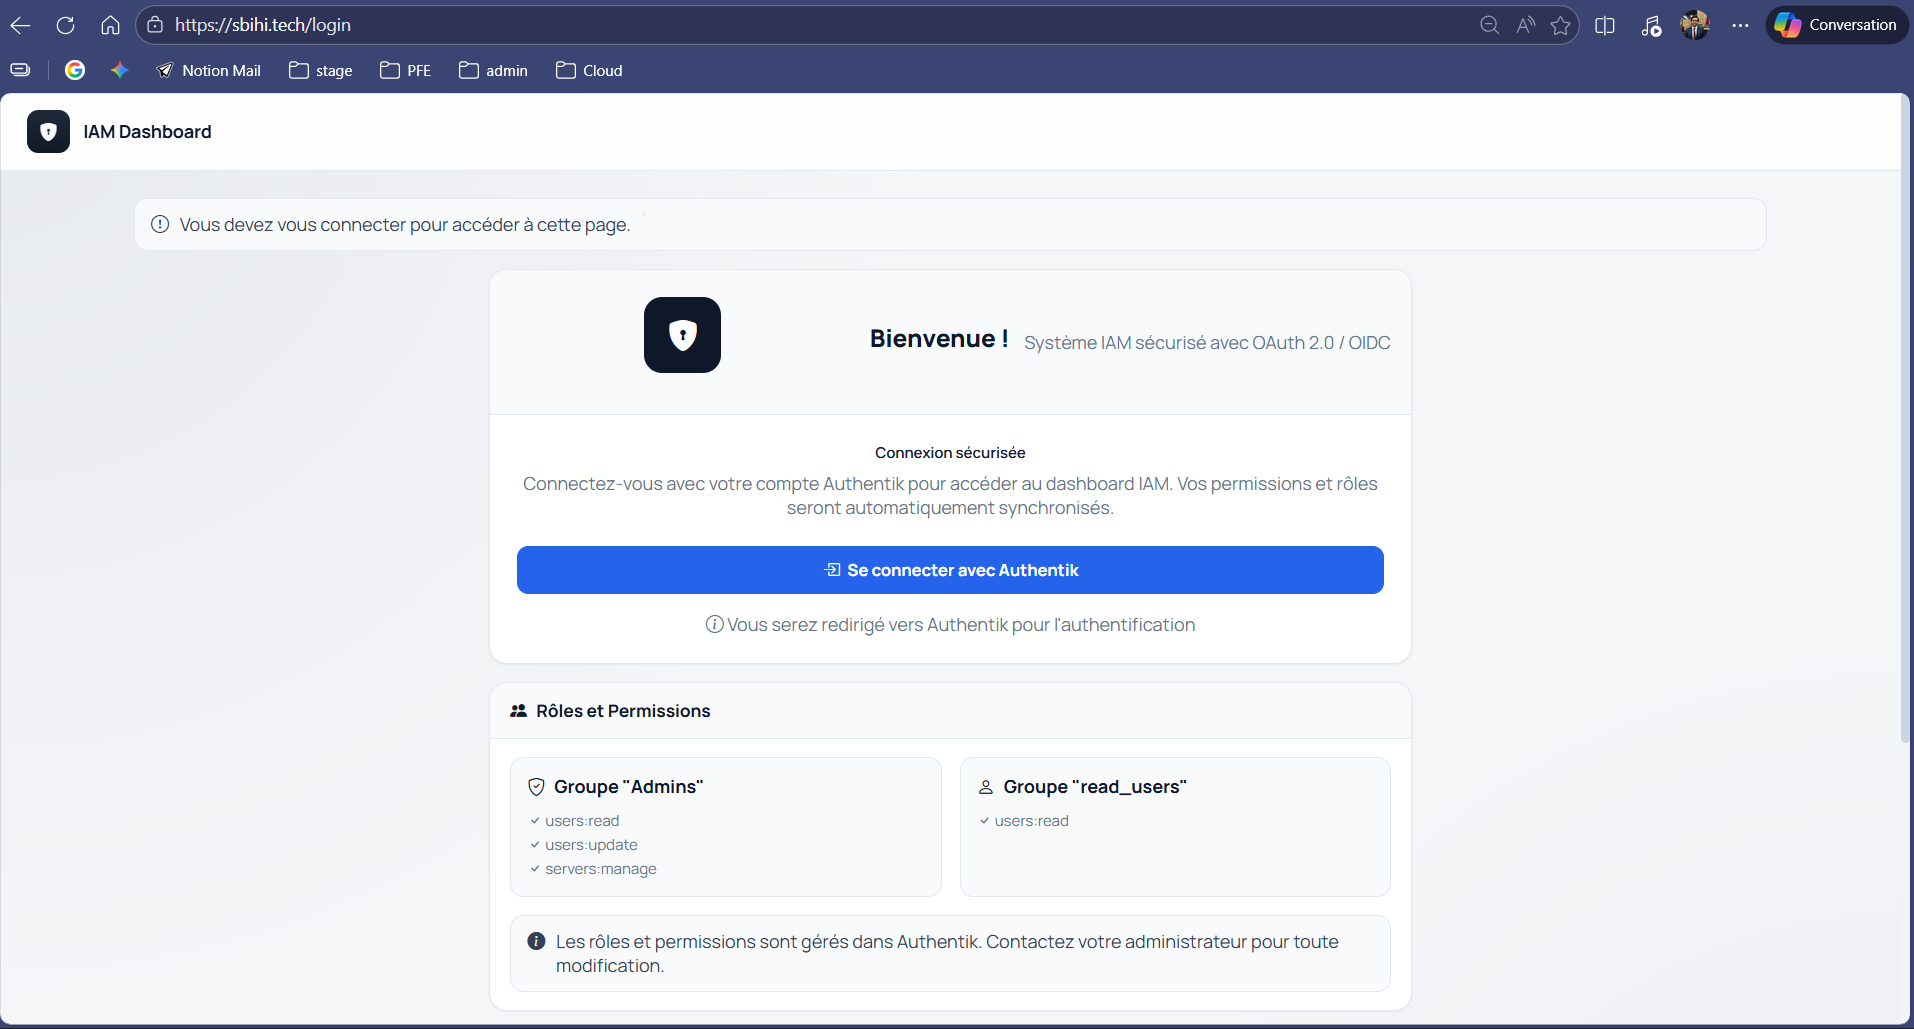
\includegraphics[width=0.9\textwidth]{images/iam_dashbord_login.png}
	\caption{Preuve TC-01: ecran de connexion IAM avant emission d'une session valide.}
	\label{fig:tc01-login}
\end{figure}
Cette image confirme que le point d'entree du systeme passe par la couche IAM. Dans la logique Zero Trust, cette etape est indispensable pour associer toute action ulterieure a une identite authentifiee.

\subsection{TC-02: Creation d'une demande JIT}
\textbf{Preconditions}: utilisateur sans acces privilegie permanent sur la cible.

\textbf{Etapes}:
\begin{enumerate}
	\item se connecter a l'interface utilisateur;
	\item soumettre une demande d'acces a une machine cible;
	\item tenter de soumettre une deuxieme demande identique si la premiere est \texttt{pending}.
\end{enumerate}

\textbf{Attendu}: la premiere demande passe \texttt{pending}; la seconde est bloquee par regle anti-doublon.

\textbf{Preuves}: capture dashboard user, capture message de blocage anti-doublon.

La validation de ce cas repose sur l'existence d'un controle anti-doublon cote application. Ce controle evite les demandes paralleles contradictoires et stabilise la gouvernance des droits temporaires.

\subsection{TC-03: Approbation admin et activation ACL}
\textbf{Preconditions}: demande \texttt{pending} visible cote administration.

\textbf{Etapes}:
\begin{enumerate}
	\item ouvrir le dashboard admin;
	\item approuver la demande;
	\item verifier le statut et la date d'expiration;
	\item verifier la mise a jour de la politique ACL.
\end{enumerate}

\textbf{Attendu}: statut \texttt{approved}, ACL active, fenetre TTL demarree.

\textbf{Preuves}: capture action admin, capture ACL apres approbation, trace applicative.

\begin{figure}[H]
	\centering
	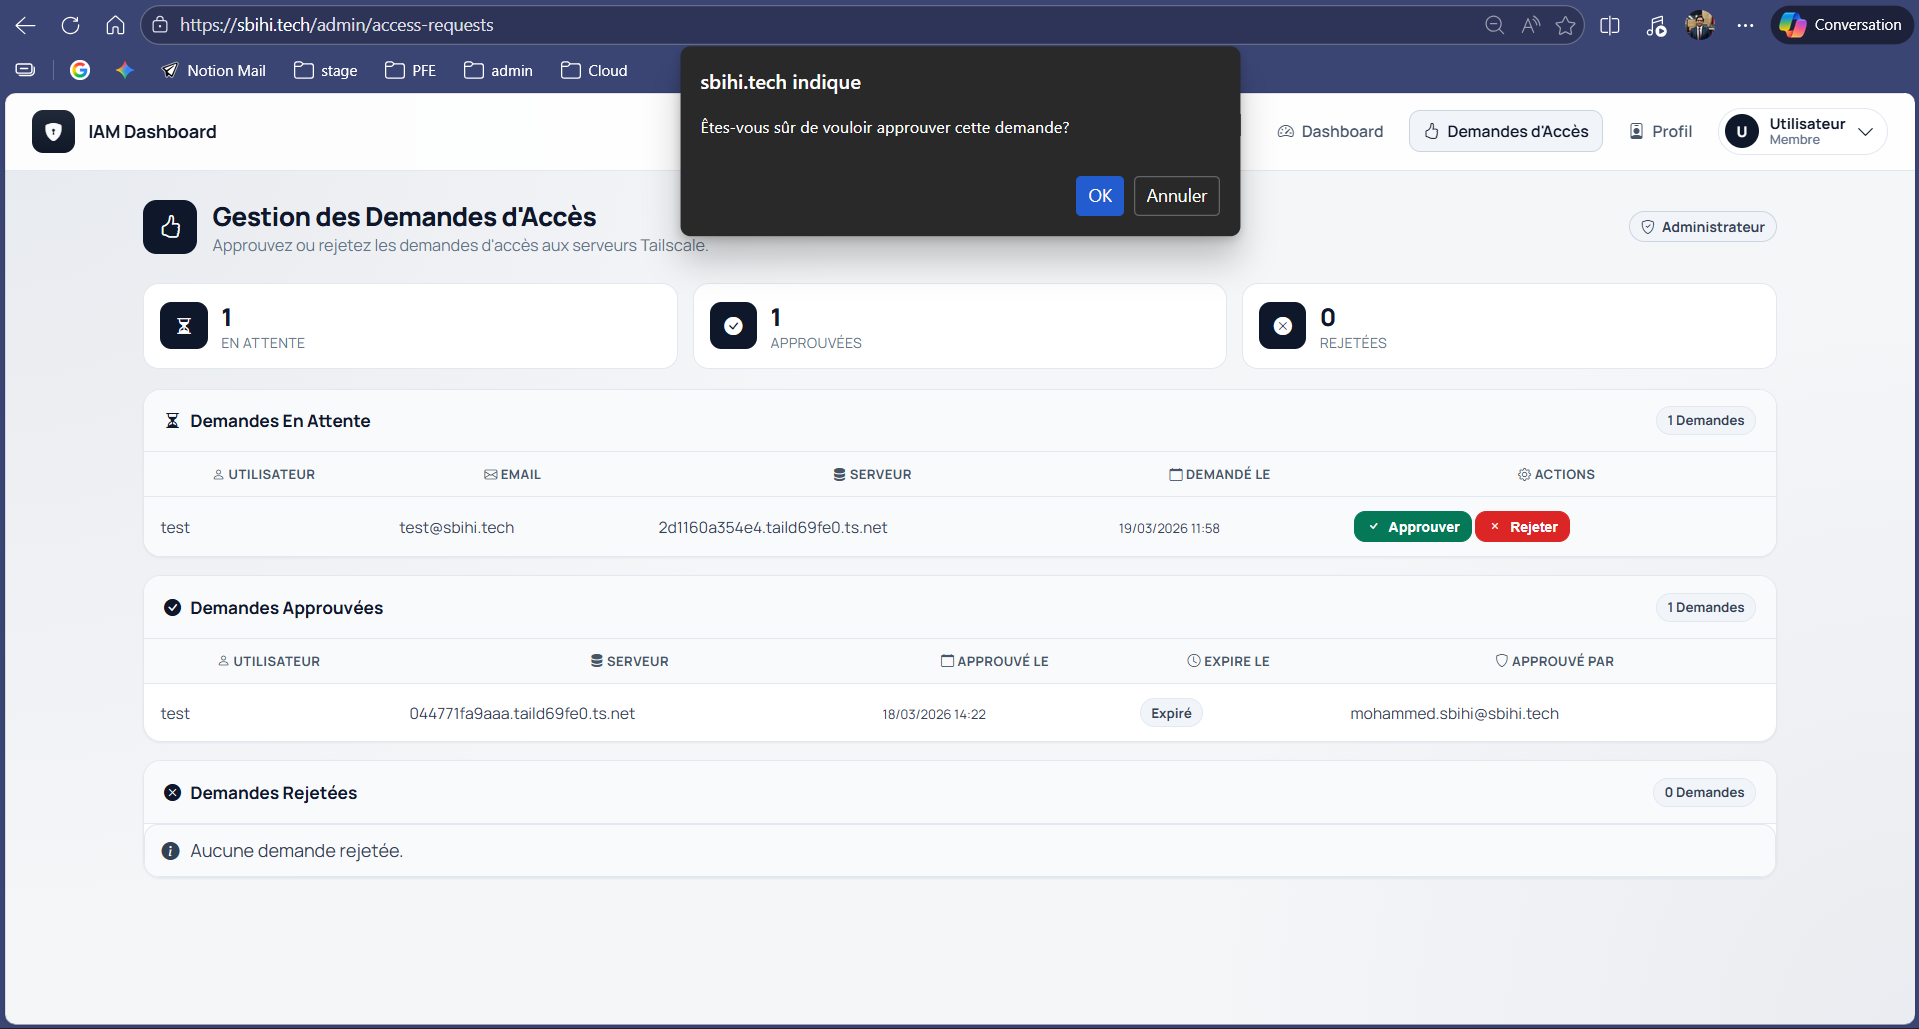
\includegraphics[width=0.95\textwidth]{images/approuve_request_by_admin.png}
	\caption{Preuve TC-03: action d'approbation executee par l'administrateur.}
	\label{fig:tc03-admin-approval}
\end{figure}
La capture montre que l'activation du droit est le resultat d'une decision humaine explicite. Cette etape introduit une validation de gouvernance avant toute modification reseau effective.

\begin{figure}[H]
	\centering
	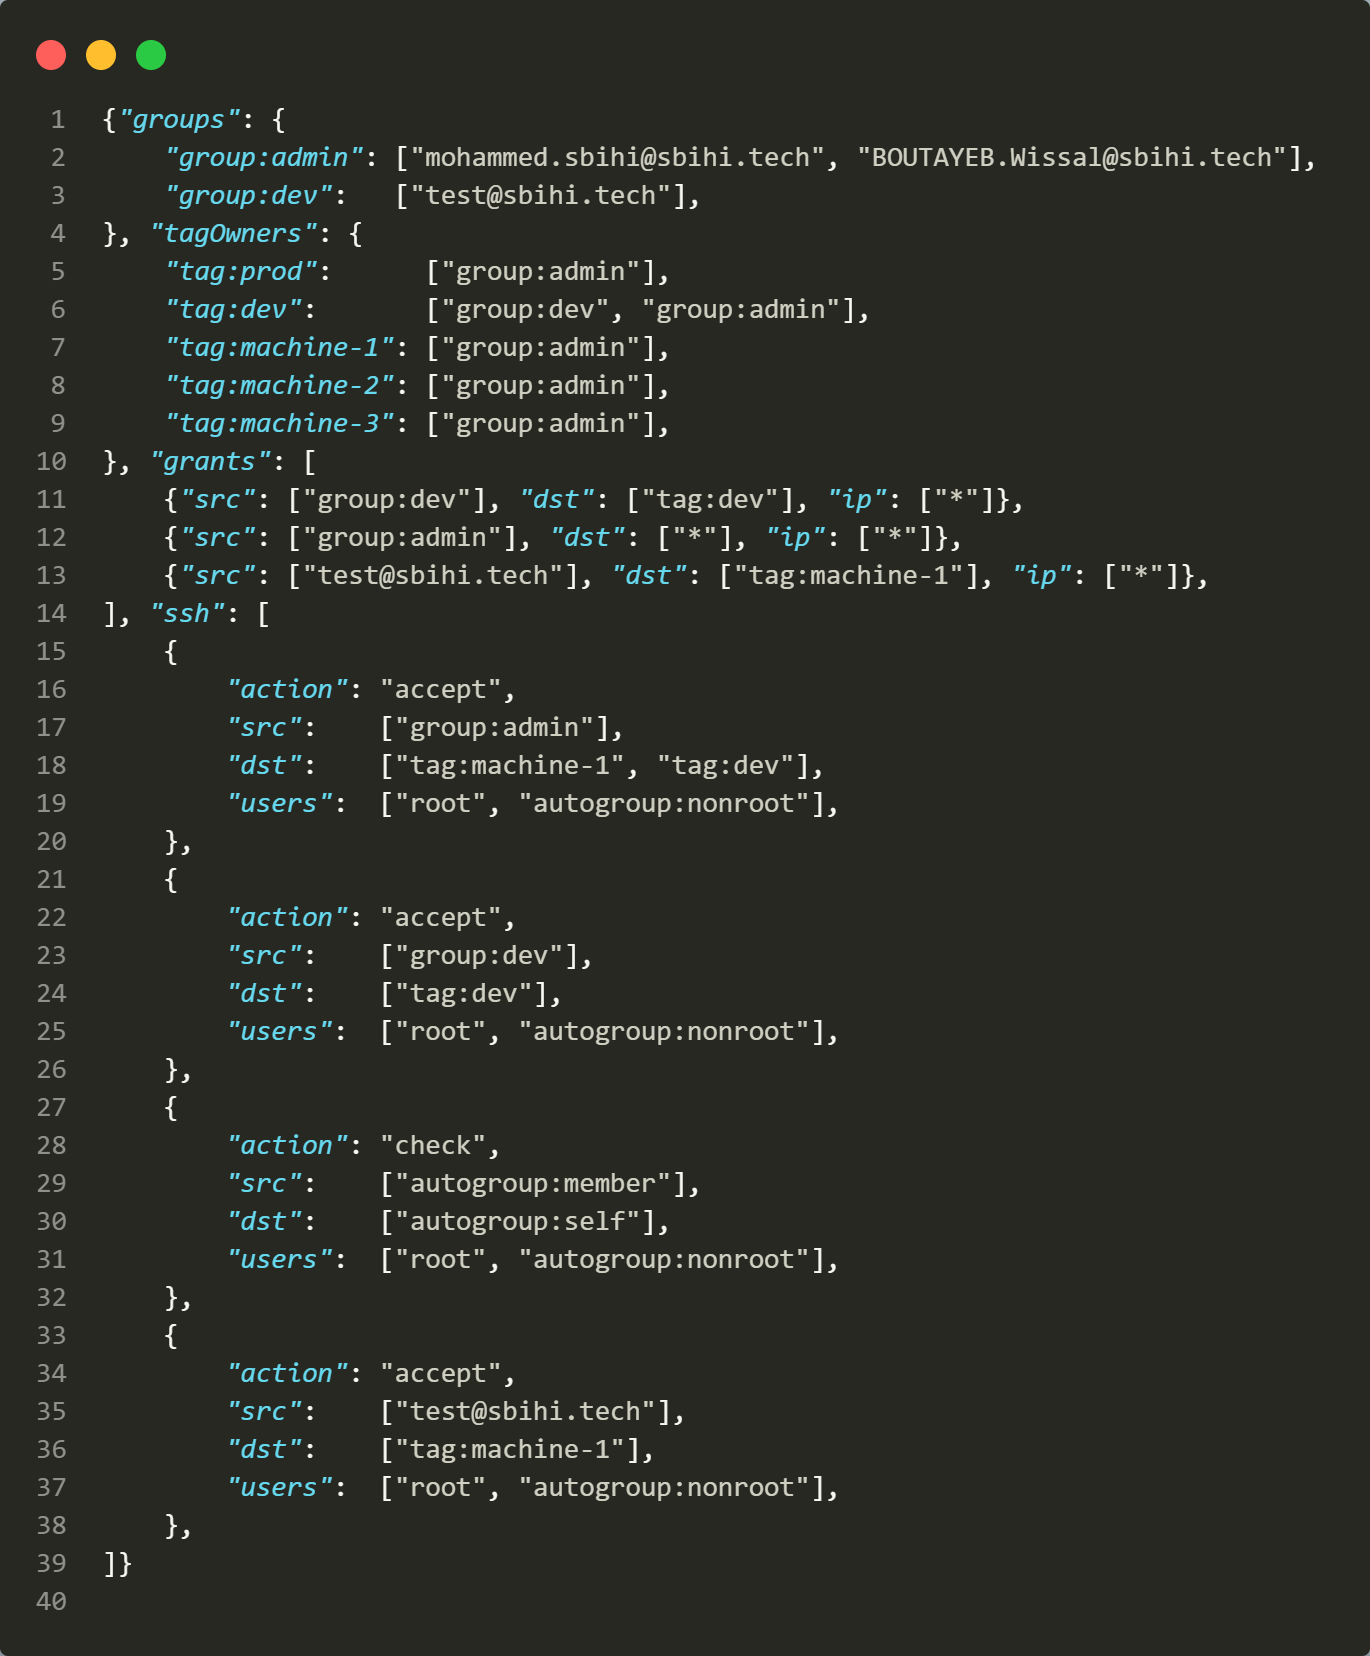
\includegraphics[width=0.95\textwidth]{images/acl-after-acces-granted.png}
	\caption{Preuve TC-03: regle ACL active apres approbation de la demande.}
	\label{fig:tc03-acl-after}
\end{figure}
L'evolution de la politique ACL apres approbation demontre le chainage correct entre workflow applicatif et enforcement reseau. Cette coherence est centrale pour prouver l'efficacite du mecanisme JIT.

\subsection{TC-04: SSH avant et apres approbation}
\textbf{Preconditions}: une cible SSH integree et une demande en cours de traitement.

\textbf{Etapes}:
\begin{enumerate}
	\item tenter une connexion SSH avant approbation;
	\item approuver la demande;
	\item retenter la connexion SSH pendant la fenetre active.
\end{enumerate}

\textbf{Attendu}: echec avant approbation, succes apres approbation.

\textbf{Preuves}: captures terminal avant/apres, logs de connexion.

\begin{figure}[H]
	\centering
	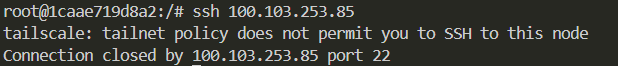
\includegraphics[width=0.98\textwidth]{images/ssh_failed_before_from user test@sbihi.tech to a other machine in the tailscale network.png}
	\caption{Preuve TC-04 (avant approbation): tentative SSH refusee car aucun droit temporaire n'est encore actif.}
	\label{fig:tc04-ssh-failed-before}
\end{figure}
Le refus observe avant approbation valide le comportement attendu en mode \textit{deny by default}. L'infrastructure applique bien l'absence de confiance implicite envers les utilisateurs non autorises.

\begin{figure}[H]
	\centering
	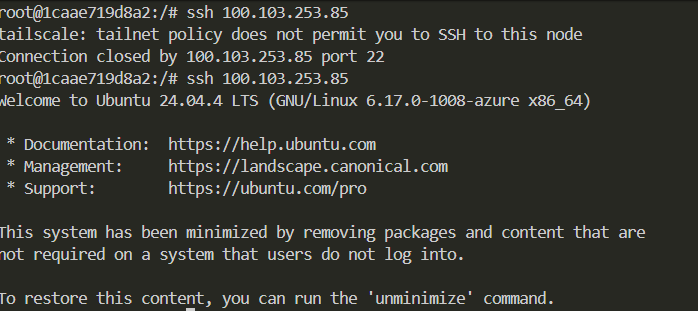
\includegraphics[width=0.98\textwidth]{images/ssh_accepted_before_from user test@sbihi.tech to a other machine in the tailscale network.png}
	\caption{Preuve TC-04 (apres approbation): tentative SSH acceptee pendant la fenetre d'acces JIT.}
	\label{fig:tc04-ssh-success-after}
\end{figure}
Le succes de connexion apres approbation confirme la levée de restriction strictement conditionnee. Ce comportement binaire avant/apres est la preuve la plus lisible de l'efficacite du couple approbation admin + ACL dynamique.

\subsection{TC-05: Expiration automatique et revocation}
\textbf{Preconditions}: acces \texttt{approved} avec TTL court.

\textbf{Etapes}:
\begin{enumerate}
	\item attendre l'expiration ou lancer le script de nettoyage;
	\item verifier le passage au statut \texttt{expired};
	\item retenter une connexion SSH.
\end{enumerate}

\textbf{Attendu}: acces revoque, ACL retiree, connexion SSH refusee.

\textbf{Preuves}: sortie script \texttt{cleanup}, capture SSH refuse, log d'expiration.

Ce cas final est critique, car il valide la non-persistance des privileges. L'absence de nettoyage automatique annulerait le benefice Zero Trust et recreerait un risque d'acces permanent.

\subsection{TC-06: Tracabilite Wazuh des commandes SSH}
\textbf{Preconditions}: connexion SSH active sur la machine cible et agent Wazuh operationnel.

\textbf{Etapes}:
\begin{enumerate}
\item executer des commandes shell sur la cible pendant une fenetre JIT autorisee;
\item verifier l'ecriture des traces dans \texttt{/var/log/auth.log};
\item confirmer la remontee des evenements dans le dashboard Wazuh.
\end{enumerate}

\textbf{Attendu}: les commandes executees apparaissent dans Wazuh avec le contexte utilisateur/source.

\textbf{Preuves}: capture Wazuh de logs SSH centralises.

\begin{figure}[H]
	\centering
	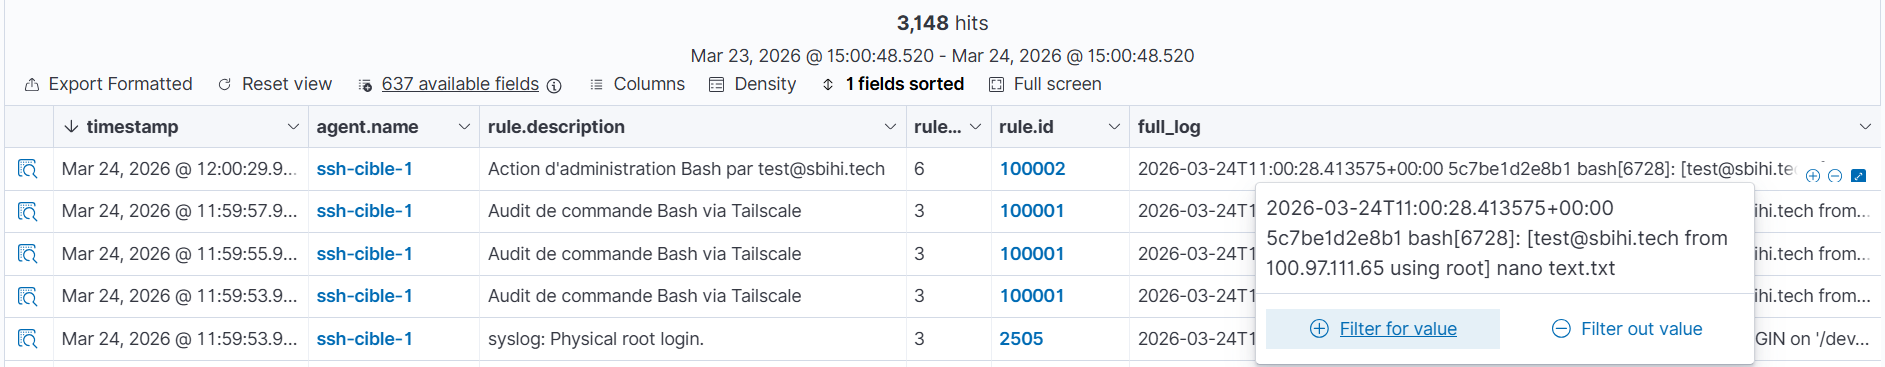
\includegraphics[width=0.97\textwidth]{images/wazuh_log_from ssh showing what the user did in after login to the ssh cible .png}
	\caption{Preuve TC-06: evenements Wazuh issus des commandes SSH journalisees sur la machine cible.}
	\label{fig:tc06-wazuh-ssh-audit}
\end{figure}
Ce test valide la chaine de tracabilite de bout en bout: commande utilisateur -> journal cible -> ingestion agent -> visualisation SIEM Wazuh.

\section{Resultats de validation}
Les tests attendus doivent confirmer les proprietes suivantes:
\begin{itemize}
	\item aucune elevation de privilege sans authentification forte;
	\item aucune activation de droit sans approbation explicite;
	\item aucune persistance d'acces au-dela de la fenetre autorisee;
	\item auditabilite de l'ensemble du cycle demande-approbation-expiration, incluant les commandes shell sur machine cible.
\end{itemize}

La section sera finalisee avec les resultats observes, les captures associees et les eventuelles non-conformites detectees durant les essais.

Les preuves inserees confirment la logique attendue par le modele Zero Trust: refus par defaut, autorisation explicite et temporalite stricte des privileges.

\section{Conclusion du chapitre}
La campagne de test proposee couvre les points critiques du cycle JIT: refus par defaut, approbation explicite, acces temporaire et revocation automatique. Ces verifications constituent la base de mesure des resultats presentes au chapitre suivant.

\chapterpage{Chapitre 7 : Resultats, metriques et discussion}

\chapter{Resultats, metriques et discussion}

\section{Introduction du chapitre}
Ce chapitre presente la lecture des resultats obtenus apres mise en oeuvre de la solution. Il compare la situation avant/apres, interprete les gains et discute la portee des effets observes sur la securite et la gouvernance des acces.

\section{Indicateurs avant/apres}
Les indicateurs de performance securite retenus sont presentes ci-dessous.

\begin{center}
\begin{tabular}{|p{4.2cm}|p{3.2cm}|p{3.2cm}|p{3.2cm}|}
\hline
\textbf{Metrique} & \textbf{Avant} & \textbf{Apres} & \textbf{Gain estime} \\
\hline
Acces privilegies permanents sur cibles critiques & Non maitrise & Controle JIT & Elimination des acces permanents non justifies \\
\hline
Duree moyenne d'acces privilegie & Illimitee & TTL borne (1h a 4h) & Forte reduction de la fenetre d'exposition \\
\hline
Sessions auditables & Partielle & Tracabilite de bout en bout & Couverture audit fortement amelioree \\
\hline
MFA sur parcours sensible & Non systematique & Generalise via IAM & Hausse majeure du niveau d'assurance \\
\hline
Reexecution post-expiration & Possible dans certains cas & Refusee par conception & Reduction du risque de privilege persistant \\
\hline
\end{tabular}
\end{center}

\section{Analyse des gains}
Les gains observes se situent sur trois axes:
\begin{itemize}
	\item \textbf{Securite}: reduction de la confiance implicite et application stricte du moindre privilege.
	\item \textbf{Gouvernance}: formalisation d'un workflow de demande/approbation explicite et controlable.
	\item \textbf{Auditabilite}: disponibilite de preuves techniques (captures, journaux, statuts applicatifs) pour les besoins de conformite.
\end{itemize}

La valeur metier est particulierement visible sur les interventions de remediation vulnerabilite, car chaque action privilegiee devient justifiee et rattachee a un contexte.

\section{Discussion}
Le prototype valide la faisabilite d'une architecture Zero Trust pragmatique avec des composants open source et des integrations legeres en Python.

Les principaux retours d'experience sont:
\begin{itemize}
	\item l'integration IAM + ACL + workflow applicatif est suffisante pour obtenir un resultat mesurable rapidement;
	\item la qualite de la preuve (captures, logs, commandes) est aussi importante que la logique technique;
	\item la maturite operationnelle dependra ensuite de l'industrialisation (CI/CD, supervision avancee, haute disponibilite).
\end{itemize}

\section{Conclusion du chapitre}
Les metriques et l'analyse confirment une amelioration tangible de la posture de securite sur les acces privilegies. Les resultats obtenus justifient la poursuite vers une phase d'industrialisation et d'extension du perimetre.

\chapterpage{Chapitre 8 : Limites et travaux futurs}
\chapter{Limites et travaux futurs}

\section{Introduction du chapitre}
Ce chapitre met en perspective les acquis du projet en identifiant les limites de l'état actuel et les évolutions prioritaires. Il permet de distinguer ce qui est valide dans le prototype de ce qui reste à consolider pour un usage de production.

\section{Limites identifiees}
Malgré les résultats obtenus, certaines limites doivent être explicitées :
\begin{itemize}
	\item déploiement orienté laboratoire, sans architecture haute disponibilité complète ;
	\item couverture de tests encore centrée sur les parcours critiques, non exhaustive sur tous les cas limites ;
	\item dépendance à des configurations manuelles pour certaines intégrations d'outils ;
	\item niveau de durcissement variable selon les environnements cibles.
\end{itemize}

\section{Pistes d'amelioration}
Les évolutions prioritaires à court terme sont :
\begin{itemize}
	\item automatiser davantage les tests de non-régression du workflow JIT ;
	\item enrichir les tableaux de bord de conformité (indicateurs périodiques, alertes) ;
	\item formaliser les procédures d'exploitation (runbooks incidents et révocation d'urgence) ;
	\item compléter la base de preuves pour les audits internes.
\end{itemize}

\section{Perspectives long terme}
A plus long terme, la solution peut évoluer vers :
\begin{itemize}
	\item une extension du périmètre à davantage d'actifs et d'équipes ;
	\item l'industrialisation complète (pipeline de déploiement, tests automatisés, gestion de secrets) ;
	\item une corrélation plus avancée entre vulnérabilités, exposition effective et identités actives ;
	\item un alignement renforcé avec les exigences GRC et les contrôles de conformité.
\end{itemize}

\section{Conclusion du chapitre}
Les limites constatées restent maîtrisables et principalement liées au niveau d'industrialisation. Les perspectives définies offrent une trajectoire claire pour faire évoluer le prototype vers une solution robuste et généralisable.

\chapterpage{Conclusion generale}
\chapter{Conclusion generale}

\section{Introduction du chapitre}
Ce dernier chapitre clot le rapport en synthetisant les apports principaux du projet et leur impact sur la securisation des acces privilegies dans une logique Zero Trust.

Ce projet a permis de concevoir et de valider une architecture Zero Trust adaptee a un besoin concret de maitrise des acces privilegies.

La contribution principale est la mise en place d'un parcours complet, depuis l'authentification forte jusqu'a la revocation automatique des droits, en passant par l'approbation humaine et la tracabilite.

Les objectifs initiaux ont ete couverts:
\begin{itemize}
	\item centraliser la verification d'identite via IAM;
	\item controler l'acces a la ressource via ACL et workflow d'approbation;
	\item rendre l'elevation de privilege temporaire, justifiee et auditable.
\end{itemize}

Au-dela de la realisation technique, le projet montre qu'une demarche Zero Trust est d'abord une logique d'ingenierie et de gouvernance: chaque acces doit etre explicite, limite dans le temps, et verifiable a posteriori.

\section{Retour sur la problematique}
La problematique initiale consistait a supprimer les acces permanents tout en conservant l'operationnel. Le prototype apporte une reponse pragmatique grace au JIT, a la journalisation et a l'approbation explicite.

\section{Contributions}
Les contributions principales sont la reduction de la surface d'attaque, l'amelioration de la tracabilite et la structuration d'un workflow exploitable pour la conformite.

\section{Ouverture}
Les evolutions futures peuvent aller vers un PAM plus complet, davantage d'automatisation et une meilleure integration avec les outils de ticketing et de politique centralisee.

\section{Conclusion du chapitre}
Le projet atteint son objectif central: transformer l'acces privilegie permanent en acces conditionnel, temporaire et auditable. Cette base constitue un socle solide pour une generalisation progressive a d'autres environnements et usages.

\chapter*{Bibliographie}

\bibitem{nist800207}
NIST. \emph{Zero Trust Architecture (SP 800-207)}.

\bibitem{authentik}
Authentik. \emph{Documentation officielle Authentik}.

\bibitem{tailscale}
Tailscale. \emph{Documentation officielle ACL et access control}.

\bibitem{wazuh}
Wazuh. \emph{Documentation officielle Wazuh}.

\bibitem{flask}
Pallets. \emph{Flask Documentation}.

\bibitem{postgresql}
PostgreSQL Global Development Group. \emph{PostgreSQL Documentation}.




\end{document}
